%==================================================================================================
%   LUKES THESIS TEMPLATE 1.2
%   -------------------------
%   This template is based upon the offcial IMM PhD Thesis template, it is enhanced with a number
%   of new features and a number of errors have fixed. This template is intended to be complied to
%   PDF using PDFLATEX and is tested using the MiKTeX 2.9 LaTeX distribution.
%   It is based on the official DTU-IMM Thesis template by Finn Kuno Christensen in 2009.
%   Small bugfixes by Kasper Laursen in 2012 and 2013.
%   -------------------------
%   Last Updated: 2012-09-19
%   Contact: lthhe@imm.dtu.dk
%==================================================================================================
%
%==================================================================================================
% DOCUMENT SETUP
%==================================================================================================
\documentclass[10pt,twoside,table]{book}                  %Official DTU-IMM Thesis document setup
%
%Set to 'print' for printed version, use 'net' for online version
\def\thesisversion{print}
%
%==================================================================================================
% PACKAGES
%==================================================================================================
\usepackage{LukeThesis}                            %Import Thesis base style
\usepackage{xcolor}
\usepackage{graphicx}
%\usepackage[utf8]{inputenc}
%\usepackage[T1]{fontenc}
%\usepackage{url}
\usepackage{xstring}
\usepackage{hyperref}
\usepackage{pdfpages}
\usepackage{placeins}
\usepackage[font=small,labelfont=bf]{caption}
\usepackage{subfig}

%\usepackage{subcaption}
\usepackage{enumerate}
\usepackage{amsmath}
\usepackage{listings} %for showing program code
\usepackage{bm}
\usepackage{wrapfig}
\usepackage{lipsum}
\usepackage{float}
\usepackage{titlesec}	
\usepackage{amsfonts}
\usepackage{amssymb}
\usepackage[square,authoryear]{natbib}
\usepackage{epstopdf}
\usepackage{tabularx}
\usepackage{siunitx}
\usepackage{mathtools}
\usepackage{tcolorbox}
\usepackage{lscape}
\usepackage{multirow}
\usepackage{setspace}
\usepackage{glslListings} 

\tcbuselibrary{breakable}

\newtcolorbox{mybox}{colback=red!3!white,colframe=red!75!black,breakable,arc=0pt,outer arc=0pt}

\bibpunct{[}{]}{,}{a}{,}{,}
\raggedbottom 
%\setlength{\parskip}{0pt}

%input{PhDMacros}                                   %Thesis specific macros
%
%==================================================================================================
% THESIS PROPERTIES (Modifiy these fields with your details)
%==================================================================================================
\def\thesisauthor{Alessandro Dal Corso}                     %Author
\def\thesistitle{Real-Time Rendering of Translucent Materials with Directional Subsurface Scattering}               %Title
\def\thesishandin{03-July}                       %Submission date (Day-Month}
\def\thesisdegree{M.Sc.}                              %Degree ('B.Eng', 'B.Sc.', 'M.Sc.' or 'PhD')
\def\thesisyear{2014}                               %Submission year
\def\thesisnumber{????}                             %DTU-IMM Serial number (do not include year)
\def\thesisISSN{0000-0000}                          %ISSN number
\def\thesiskeywords{subsurface,scattering,realtime,directional,dipole}  %PDF keywords
\derivethesisprops                                  %Derive dependent properties
%
%==================================================================================================
% SECTION NUMBERING SETUP
%==================================================================================================
\setcounter{tocdepth}{2}                            %2 adds sections up to subsections
\setcounter{secnumdepth}{3}                         %Subsubsections get a number when this is 3

\begin{document}
%------------------------
%Pre-frontmatter material
%------------------------
%\prefrontmatter
%-------------------- 
%Frontmatter material
%--------------------
%\frontmatter
%\pagenumbering{roman}                               %Set frontmatter numbering style
%\chapter{Summary (English)}

The goal of the thesis is to ...                                   %English summary of Thesis
%\markboth{}{}                                       %Set headings (left)(right)
%\chapter{Summary (Danish)}
\begin{otherlanguage}{danish}

Målet for denne afhandling er at ...

\end{otherlanguage}                                   %Danish summary of Thesis
%\markboth{}{}                                       %Set headings (left)(right)
%\chapter{Preface}

\vspace{1cm}
This thesis was prepared at the DTU Compute department at the Technical University of Denmark in fulfillment of the requirements for acquiring an M.Sc. in Digital Media Engineering. 

The thesis deals with the efficient rendering of translucent materials, using an innovative model proposed by the author's M.Sc. thesis supervisor, Jeppe Revall Frisvad. Translucent materials consist of a particular class of materials like fruit, marble, skin, and other materials where subsurface scattering effects cannot be neglected. 

The interest for real time rendering in the author arose during the course of his M.Sc. in Digital Media Engineering, where he focused on the study line in Computer Games. For this study line, he had to take several courses in real time computer graphics, and from this courses he got his interest in advanced shading techniques. In the spring 2014, professor Jeppe Revall Frisvad of DTU Compute proposed a research-oriented M.Sc. thesis, that had the final goal of creating a method for implementing the directional dipole in real time. The author deemed the topic to be a great opportunity to research in real time rendering techniques, and so he registered his application for this master thesis, \emph{\thesistitle}.

The thesis consists of a software implementation in C++, Qt and OpenGL, and this report. The initial Qt framework used was taken from DTU course 02564, \emph{Real Time Graphics}, and then expanded in order to fit the needs of the thesis. All the code reported in this document was written by the author an does not come from the original framework. All the screenshots in this document were generated using the developed software. Other images in the report, unless the original source is reported in the caption, were generated by the author.

%==================================================================================================
% SIGNATURE AREA
%==================================================================================================
\begin{table}[ht]
\begin{tabularx}{\textwidth}{X}
\vspace{1.5cm}
Lyngby, \thesishandin-\thesisyear \\
\hfill \thesisauthor \\
\hfill 
\includegraphics[scale=0.4]{images/sig.png} \\
\end{tabularx}
\end{table}                                     %Preface
%\markboth{}{}                                       %Set headings (left)(right)
%\chapter{Acknowledgements}

I would like to thank my....

                            %Acknowledgements
%\markboth{}{}                                       %Set headings (left)(right)
%------------------
% Table of contents
%------------------
%\newpage\mbox{}\newpage
\chaptermark{Contents}
\pdfbookmark{\contentsname}{toc}
\renewcommand{\sectionmark}[1]{\markright{#1}}
\sectionmark{Contents}
\addtolength{\parskip}{-\baselineskip}
\tableofcontents
\addtolength{\parskip}{\baselineskip}
\renewcommand{\sectionmark}[1]{\markright{\thesection\ #1}}
%-------------
% Main content
%------------- 
\mainmatter
\newcommand{\vomega}{\vec{\omega}}
\newcommand{\x}{\mathbf{x}}
\newcommand{\cs}{C_{\phi}(\eta)}
\newcommand{\csinv}{C_{\phi}(1/\eta)}
\newcommand{\ce}{C_{\mathbf{E}}(\eta)}
\newcommand{\projt}{\rotatebox[origin=c]{180}{T}}
\chapter{Introduction}
\label{chap:intro}
\emph{Subsurface scattering} (SS) is a physical phenomenon that naturally occurs in a wide range of natural materials. Some materials that exhibit a strong subsurface scattering effect in everyday life are milk, human skin and marble. Subsurface scattering occurs when light is partially absorbed by an medium, bounces repeatedly inside ("scatters") and finally exits the surface on another point of the material (as in Figure \ref{fig:ssdiagram}). The phenomenon that results is generally known as \emph{translucency}. We can see some examples of translucent objects in Figure \ref{fig:ex1}.

\section{Background}
Since the beginning of computer graphics, various attempts have been performed in order to model subsurface scattering. Some of these models involve Monte Carlo simulations of the light entering the medium \citep{Pharr:2000:MCE:344779.344824}, or other numerical techniques \cite{Fattal:2009:PMI:1477926.1477933,Kaplanyan:2010:CLP:1730804.1730821}. Other focus on approximating the diffusion of light within the material using an analytical approach, like \citep{Jensen:2001:PMS:383259.383319}.
 
\clearpage
\begin{figure}[!ht]
\centering
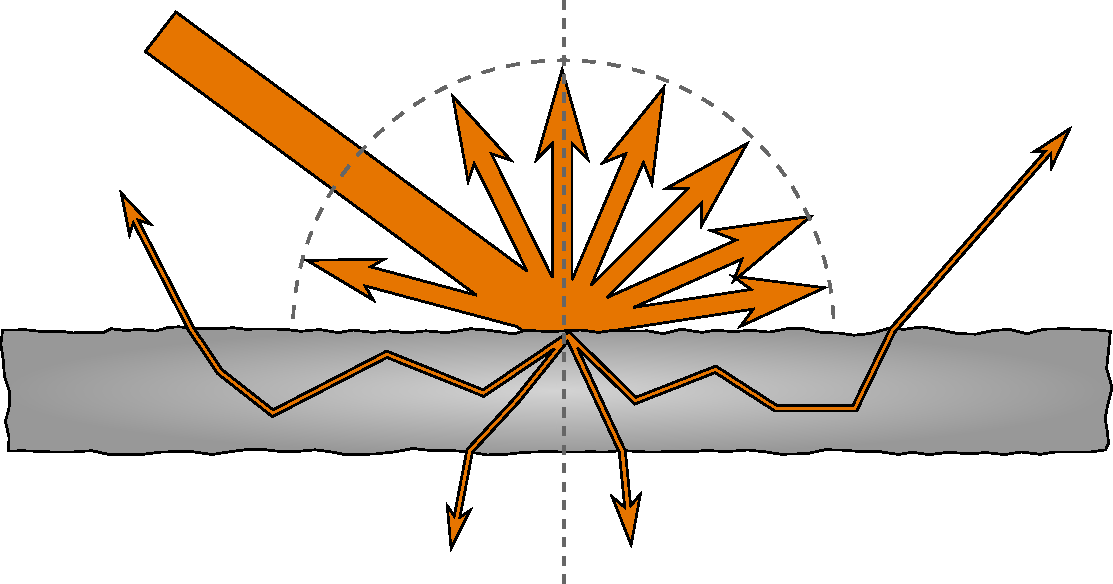
\includegraphics[width=0.8\textwidth]{images/diagram.pdf}
\caption{Diagram of subsurface scattering. Most of the incoming light gets reflected, but some of it enters the material and leaves it at a different point.}
\label{fig:ssdiagram}
\end{figure}

The first model that proposed an analytical approach was the one by \cite{Jensen:2001:PMS:383259.383319}, as an approximation of the radiative transfer equation. This approximation, called the \emph{diffusion approximation} \citep{books/daglib/0093591} has been exploited by different authors, in order to account for multi-layered materials \citep{Donner:2005:LDM:1186822.1073308}, heterogeneous materials \citep{journals/cgf/WangWHSYG10} and thin surfaces\citep{journals/cgf/WangWHSYG10}. A recent analytical model, proposed by \cite{IMM2013-06646}, extends the approximation in order to account for the directionality of the incoming light. All these analytical methods are based on BSSRDF models. A BSSRDF function is a functions that describes how light is transmitted between two points in a material, and is a generally dependent on the incoming light direction, the distance between the two points and the outgoing light direction.

In recent years, with the advent of programmable graphics cards (GPU), it has become possible to exploit these algorithms and bring them to interactive frame rates, and in some cases even to real time rendering. \cite{Jensen:2002:RHR:566654.566619} were the first to propose an efficient implementation for rendering subsurface scattering using an octree. More recently, several methods have been proposed, including image-based splats \citep{4736459}, sum-of-Gaussians filtering \citep{d'Eon:2007:ERH:2383847.2383869}, and grid-propagation based methods \citep{Borlum:2011:SSL:2018323.2018325}. We will introduce in detail some of these methods in Chapter \ref{chap:previous}, were we will review the existing literature in more detail.

\begin{figure}
\centering
\subfloat{
  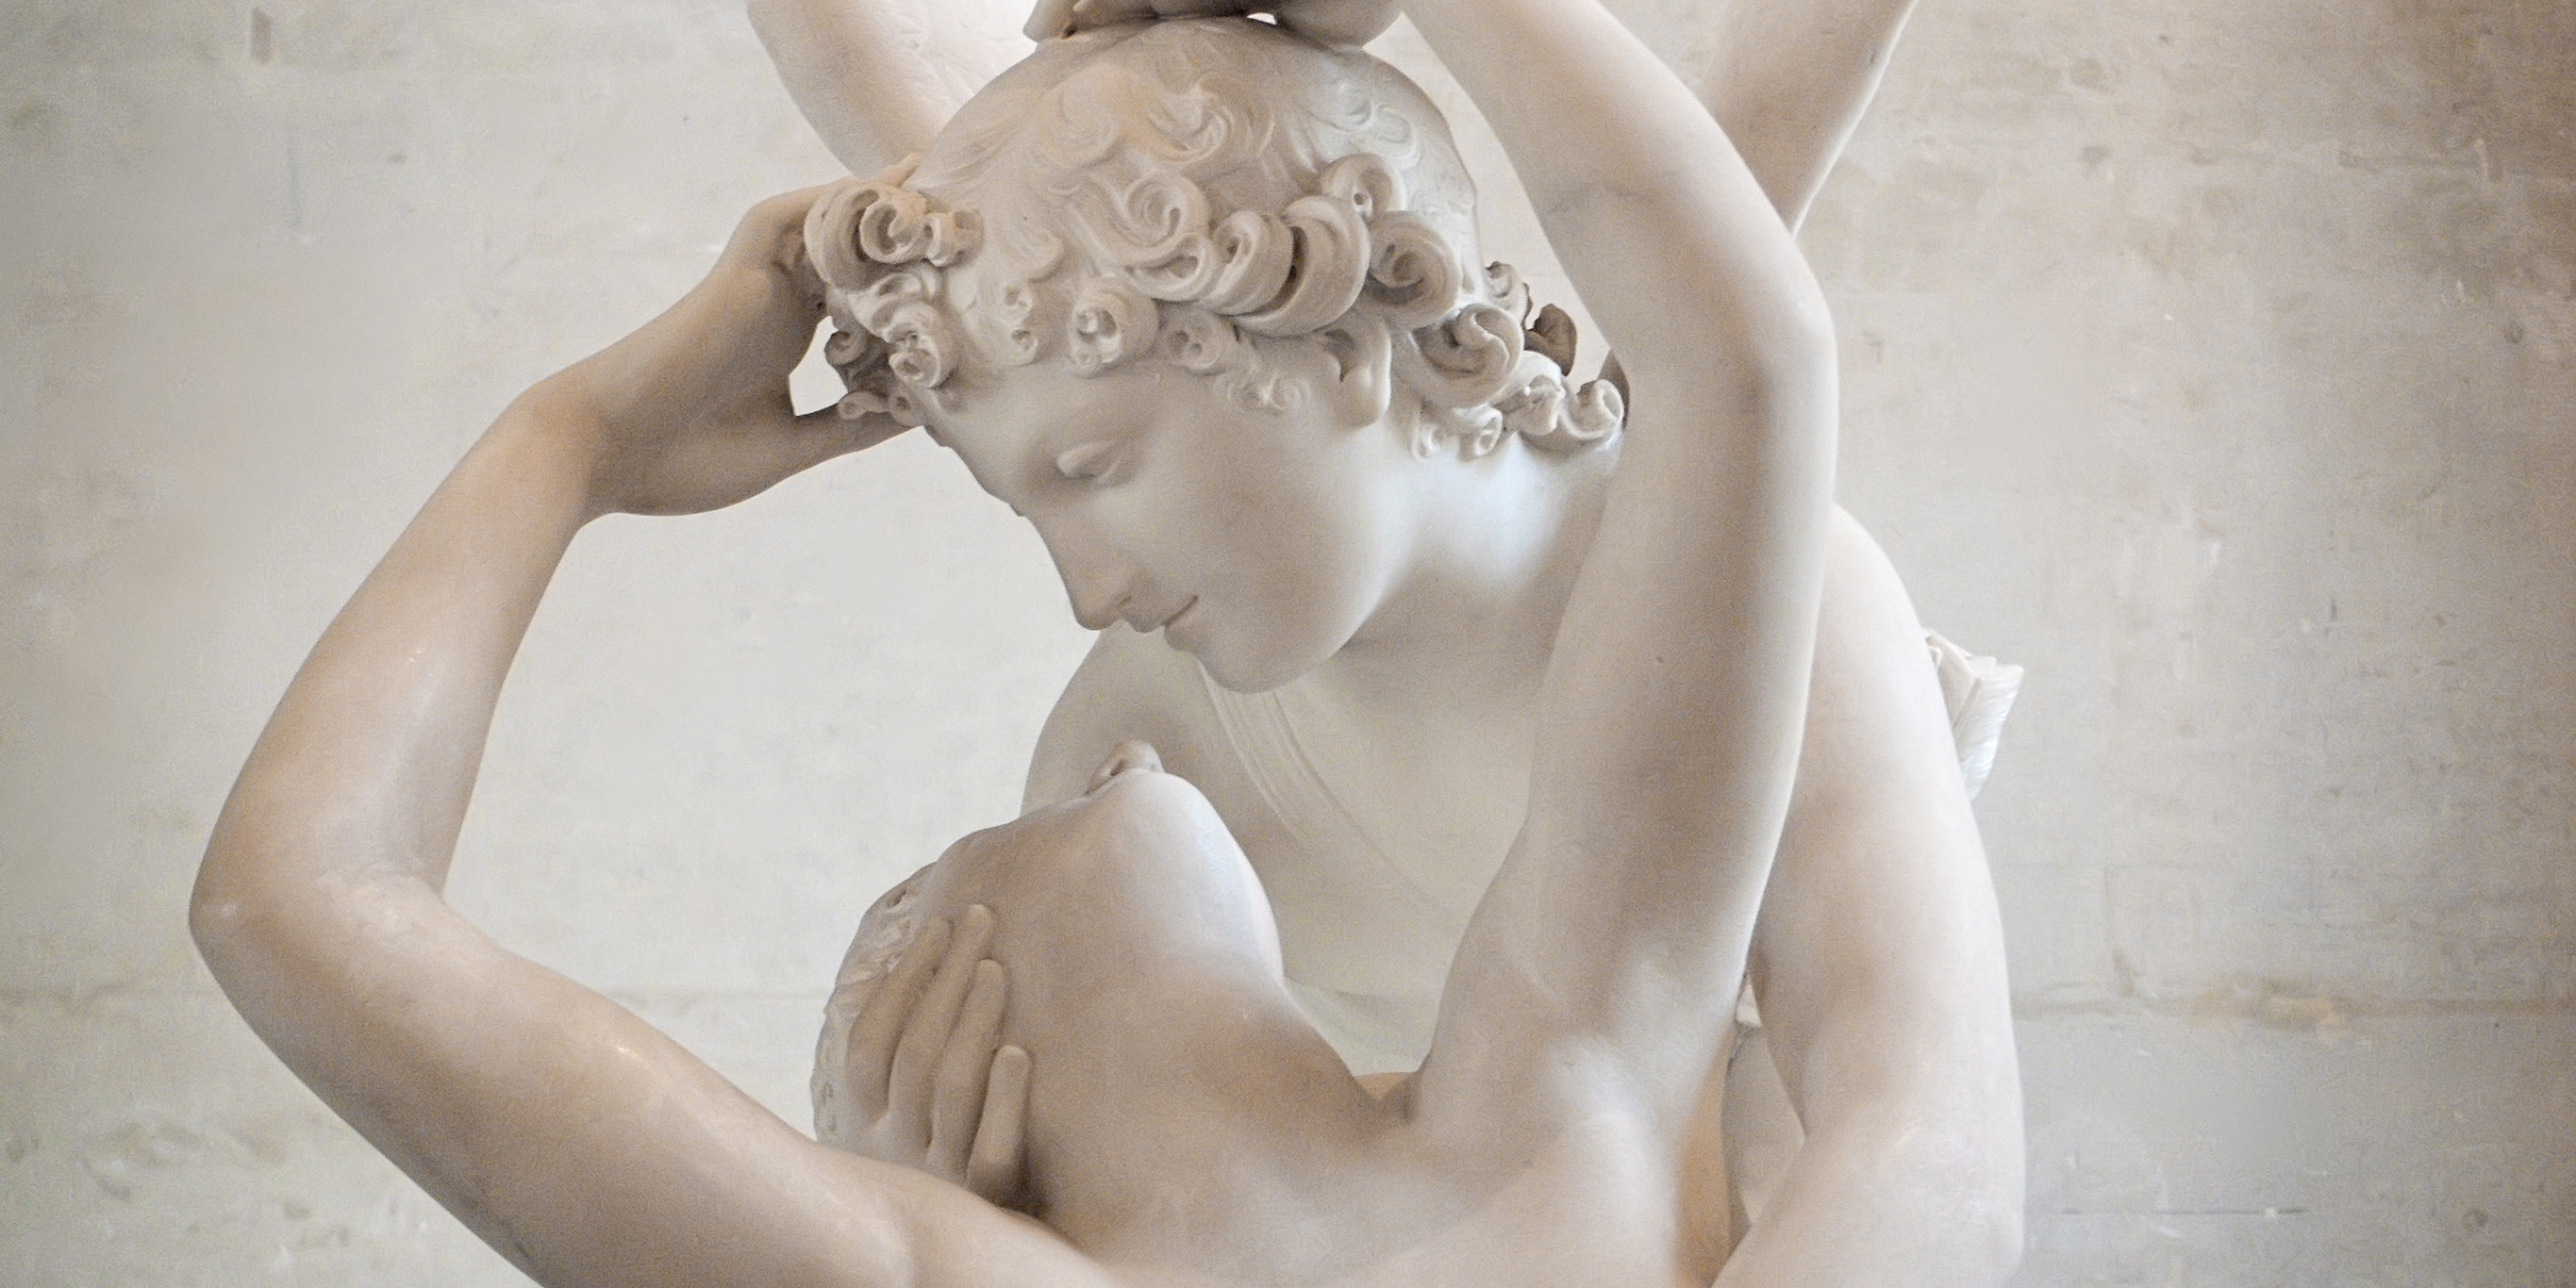
\includegraphics[width= 0.9 \linewidth]{images/marble.jpg}
  \label{fig:ss1}
}
\\
\subfloat{
  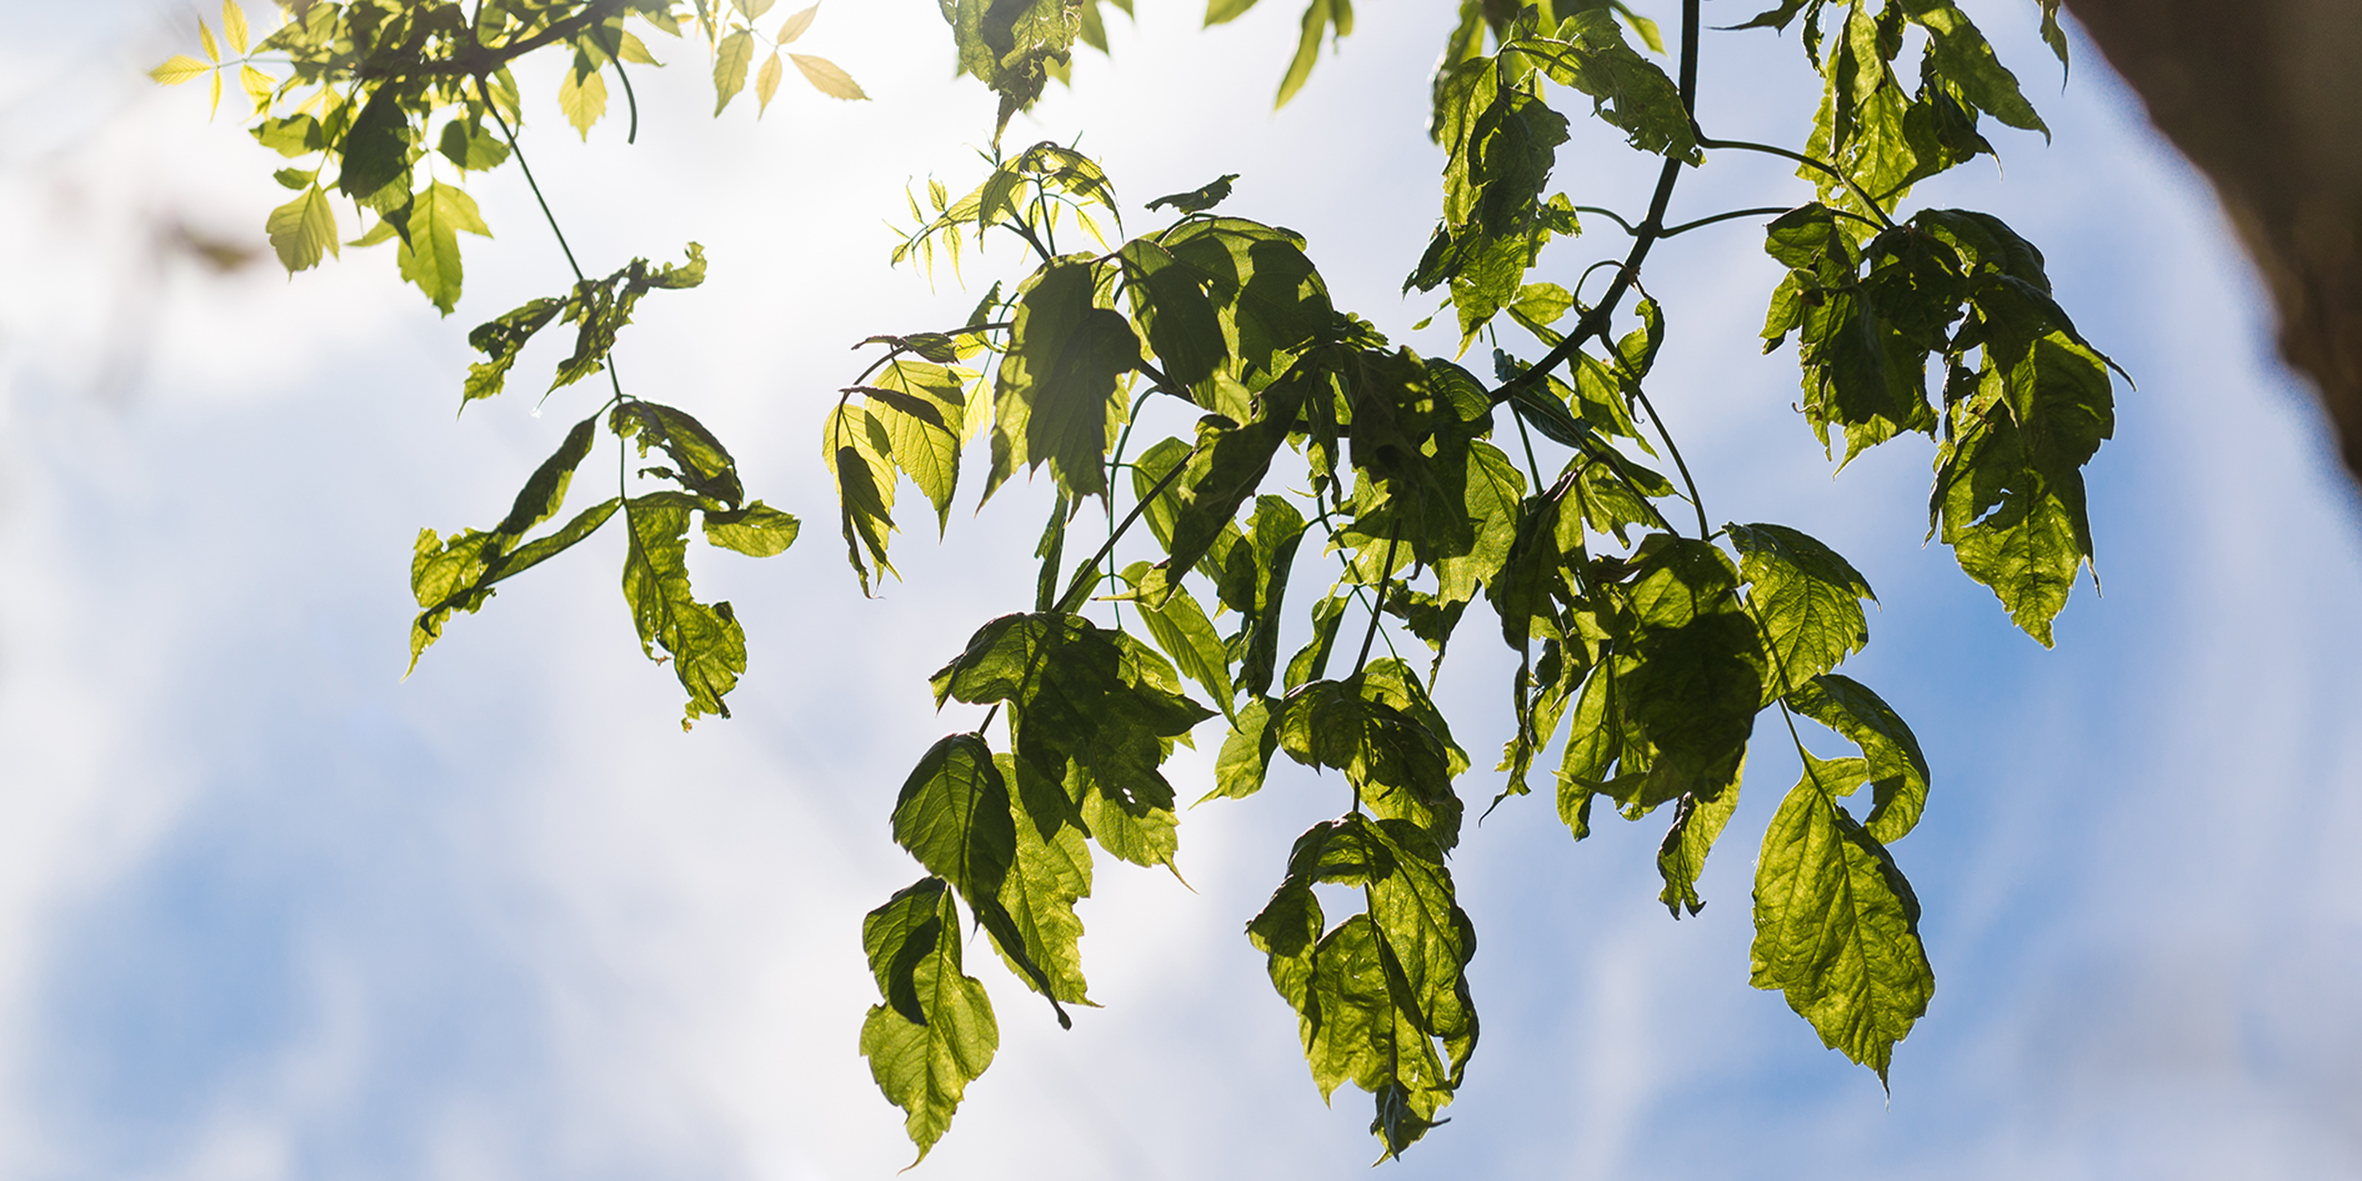
\includegraphics[width= 0.9 \linewidth]{images/leaves.jpg}
  \label{fig:ss2}
} 
\\
\subfloat{
  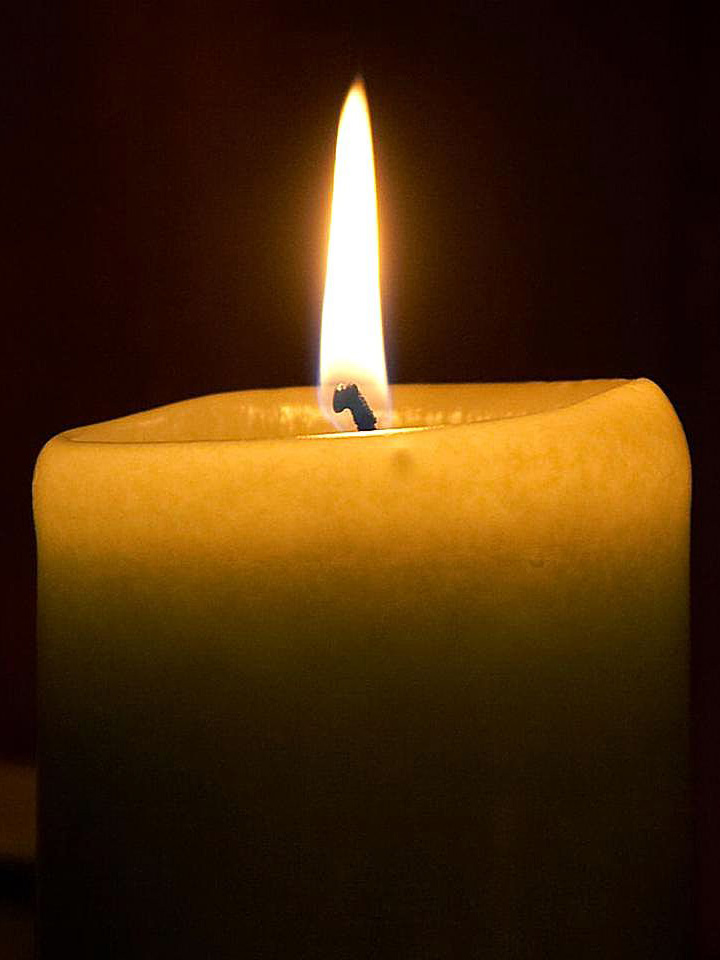
\includegraphics[width=0.9 \linewidth]{images/candle.jpg}
  \label{fig:ss3}
} 
\caption{Some examples of translucent materials: marble, leaves and wax. The marble image and the candle are under the \href{http://creativecommons.org/licenses/by-sa/2.0/deed.en}{cc-by-sa} license, and are courtesy of Wikimedia Commons. The two images were cropped to fit the document. The leaves image was taken by Alberto Bedin and is used with permission.}
\label{fig:ex1}
\end{figure}

\section{Problem statement}

The goal of this thesis is to implement a real-time rendering technique in order to render directional subsurface scattering using the analytical model proposed by \cite{IMM2013-06646}. The technique should ideally obtain the same results as a offline rendered solution of the original model, but reducing the rendering times to a few milliseconds. To do this, we employ the aid of the GPU programmable pipeline \citep{Fernando:2004:GGP:983868}. 

We found that there is a current gap in the knowledge on current real-time subsurface scattering techniques regarding the approach to directional models. In fact, most of the methods rely on the assumption that the BSSRDF function depends only on the distance between the entering and exiting point \cite{Jensen:2001:PMS:383259.383319}. This allows, for example, to pre-compute the BSSRDF function and use it in the computations, greatly increasing the performance \citep{4736459}. However, in the model proposed by \cite{IMM2013-06646}, this is not possible, as the direction of the incoming light must be taken into account. In fact, the model has too many degrees of freedom to make a pre-computation feasible. 

The model proposed by \cite{IMM2013-06646} offers a more realistic evaluation of subsurface scattering effects. A real-time working implementation would improve the quality of scattering materials in real-time graphics applications, such as real-time architectural visualization and computer games. In the latter field, in recent years there has been a renewed interest in real-time SS techniques, especially to model faithfully the appearance of skin on human faces. 

\section{Requirement analysis}

In this section, we will introduce some constraints and assumptions to limit the scope of our work. Some of these assumptions and constraints are well known to the graphics community, and they are generally introduced to allow better performance, quality and flexibility. Being a real-time rendering method implies that performance plays a big part in the decisions we have made in the process, but since the method uses a physically based approximation the final quality of the result is also important. In the process the aspect of flexibility has been taken into account, i.e. the capacity of the method to set the tradeoff between quality and performance. We will now list the assumptions we made in all the three described domains, quality, performance and flexibility. 

\subsection{Quality constraints}
 \label{sec:quality}
\begin{enumerate}
\setlength{\itemsep}{-1pt}
	\item Be visually close as much as possible to a offline rendered solution.
	\item Be consistent with the directional dipole model for a wide range of material properties. In particular, the method should perform well in the domain of quality where the directional dipole model excels (highly scattering materials).
	\item Be potentially able to render an object under an arbitrary number of different types of lights (point, directional, environment, etc.).
\end{enumerate}

\subsection{Flexibility requirements}	
\begin{enumerate}
\setlength{\itemsep}{-1pt}
	\item Work with the less amount as possible of provided model data, i.e. only the position data and eventually the normals should be provided in order for the method to run. In particular, no unwrap of the mesh (UV mapping) should be necessary. 
	\item Being able to be integrated in a game engine environment, using data from other computations (e.g. other lighting computations) and being adaptable to different lighting paths (forward and deferred shading).
  \item The quality versus performance tradeoff should be set by a potential artist or developer, with the fewest number of parameters as possible.
\end{enumerate}

\subsection{Performance requirements}
\begin{enumerate}
\setlength{\itemsep}{-1pt}
	\item Being real-time on a high-end modern GPU, i.e. one frame should take less that 100 ms (10 FPS) to render. The ideal result would be to reach a rendering time of less than 16 ms (60 FPS).
	\item Being as less dependent as possible from the geometrical complexity of the model.
	\item Being as less dependent as possible from the screen resolution.
	\item If the desired quality is not reachable within one frame, converge towards a result in a reasonable amount of time. Techniques should be used to approximate the required quality for the intermediate result. 
	\item Maintain a reasonable performance under changing light conditions, deformations and change of parameters, with little or none performance penalties.
	\item Employ the advantages of the directional dipole model to improve performance.
	\item Support up to a certain number of directional and point lights (up to 3 to 5 pixel lights, as in commercial engines\citep{unitymanual}).
	\item Require little or no pre-processing in order to be able to perform. If there is any pre-processing involved, it should be performed only at the beginning of the life cycle of the program. 
\end{enumerate}

%\section{Method overview}
%
%Our method consists of introducing the assumption that only the points within a certain radius from the point are contributing to the exiting light. Then, we take a certain number $N$ of these surface samples and compute their contribution to calculate the exiting light. The samples are distributed with an exponential distribution, in order to account more for the samples closest to the exiting point. The reader can get more details on the method in Chapter \ref{chap:method}. 

\section{Thesis Outline}
In this Chapter, we have given an introduction to the problem and stated the assumption that will guide us through the choices that we will make through our thesis. In Chapter \ref{chap:previous}, Related Work, we will describe in more detail some of the different approaches to subsurface scattering in literature. In Chapter \ref{chap:theory}, we will give a theoretical introduction to subsurface scattering and light transport theory, with a special focus on BSSRDF functions. In Chapter \ref{chap:method}, we will describe our method on approaching the problem on a theoretical basis. In Chapter \ref{chap:implementation} we will describe the actual implementation of the method, and the problems and limitations met during the process. In Chapter \ref{chap:results}, we will describe the tests we made and show the results, both in the domain of performance and quality, comparing them with the requirement analysis we made in the previous section. Then, we will describe some possible extensions to the method in Chapter \ref{chap:futurework}. We will wrap up everything in Chapter \ref{chap:conclusions}, where we will give our conclusions. 
\chapter{Related Work}
\label{chap:previous}
In rendering of subsurface scattering, most approaches rely on approximating correctly the \emph{Radiative Transfer Equation} (RTE). We identified two main approaches to the problem in literature:

\begin{description}
	\item[Analytical] One class of solutions consists of approximating the RTE or one of its approximations via an analytical model. These models can have different levels of complexity and computation times, and are often adaptable to a wide range of materials. However, often they rely on assumptions on the scattering parameters that limit their applicability.
	\item[Numerical] In this other class of solutions, a numerical approach is used instead of approximating the RTE with an analytical model. This methods include finite element methods and discrete ordinate methods, for which a numerical solution for the RTE is actually computed. While providing an exact solution, the computation times are longer. Other numerical approaches focus more on the appearance of the model and do not provide an exact solution for the RTE.
\end{description}

In this thesis, we focus on efficiently implementing a model that falls in the first category, the analytical models. In the following sections, we are going to describe approaches for each one of the mentioned categories, comparing them to our method.

\section{Analytical techniques}

In the analytical techniques, two different areas of research must be distinguished. The first area is the research on the actual models, while the second is research on how the actual models can be implemented efficiently. Each model is usually represented by a specific function called BSSRDF (\emph{Bidirectional Subsurface Scattering Reflectance Distribution Function}), that describes how light propagates between two points on the surface. Two integrations, one on the surface one from all the directions, must be performed in order to get the amount of light that actually exits from a point on the surface (see chapter \ref{chap:theory}). Implementation techniques focus on efficiently implementing this integration steps, often making assumptions for which points computations can be avoided. 

\subsection{Models}
Regarding the models, the first and most important is the dipole developed by \cite{Jensen:2001:PMS:383259.383319}. This models relies on an approximation of the RTE called the \emph{diffusion approximation}, which again relies on the assumption of highly scattering materials. In this case, a BSSRDF for a planar surface in a semi-infinite medium can be obtained. The BSSRDF needs only the distance between two points to be calculated, and with some precautions can be also used with arbitrary geometry. This model does not include any single scattering term: it needs to be evaluated separately. The model has been further extended in order to account for thin object regions and multi-layered materials \citep{Donner:2005:LDM:1186822.1073308}.

A significant improvement of the model was later given by \cite{deondeon}, that improved the model to better fit path traced simulations without nearly any additional computation cost. A more advanced model based on quantization was proposed by \cite{D'Eon:2011:QMR:1964921.1964951}, that introduced a new physical foundation in order to improve the accuracy of the original diffusion approximation. Finally, some higher order approximation exist \citep{PhysRevLett.94.153904, IMM2013-06646}, in order to account for the directionality of the incoming light and single scattering. This allows a more faithful representation of the model at the price of extended computation times. A comparison between the directional and the standard dipole can be seen in figure \ref{fig:bssrdfcomparison}.


\subsection{Implementations}

Most research on efficient implementations of a subsurface scattering analytical model has been made on the original model by \cite{Jensen:2001:PMS:383259.383319}. The first efficient implementation was proposed by \cite{Jensen:2002:RHR:566654.566619}, based on a two-pass hierarchical integration approach. Samples on the model are organized in an octree data structure, that then is used to render the object. In the first step, the radiance from the light is stored in the points. In the second pass, using the octree, the contribution from neighboring points is computed, clustering far points in order to speed up calculations. This approach can be adopted for the Jensen model, where the only parameter is the distance between the entering and exiting point. However, using the directional dipole, the samples cannot be clustered because of the directionality of the light: once we sum up the contribution from multiple lights, the contribution cannot be separated anymore. In fact, we would need a different clustering of the points for each light, that quickly becomes inefficient since whole octree would have to be stored on the GPU. 

\cite{Lensch:2002:IRT:826030.826632} approached the problem by subdividing the subsurface scattering contribution into two: a direct illumination part and a global illumination part (i.e. the light shining through the object). The global illumination part is pre-computed as vertex-to-vertex throughput and then summed to the direct illumination term in real-time. Compared to our method, this method requires a pre-computation step that depends on the geometry of the model, and thus deformation effects are not possible. Moreover, a coefficient has to be stored for each pair of vertex, that means a quadratic increase for increasing model size. Our method, on the other hand, occupies a memory space depending linearly on the number of vertices.

Translucent shadow maps \citep{Dachsbacher:2003:TSM:882404.882433} use an approach similar to standard shadow maps: they render the scene from the light point of view, and then calculate the dipole contribution in one point only from a selected set of points, according to a specified sampling pattern. As in \cite{Lensch:2002:IRT:826030.826632}, the contribution is split into global and local to permit faster computations. In our approach we will reuse some of the ideas introduced by translucent shadow maps: we will render the scene from the light point of view and we will reuse the information stored in the map such as depth, vertices and normals. However, our approach to using the values from the map is different from the original paper, as we will explain in chapter \ref{chap:method}. \cite{Mertens:2003:IRT:882404.882423} propose a fast technique based on radiosity hierarchical integration techniques, that unlike the previous implementation can handle deformable geometry.

Another important category of methods is screen space methods. \cite{1238246} propose an image space GPU technique that pre-computes a set of sample points for the area integration and then performs the integral over multiple GPU passes. \cite{d'Eon:2007:ERH:2383847.2383869,deonss} propose a method in image-space, interpreting subsurface scattering as a sum of images to which a gaussian filter has been applied. The gaussians are then summed with weights that make them fit the diffusion approximation. \cite{Jimenez:2009:SPR:1609967.1609970} improves further the technique, giving more precise results in case of skin. All these techniques assume that the diffusion profile can be pre-computed and then fitted with a sum of Gaussians: as we have already mentioned, this is not possible for the directional dipole, where the diffusion profile can change a lot depending on the angle of incidence of the incoming ray of light. Moreover, even if we were able to compute the coefficients for each possible combination of parameters, it would not be possible to apply a gaussian filter with a different set of coefficients per point.

\cite{4736459} present a fast screen space technique that render the object as a series of splats, using GPU blending to sum over the various contributions. The diffusion profile in this case is pre-computed and stored as a texture. As in the previous techniques, the directionality of the incoming light does not allow the pre-computation of a diffusion profile. Moreover, the directional dipole is not symmetrical, so the splats would have to use a bigger radius in order to account for all the contribution, increasing computation costs.

\section{Numerical techniques}

Numerical techniques for subsurface scattering are often not specific, but come for free or as an extension of a global illumination numerical approximation, since the governing equations are essentially the same. Given their generality, they are usually slower than their analytical counterpart, and often rely on heavy pre-computation steps in order to achieve interactive framerates. The volumetric version of Jensen's Photon Mapping\citep{Jensen:1998:ESL:280814.280925} was originally developed to render participating media in general, but it has been adapted for subsurface scattering\citep{Dorsey:1999:MRW:311535.311560}. Classical approaches as a full Monte-Carlo simulation implementation of the light-material interaction, and finite-difference methods exist in literature\citep{raey}. 

Some less general methods have been introduced in order to devise more efficient approximations when it comes to the specific problem of subsurface scattering. \cite{raey} uses the diffusion approximation with the finite difference method on the object discretized on a 3D grid. \cite{Fattal:2009:PMI:1477926.1477933} uses as well a 3D grid, that is swept with a structure called light propagation map, that stores the intermediate results until the simulation is complete. All the numerical methods described so far are not real-time, and they are generally not feasible for a GPU environment. 

\cite{journals/cgf/WangWHSYG10}, instead of performing the simulation on a discretized 3D grid, makes the propagation directly in the mesh, converting it into a connected grid of tetrahedrons called \emph{QuadGraph}. This grid can be optimized to be GPU cache friendly, and provide a real-time rendering of deformable heterogeneous objects. The problem in this method is that the QuadGraph is slow to compute (20 minutes for very complex meshes) and has heavy memory requirements for the GPU. Compared to our method, this one requires an heavy pre-computation step, and allows only not-deformable objects. However, as most of propagation techniques, it can handle heterogeneous materials, while our method can not.

Precomputed radiance transfer methods are another class of general global illumination methods, that generally pre-compute part of the lighting and store it in tables\citep{Donner:2009:EBM:1531326.1531336}, allowing to retrieve it efficiently with an additional memory cost. The problem with this method compared to ours is that it requires a memory space that increases exponentially if we want to handle deformable materials and dynamic lighting. Moreover, it requires an heavy pre-computation in order to calculate the lighting coefficients. Our method, being analytical, does not required either a lot of memory or an heavy pre-computation step. 

A recent method called SSLPV (\emph{Subsurface Scattering Light Propagation Volumes}) \citep{Borlum:2011:SSL:2018323.2018325} extends a technique originally developed by \cite{Kaplanyan:2010:CLP:1730804.1730821} to propagate light efficiently in a scene using a set of discretized directions on a 3D grid. The method allows real-time execution times and deformable meshes with no added pre-computation step, with the drawback of not being physically accurate. Moreover, the required memory space on the GPU is larger than the one required than our method, since a voxelization of a mesh must be stored. 

Finally, for real-time critical applications (such as games), translucency is often estimated as a function of the thickness of the material, that is used to modify a lambertian term \citep{Tomaszewska2012,greenrtss}. A method by \cite{Kosaka:2012:RAR:2407156.2407206} uses an approach similar to the one we will describe in order to compute the thickness of the material using a different camera direction. While not physically accurate, this techniques allows to have a fast translucency effect that can be easily added to existing deferred pipelines. Compared to our method, this method requires no storage space and light computation. However, the risk is that the translucency effects are not represented faithfully, and some artifacts may appear, as pointed out in \cite{greenrtss}, and multi-sampling should be used in order to avoid artifacts. 

As we can see, in the reviewed literature so far there is not a proper way to account for direction in subsurface scattering in real-time, or at least one that satisfies the requirements we have made in chapter \ref{chap:intro}. We will introduce in detail our method to handle directional subsurface scattering in real-time in chapter \ref{chap:method}. In the next chapter, we are going to give a theoretical introduction to a mathematical description of light transport, as well as giving the proper formulas and definition of the standard dipole model by \cite{Jensen:2001:PMS:383259.383319} and the directional dipole model presented by \cite{IMM2013-06646}. 

\chapter{Theory}
\label{chap:theory}

In this chapter, we give a theoretical introduction to the topic dealt with in this thesis. The ultimate goal of this chapter is to introduce and describe analytical models for subsurface scattering. First, we will give a brief introduction to the nature of light, and how we physically describe it. Secondly, we will introduce the basic radiometric quantities that will be used throughout the chapter. Then, we will describe how this quantities are related and can be used to describe light-material interaction, using reflectance functions, of which BSSRDF functions are a special case. Finally, we will introduce subsurface scattering and the diffusion approximation, concluding with a description of two BSSRDF models, by \cite{Jensen:2001:PMS:383259.383319} and \cite{IMM2013-06646}.


\renewcommand{\arraystretch}{1.2}
\begin{table}[!ht]
\rowcolors{2}{white}{myblue}
\begin{tabular}{|l|l|}
\hline
Quantity                           & Description                                             \\ %\hline
$\mathbf{x}$                       & Point, not normalized vector                            \\ %\hline
$(x_x,x_y,x_z)$                    & Components of a vector                                  \\ %\hline
$\vec{\omega}$                     & Normalized vector, direction                            \\ %\hline
$Q$                                & Radiant Energy                                          \\ %\hline
$\Phi$                             & Radiant Flux                                            \\ %\hline
$E$                                & Irradiance                                              \\ %\hline
$I$                                & Intensity                                               \\ %\hline
$L$                                & Radiance                                                \\ %\hline
$\vec{n} \cdot \vec{m}$            & Dot product between two vectors                         \\ %\hline
$\vec{n} \times \vec{m}$           & Cross product between two vectors                       \\ %\hline
$A$                                & Area                                                    \\ %\hline
$i$ (subscript)                    & Denotes incoming direction or incidence point           \\ %\hline
$o$ (subscript)                    & Denotes outgoing direction or exitance point            \\ %\hline
M (capital letter)                 & Denotes matrix (see Appendix A)                         \\ %\hline
$f(...)$                           & BRDF function                                           \\ %\hline
$S(...)$                           & BSSRDF function                                         \\ %\hline
$\eta = \frac{n_1}{n_2}$           & Relative index of refraction                            \\ %\hline
$R(\eta,\vec{\omega})$             & Fresnel reflection term                                 \\ %\hline
$T(\eta,\vec{\omega})$             & Fresnel transmission term                               \\ %\hline
$\vec{\nabla} \cdot \vec{x}$       & Directional derivative of vector $\vec{x}$              \\ %\hline
$\sigma_a$                         & Absorption coefficient                                  \\ %\hline
$\sigma_s$                         & Scattering coefficient                                  \\ %\hline
$g$                                & Mean cosine coefficient                                 \\ %\hline
$\sigma_t = \sigma_s + \sigma_a$   & Extinction coefficient                                  \\ %\hline
$\sigma'_s = \sigma_s (1-g)$       & Reduced scattering coefficient                          \\ %\hline
$\sigma'_t = \sigma'_t + \sigma_a$ & Reduced extinction coefficient                          \\ %\hline
$\sigma_{tr}$                      & Transmission coefficient                                \\ %\hline
$\alpha'$                          & Reduced albedo                                          \\ %\hline
$\cs$                              & Approximation of the scalar fluence Fresnel integral    \\ %\hline
$\ce$                              & Approximation of the vector irradiance Fresnel integral \\ \hline
\end{tabular}
\caption{Table of the notation used in this thesis.}
\end{table}
\FloatBarrier

\section{Light and Radiometry}
Light is a form of electromagnetic radiation, that propagates through space as a sinusoidal wave. Usually by \emph{light} we refer to \emph{visible light}, the small part of the electromagnetic spectrum the human eye is sensible to (see Figure \ref{fig:spectrum}). This small window is between the \SI{380}{\nano\meter} of infrared and \SI{750}{\nano\meter} of ultraviolet light, but the precise boundaries may vary according to the environment and the observer. Instead explicitly noted, we will use the terms light and visible light interchangeably in this report.

The study of light is usually referred as \emph{optics}. In computer aided image synthesis, we are interested in representing faithfully how visible light propagates how it interacts with the objects and the materials in a scene. In addition, we are interested in lighting effects that are noticeable at human scales (\SI{1}{\milli\meter} - \SI{1}{\kilo\meter}), like subsurface scattering, absorption and emission phenomena. Optics studies more effects, like diffraction, interference and quantum effects, but we are not interested in representing them because for visible light they happen on a microscopic scale (\SI{1}{\nano\meter} - \SI{1}{\micro\meter}). 

\begin{figure}[!ht]
\centering
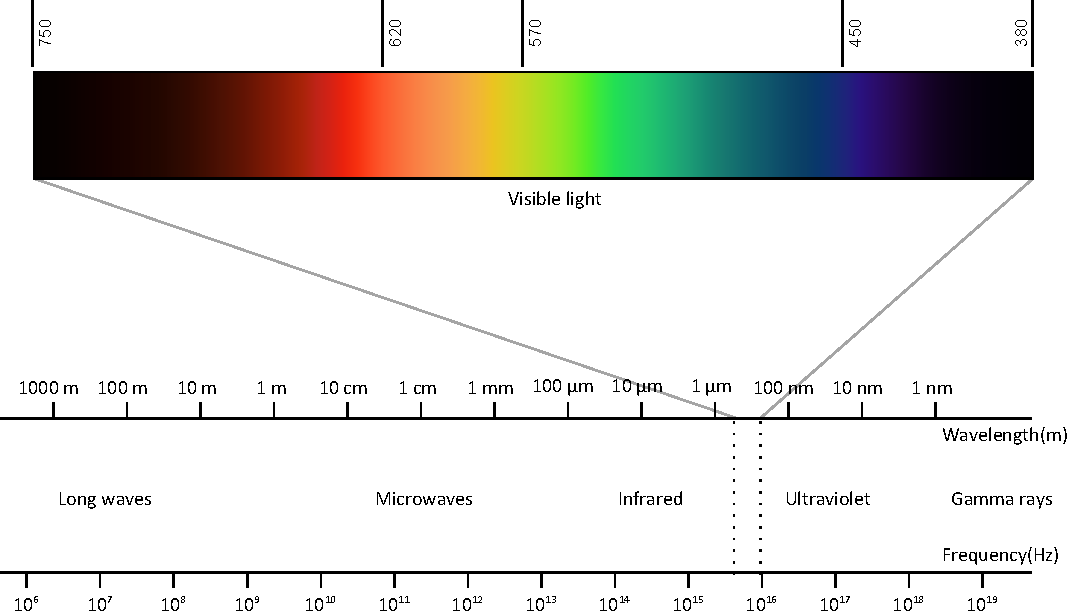
\includegraphics[width=1.0\textwidth]{images/spectrum.pdf}
\caption{The electromagnetic spectrum.}
\label{fig:spectrum}
\end{figure}

The branch of physics that studies how to measure electromagnetic radiation is called \emph{radiometry}. The energy of light, like all the others forms of energy, is measured in \emph{Joules} [\si{\joule} $=$ \si{\kg\meter\square\per\second\square}], and its power in \emph{Watts} [\si{\watt} $=$ \si{\kg\meter\square\per\second\cubed}]. \emph{Photometry}, on the other hand, measures electromagnetic radiation as it is perceived from the human eye, and limits itself only to the visible spectrum, while radiometry spans all of it. The corresponding names for energy and power in photometry are \emph{radiant energy}, measured in \emph{talbots} [\si{\candela\second}], and \emph{radiant flux}, measured in \emph{candelas} [\si{\candela}]. 

In image synthesis it is more common to use radiometry, as its quantities directly derive from the electromagnetic theories, are universal, and can be easily converted to the photometric ones when necessary. The most important radiometric quantities used in computer graphics are \emph{radiant flux}, \emph{radiant energy}, \emph{radiance}, \emph{irradiance} and \emph{intensity}.

\section{Radiometric quantities}

\subsection{Radiant flux}
The radiant flux, also known as radiant power, is the most basic quantity in radiometry. It is usually indicated with the letter $\Phi$ and it is measured in joules per seconds [\si{\joule\per\second}] or Watts [\si{\watt}]. The quantity indicates how much power the light irradiates per unit time. 

\subsection{Radiant energy}
Radiant energy, usually indicated as $Q$, is the energy that the light carries in a certain amount of time. Like all the other SI units for energy, it is measured in joules [\si{\joule}]. Radiant energy is obtained integrating the radiant flux along time for an interval $\Delta T$:

$$
Q = \int_{\Delta T} \Phi(t) \; dt
$$

Due to the dual nature of the light, the energy carried by the light can be derived both considering light as made of particles, called \emph{photons}, or considering it as a wave. We will not dig further into the topic, because for rendering purposes is not important if we characterize light as a flux of particles or as a sinusoidal wave.

\subsection{Irradiance}

Irradiance, usually defined as $E$, is the radiometric unit that measures the radiant flux per unit area \emph{falling} on a surface. It is measured in Watts per square meter [\si{\watt\per\square\meter}]. It is defined as the flux per unit area:
$$
E = \frac{d\Phi}{dA}
$$
Irradiance is usually the term in literature used for the \emph{incoming} power per unit area. The converse, i.e. the irradiance leaving a surface, it is usually referred as \emph{radiant exitance} or \emph{radiosity}, and indicated with the letter $B$.

\begin{figure}[!ht]
\centering
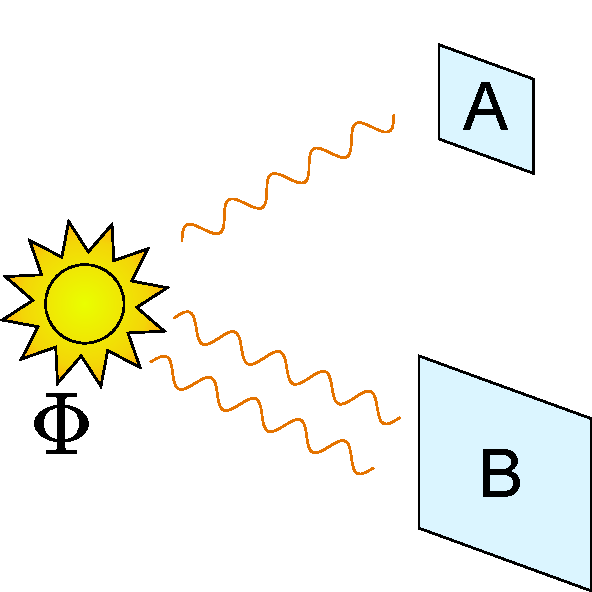
\includegraphics[width=0.5\textwidth]{images/irradiance.pdf}
\caption{Irradiance versus power. For the two surfaces $A$ and $B$, the received power $\Phi$ is the same, while the two irradiances $E_A$ and $E_B$ are different, as the area of $B$ is twice as the one of $A$.}
\label{fig:irradiance}
\end{figure}
 

\subsection{Intensity}
Intensity is defined as the differential radiant flux per differential solid angle:
\begin{equation}
I(\vomega) = \frac{d \Phi}{d \omega}
\label{eq:i}
\end{equation}
It is measured in Watts per steradian [\si{\watt\per\steradian}] and it is indicated with the letter $I$. Intensity is often a misused term in the physics community, as it is used for many different quantities. Depending on the research community, intensity may refer to irradiance or even to radiance (see the following section). The definition given in \ref{eq:i} we use the most common definition given by the optics community.

\subsection{Radiance}
Radiance is arguably the most important quantity in image synthesis. It is defined precisely as the differential of the flux per solid angle per projected surface area, and it is measured in Watt per steradian per square meter [\si{\watt\per\steradian\meter\square}].
$$
L(\vomega) = \frac{d^2 \Phi}{d\omega dA \cos \theta}
$$
Where $\theta$ is the angle between the surface normal and the incoming ray of light (so that $\cos\theta = \vec{n} \cdot \vomega_i$). 

\begin{figure}[!ht]
\centering
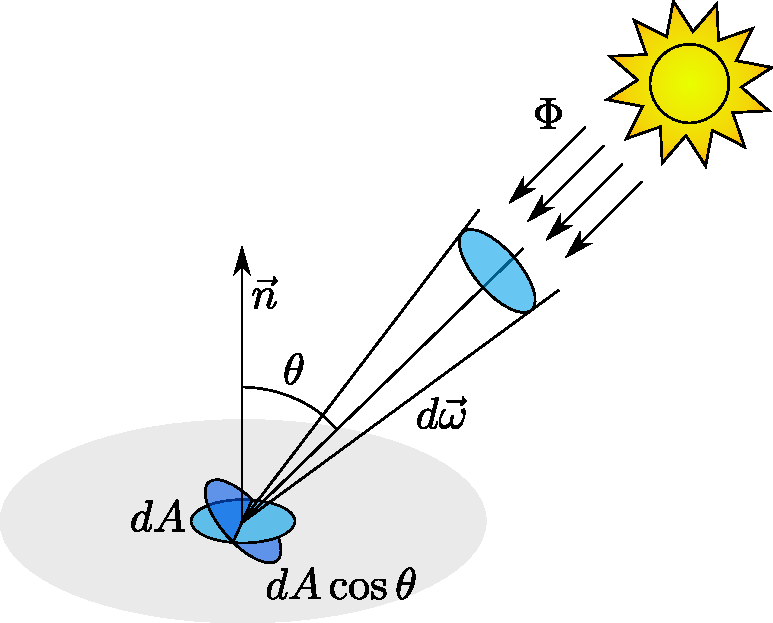
\includegraphics[width=0.7\textwidth]{images/radiance.pdf}
\caption{Radiance. The element of area $dA$ gets projected according to the angle $\theta = \cos^{-1}{\vec{n} \cdot \vomega}$. Then the incoming flux $\Phi$ gets divided by the projected area and by the solid angle subtended by it.}
\label{fig:radiance}
\end{figure}

Radiance has the important property of being constant along a ray of light. In addition, the sensibility of the human eye to light is directly proportional to the radiance. For a discussion on why radiance is related to the sensitivity of sensors and the human eye, see \cite{Cohen:1993:RRI:154731}.

All the other radiometric quantities can be derived from radiance:
\begin{equation}
\begin{split}
E &= \int_{2\pi} L_i(\vomega) \cos\theta \; d\omega \\
B &= \int_{2\pi} L_o(\vomega) \cos\theta \; d\omega \\
I(\vomega) &= \int_A L(\vomega) \cos\theta \; dA \\
\Phi &= \int_A \int_{2\pi} L(\vomega) \cos\theta \; d\omega dA
\end{split}
\label{eq:radiancederivation} 
\end{equation}
For simplicity of notation, the dependence from the point of incidence $\x$ has been dropped in equations \ref{eq:radiancederivation}. 

\subsection{Radiometric quantities for simple lights}

To help with the formulas used later in the report, we derive the standard radiometric quantities for the two simplest types of light, i.e. directional and point lights.
\begin{itemize}
	\item \textit{Directional lights} simulate very distant light sources, in which all the rays of light are parallel (e.g. sunlight). They are represented by a direction $\vomega_l$ and a constant radiance value, $L$. 
	\item \textit{Point lights} simulate lights closer to the observer. Isotropic point lights are represented by a position of the light $\x_l$ and a constant intensity $I$. Point lights have a falloff that depends on the inverse square law, i.e. the radiance diminishes with the square of the distance.
\end{itemize}

Table \ref{table:radio} shows different radiometric quantities evaluated for point and directional lights, for a surface point $\x$ with surface normal $\vec{n}$. 

\renewcommand{\arraystretch}{1.8}
\begin{table}[!ht]
    \centering
    \begin{tabularx}{0.95\textwidth}{|X|X|X|}
    \hline
    Quantity   & Directional light & Point light \\ \hline
    Cosine term       & $\cos\theta = \vec{n} \cdot \vomega_l$ & $\cos\theta = \frac{(\x - \x_l) \cdot \vec{n}}{|\x - \x_l|}$     \\ \hline
    $\Phi(\x)$ Flux       & $L\; \delta(\vec{\omega)}$                  & $4 \pi I$           \\ \hline
    $E(\x)$ Irradiance & $L \cos\theta $                 & $I \frac{\cos\theta}{|\x_l - \x|^2}$          \\ \hline
    $I(\x,\vomega)$ Intensity  & $L\; \delta(\vomega)$                 & $I$           \\ \hline
    $L(\x,\vomega)$ Radiance   & $L\; \delta(\vomega)$               & $\frac{I}{|\x_l - \x|^2}$           \\ \hline
    \end{tabularx}
\caption{Different radiometric values for simple light sources.}
\label{table:radio}
\end{table}

\section{Reflectance Functions}
After introducing the basic radiometric quantities, we still lack a way to describe light material interaction. More precisely, we need a way to relate the incoming and the outgoing radiance on a point of a chosen surface. 

\subsection{BRDF functions}
\label{sec:brdf}
One of the possible way to describe light-material interaction is by using a BDRF function \citep{Nicodemus:1992:GCN:136913.136929}, acronym for \emph{Bidirectional Reflectance Distribution Function}. The BRDF function $f(\x, \vomega_i, \vomega_o)$ is defined on one point $\x$ of the surface as the differential ratio between the exiting radiance and the irradiance:
\begin{equation}
f(\x, \vomega_i, \vomega_o) = \frac{d L_o(\x, \vomega_o)}{d E_i(\x, \vomega_i)} = \frac{d L_o(\x, \vomega_o)}{L_i(\x, \vomega_i) \cos\theta_i d \vomega_i}
\label{eq:brdf}
\end{equation}
The BRDF states that the incoming and the outgoing radiance are proportional, so that the energy hitting the material at the point $\x$ is proportional to the energy coming out from the point. BRDF functions have generally the following properties:
\begin{itemize}
	\item \emph{reciprocal}: for the Hemholtz reciprocity principle, a physics result that is also the basis of reverse path ray tracing \citep{Desolneux:2007:GTI:1557413}:
	$$
	f(\x, \vomega_i, \vomega_o) = f(\x, \vomega_o, \vomega_i)
	$$
	\item \emph{anisotropic}: if the surface changes orientation and $\vomega_i$ and $\vomega_o$ stays the same, the resulting BRDFs are different. So generally
	$$
	f(\x, \vomega_i, \vomega_o) \neq f(\x, R \vomega_o, R \vomega_i)
	$$
	where $R$ is a rotation matrix with arbitrary axis around the point $\x$.
	\item \emph{positive}, since the BRDF regulates the transport between two positive quantities (radiance, irradiance). 
	$$
	f(\x, \vomega_o, \vomega_i) \ge 0
	$$
	\item \emph{energy conserving}, so that the energy of the outgoing ray is no grater that the one of the incoming one 
	$$
	\int_{2\pi}  f(\x, \vomega_o, \vomega_i) \cos\theta_o d\vomega_o \le 1
	$$
\end{itemize}

By inverting equation \ref{eq:brdf}, we obtain the so-called \emph{reflectance equation}:
$$
L_o(\x, \vomega_o) = \int_{2\pi} f(\x, \vomega_i, \vomega_o) L_i(\x, \vomega_i) \cos\theta_i d\vomega_i
$$
Later we will use this equation as a starting point to obtain a formulation of the full rendering equation. The BRDF function has some limitations, being not able to account for all phenomena. For example, with a BRDF it is not possible to account for subsurface scattering, because it assumes the light enters and leaves the material at the same point. To model these phenomena, more complicated functions are needed, like the BSSRDF function described later in this chapter. 

\begin{figure}[!ht]
\centering
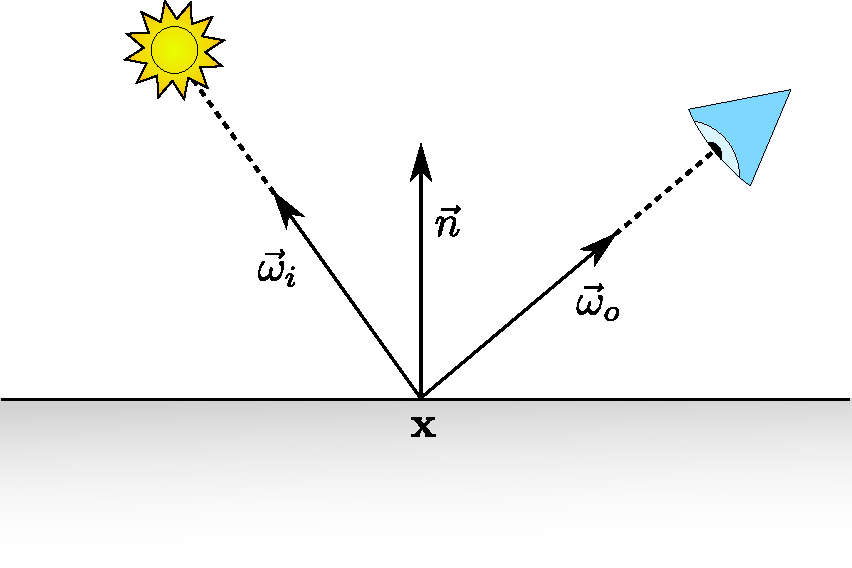
\includegraphics[width=0.8\textwidth]{images/brdf.pdf}
\caption{Setup for a BRDF. Note that the light enters and leaves the surface at the same point.}
\label{fig:brdf}
\end{figure}

\FloatBarrier 
\subsection{Examples of BRDF functions}
\begin{figure}
\centering
\subfloat[{Lambertian BRDF}]{
  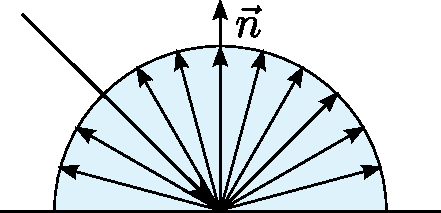
\includegraphics[width=0.4 \linewidth]{images/brdf_lambertian.pdf}
  \label{fig:lambertianbrdf}
}
\subfloat[{Mirror BRDF}]{
  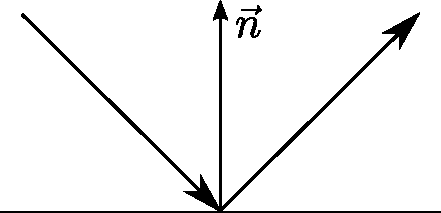
\includegraphics[width=0.4 \linewidth]{images/brdf_mirror.pdf}
  \label{fig:mirrorbrdf}
} \\
\subfloat[{Glossy BRDF}]{
  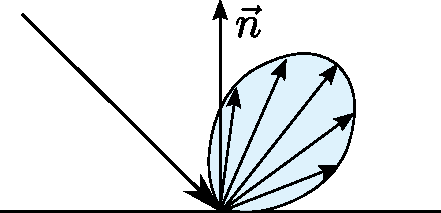
\includegraphics[width=0.4 \linewidth]{images/brdf_glossy.pdf}
  \label{fig:glossybrdf}
} 
\subfloat[{Combined BRDF}]{
  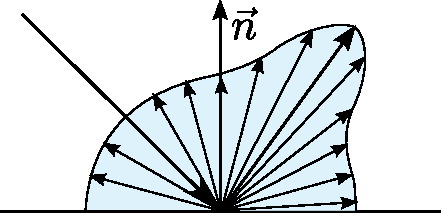
\includegraphics[width=0.4 \linewidth]{images/brdf_combined.pdf}
  \label{fig:combinedbrdf}
} 
\label{fig:brdfexamples}
\caption{Examples of BRDF functions. In this particular example, the three simple BRDFs can be evaluated separately and then combined in the more complex BRDF of Figure \ref{fig:combinedbrdf} in order to represent multiple effects.}
\end{figure}

There are many examples of BRDF functions in literature. In this section, in order to illustrate some examples, we will introduce three of them: the lambertian or diffuse BRDF, the specular or mirror BRDF and glossy BRDFs. For a detailed overview on BRDF functions, please refer to \citep{RTR3}.

\subsubsection{Lambertian BRDF}
In the lambertian BRDF, the incoming radiance is distributed equally in all directions, regardless of the incoming direction. To do this, the BRDF must be constant:
$$
f(\x, \vomega_i, \vomega_o) = k_d
$$
We can check that then the radiance is scattered equally in all directions by simple integration:

\begin{equation*}
\begin{split}
L_o(\x, \vomega_o) &= \int_{2\pi} f_d L_i(\x, \vomega_i) \cos\theta_i d\vomega_i \\
L_o(\x, \vomega_o) &= k_d \int_{2\pi} L_i(\x, \vomega_i) \cos\theta_i d\vomega_i \\
L_o(\x, \vomega_o) &= k_d \; E(\x) \\
\end{split}
\end{equation*}

The lambertian model is an ideal model, so very few material exhibit a lambertian diffusion, like unfinished wood or \emph{spectralon}, a synthetic material created in order to be as close as possible to a perfect lambertian material. Given its properties, spectralon is usually employed in calibrating radiance testing equipment. 

\subsubsection{Mirror BRDF}

Another simple kind of BRDF is the perfectly specular BRDF, or mirror BRDF. In this function, all the incoming radiance from one direction $\vomega_i$ is transferred towards the reflected direction $\vomega_r$, defined as $\vomega_r = \vomega_i - 2 (\vomega_i \cdot \vec{n}) \vec{n}$. The resulting BRDF is defined as follows:
$$
f(\x, \vomega_i, \vomega_o) = \frac{\delta(\vomega_o - \vomega_r)}{\cos\theta_i} 
$$
The function $\delta(\vomega)$ is a hemispheric delta function. Once integrated over a hemisphere, the function evaluates to one only for the vector $\vomega = \mathbf{0}$. Putting the BRDF into the reflectance equation gives the following outgoing radiance:
\begin{equation*}
L_o(\x, \vomega_o) = \begin{cases}
L_i(\x, \vomega_i)  &\text{if $\vomega_o = \vomega_r$}\\
0 &\text{otherwise}
\end{cases}
\end{equation*}
that is the expected result, as all the radiance is reflected into the direction $\vomega_r$.

\subsubsection{Glossy BRDFs}

As we can see from real life experience, rarely objects are completely diffuse or completely specular. These two models are idealized models, that represent an ideal case. So, to create a realistic BRDF model, we often need to combine the two terms and add an additional one, called glossy reflection.

The most used BRDF model used to model glossy reflections is based on microfacet theory \citep{Torrance:1992:TOR:136913.136924, Ashikmin:2000:MBG:344779.344814} and was first introduced by \citep{Blinn:1977:MLR:965141.563893}. In this theory, the surface of an object is modeled as composed of small mirrors. In one of its classical formulations, the BRDF is represented as:
$$
f(\x, \vomega_i, \vomega_o) = \frac{D G R}{4 \cos\theta_r \cos\theta_i} = \frac{G R}{4} \frac{(\vec{n}\cdot\vec{h})^s}{(\vec{n}\cdot\vec{r})(\vec{n}\cdot\vomega_i)}
$$
$D$ regulates how microfacets are distributed, and it is often modeled as $(\vec{n}\cdot\vec{h})^s$, where $\vec{h}$ is the half vector between the eye and the light, and $s$ is an attenuation parameter. $\vec{h}$ is defined as:
$$
\vec{h} = \frac{\vomega_o + \vomega_i}{\left\| \vomega_o + \vomega_i \right\|}
$$
$G$ accounts for the object self shadowing, while $R$ is the Fresnel reflection term (more details in Section \ref{sec:fresnel}).	$\vec{r}$ is the reflection vector as defined in the previous section. See Figure \ref{fig:glossysetup} on how the vectors for the glossy reflection - $\vec{n}$, $\vec{h}$ and $\vec{r}$ - are defined.


\begin{figure}[!ht]
\centering
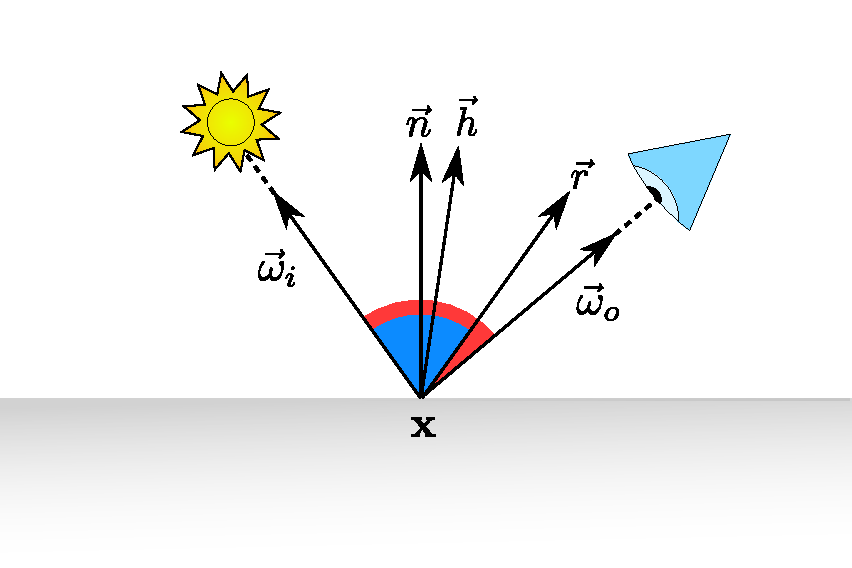
\includegraphics[width=0.7\textwidth]{images/glossy_setup.pdf}
\caption{Glossy vectors for microfacet theory. The blue angles are the same for the reflection vector, the red ones are the same for the half vector.}
\label{fig:glossysetup}
\end{figure}
 
Various alternative definitions exist for the $D$ and $G$ function, varying among the literature. Other glossy models not based on microfacet theory do exist as well \citep{RTR3}. 

\subsection{The rendering equation}

Given the reflectance equation, it is possible to generalize it in order to model all the lighting in an environment (global illumination). In fact, the described reflectance equation is a suitable candidate to represent a full global illumination equation, but it does not account for two important factors. 

The first factor are emissive surfaces. We need to add an emissive radiance term $L_e(\x, \vomega)$ that models the amount of radiance that a point is emitting in a certain direction. This is useful to model light sources, without introducing a separate equation. We note that point lights have a singularity: they emit infinite radiance on the point where they are placed.

The second factor is that the reflectance equation accounts only for direct illumination. In general, we want to include also light that bounced onto another surface before reaching the current surface. To model this, we can replace the $L_i$ term in the reflectance equation with another term $L_r$ that accounts for light coming from another surface. This term can be usually modeled as the product of the radiance of the light plus a visibility function $V(\x)$.

Accounting for all the described factors, we reach one formulation of the rendering equation \citep{Kajiya:1986:RE:15886.15902}:
$$
L_o(\x, \vomega_o) = L_e(\x, \vomega) + \int_{2\pi} f(\x, \vomega_i, \vomega_o) L_i(\x, \vomega_i) V(\x) \cos\theta_i d\vomega_i
$$
This form of the rendering equation is still not completely general, since it is based on a BRDF, to it comes with the same limitations (no subsurface scattering effects or wavelength-changing effects like iridescence). We will extend the rendering equation in order to account for these phenomena later on in this chapter.

\subsection{Fresnel equations}
\label{sec:fresnel}

Until now, on the described BRDF models, we did consider only the reflected part of the radiance. When a beam of light coming from direction $\vomega_i$ hits a surface, only part of the incoming radiance gets reflected, while another part gets refracted into the material. As we can see from Figure \ref{fig:fresnelsetup}, we obtain the two vectors $\vomega_r$ and $\vomega_t$, the reflected and refracted vector, defined as follows \citep{Kay:1979:TCS:965103.807438}:
\begin{equation*}
\begin{split}
\vomega_r &= \vomega_i - 2 (\vomega_i \cdot \vec{n}) \vec{n} \\
\vomega_t &= \eta ((\vomega_i \cdot \vec{n}) \vec{n} - \vomega_i) - \vec{n} \sqrt{1 - \eta^2 (1 - (\vomega_i \cdot \vec{n}) ^ 2)}
\end{split}
\end{equation*}
\begin{figure}[!ht]
\centering
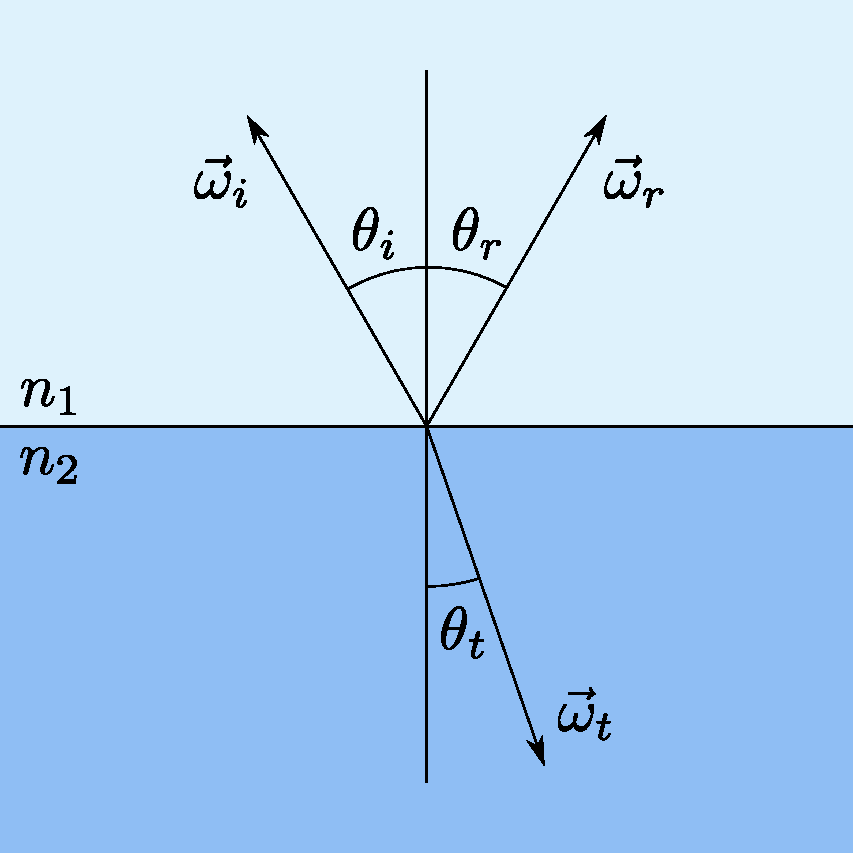
\includegraphics[width=0.5\textwidth]{images/fresnelsetup.pdf}
\caption{Reflected and refracted vector on mismatching indices of refraction.}
\label{fig:fresnelsetup}
\end{figure}
Where $\eta = \frac{n_1}{n_2}$ is the relative index of refraction between the two materials. With this setup, illustrated in Figure \ref{fig:fresnelsetup}, we can use a solution to Maxwell's equations for wave propagation to describe the radiant flux. In particular, we can tell which part of the power propagates in the reflected and refracted direction respectively. The coefficients that describe this subdivision of the power are called \emph{Fresnel coefficients} \citep{ob:bornwolf}. The coefficients are different according to the polarization of the incoming light (parallel or perpendicular), so there are two for reflection ($R_s$, $R_p$) and two for transmission ($T_s$, $T_p$).
\begin{equation*}
\begin{split}
R_s(\eta,\vomega_i) &= \left|\frac{\eta \cos\theta_i - \cos\theta_t} {\eta \cos\theta_i + \cos\theta_t}\right|^2 \\
R_p(\eta,\vomega_i) &= \left|\frac{\eta \cos\theta_t - \cos\theta_i} {\eta \cos\theta_t + \cos\theta_i}\right|^2\\
T_s(\eta,\vomega_i) &= \eta \ \frac{ \cos\theta_t}{ \cos\theta_i} \left|\frac{2 \cos\theta_i}{\eta \cos\theta_i + \cos\theta_t}\right|^2 \\
T_p(\eta,\vomega_i) &= \eta \ \frac{ \cos\theta_t}{ \cos\theta_i} \left|\frac{2 \cos\theta_i}{\eta \cos\theta_t + \cos\theta_i}\right|^2
\end{split}
\end{equation*}
In most computer graphics applications (and this is reasonable for most of the real-world lights), we assume that the two polarizations are equally mixed. So, we will use the coefficient $R = \frac{R_s + R_p}{2}$ and $T = \frac{T_s + T_p}{2}$ in our calculations. Note that $R + T = 1$, so the overall energy is conserved.

\subsection{BSSRDF functions and generalized rendering equation}
\begin{figure}
\centering
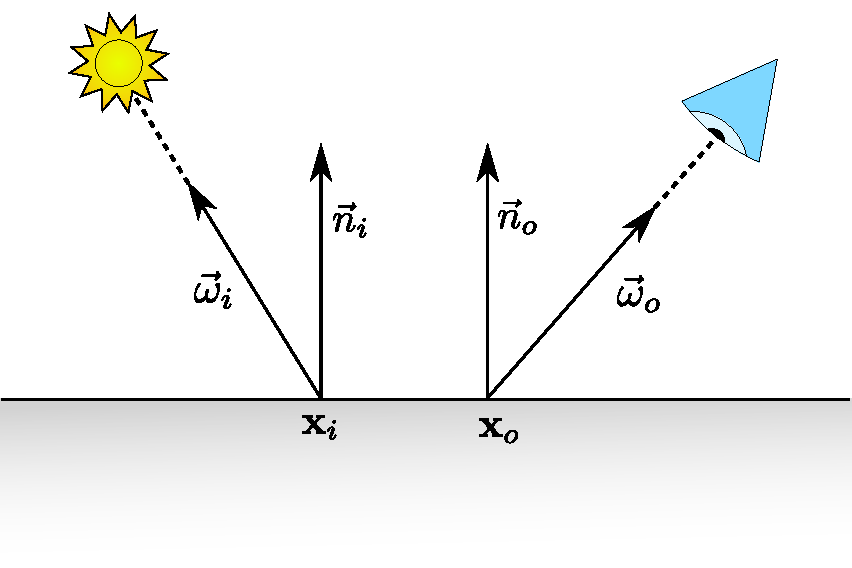
\includegraphics[width=0.8 \linewidth]{images/bssrdf} 
\caption{BSSRDF setup. As we compare it to the one of Figure \ref{fig:brdf}, we can see that the light enters and leaves the surface at two different points.}
\label{fig:bssrdf}
\end{figure}

As we anticipated in Section \ref{sec:brdf}, the BRDF theory that was introduced before is not accurate in predicting the behavior for all materials, since BRDF models assume that the light enters and leaves the material in the same point. While this assumption holds true for a wide range of material, like metal or plastic, it poorly describes translucent materials, that exhibit a consistent amount of light transport under the surface. 

In order to describe light transport in this material, we introduce a function, called BSSRDF \citep{Nicodemus:1992:GCN:136913.136929}, acronym for \emph{Bidirectional Subsurface Scattering Reflectance Distribution Function}. This function extends the concept of BRDF to account for two separate points. The BSSRDF is usually indicated with a capital $S$. We define the BRDF as the ratio between the incoming flux in a point $\x_i$ from the direction $\vomega_i$ and the outgoing radiance in \emph{another} point $\x_o$ on direction $\vomega_o$:
$$
S(\x_i, \vomega_i, \x_o, \vomega_o) = \frac{d L_o(\x_o,\vomega_o)}{d \Phi_i(\x_i,\vomega_i)} = \frac{d L_o(\x_o,\vomega_o)}{d E_i(\x_i,\vomega_i) d A_i} = \frac{d L_o(\x_o,\vomega_o)}{L_i(\x_i,\vomega_i) \cos \theta_i d\vomega_i d A_i}  
$$
As we can see, the BSSRDF is similar to the BRDF, apart from a additional derivation in the area domain. Once we rearrange this equation, we can obtain an updated reflectance equation for the BSSRDF:
$$
L_o(\x_o,\vomega_o) = \int_A \int_{2\pi} S(\x_i, \vomega_i, \x_o, \vomega_o) L_i(\x_i,\vomega_i) \cos \theta_i d\vomega_i d A_i
$$
We can immediately see that the new reflectance equation accounts for light scattering between two points, but this generality comes with a price. In fact, it adds a order of magnitude of complexity, since now the BSSRDF needs to be integrated twice, once on the whole surface and once on the normal hemisphere.

As we did for the BRDF, we can further extend the reflectance equation to further include visibility and emission, giving an extended form of the rendering equation \citep{Jensen:2001:PMS:383259.383319}. 
\begin{equation}
L_o(\x_o,\vomega_o) = L_e(\x_i,\vomega_i) + \int_A \int_{2\pi} S(\x_i, \vomega_i, \x_o, \vomega_o) L_i(\x_i,\vomega_i) V(\x) (\vec{n} \cdot \vomega_i) d\vomega_i d A_i
\label{eq:bssrdfeq}
\end{equation}
From now on, by `rendering equation' in this report we will mean the one in equation \ref{eq:bssrdfeq}. 

\section{Light transport and subsurface scattering}
\FloatBarrier
\begin{figure}
\centering
\subfloat[{Emission}]{
  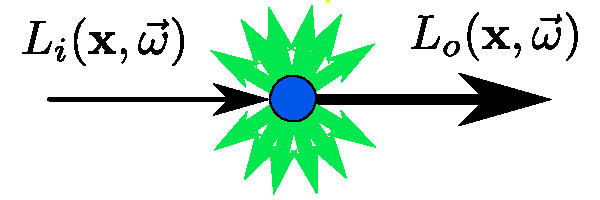
\includegraphics[width=0.5 \linewidth]{images/transport_emission.pdf}
  \label{fig:emission}
}
\subfloat[{Absorption}]{
  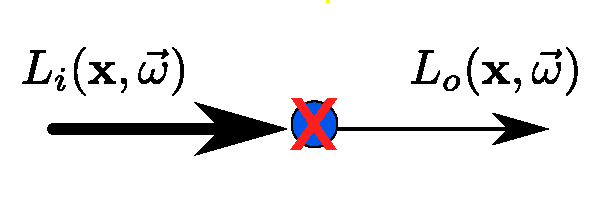
\includegraphics[width=0.5 \linewidth]{images/transport_absorption.pdf}
  \label{fig:absorption}
} \\
\subfloat[{Out Scattering}]{
  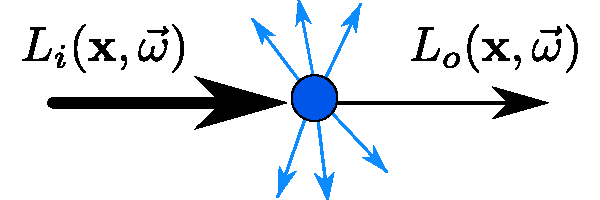
\includegraphics[width=0.5 \linewidth]{images/transport_outscattering.pdf}
  \label{fig:outscattering}
} 
\subfloat[{In Scattering}]{
  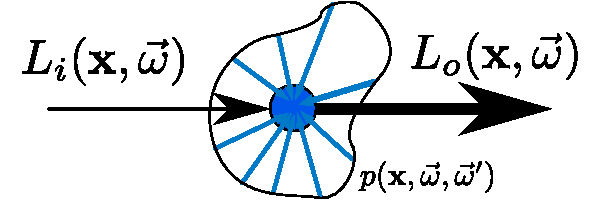
\includegraphics[width=0.5 \linewidth]{images/transport_inscattering.pdf}
  \label{fig:inscattering}
} 
\label{fig:transport}
\end{figure}

When we derive our models for lighting, in general we assume that the light is traveling in vacuum. This assumption holds for light that is propagating though the air (which is assimilable to vacuum), but once we relax it, more variables should be taken into consideration. Objects through which light travels are referred as \emph{participating media}. In this chapter, we will derive and consider an alternative formulation of the rendering equation for light traveling into participating media, called \emph{radiative transfer equation} \citep{Chandrasekar:1950:RT}.

When a beam of light travels through an object, various phenomena occur. A photon on the beam can be either being absorbed (disappear), scattered (change direction) or emitted (appear). These phenomena can be uniform throughout the material (homogeneous materials), as in solid materials like wax or leaves, or be not uniform (heterogeneous materials), like in smoke or clouds.

We will briefly describe all three mentioned effects, then combine them to compose the radiative transfer equation. The purpose is to describe how radiance varies along a beam of light with direction $\vomega$. This directional derivative is indicated as:
$$
(\vec{\nabla} \cdot \vomega) L(\x, \vomega) = \frac{\partial L_x}{\partial x} \vomega_x + \frac{\partial L_y}{\partial y} \vomega_y + \frac{\partial L_z}{\partial z} \vomega_z
$$ 

\subsection{Emission}
Emission is the natural property of the materials to emit light, i.e. to generate photons that add to the existing ones passing through the material. The effect is generally generated by chemical processes emitting photons (as in fireflies), by natural black-body radiation emission in the visible spectrum (such as in a star like the sun or in incandescent bulbs), or by other radiation that changes its wavelength into the visible spectrum.

In the directional 3D derivative, the variance in emission is modeled as a constant depending only on the current position and direction:
$$
(\vec{\nabla} \cdot \vomega) L(\x, \vomega) = \epsilon(\x, \vomega)
$$
This means that emission increases linearly along the body: if the beam travels a distance $d$ within the medium, $d \cdot k$ photons are emitted. Emission is generally isotropic, not depending on the direction ($ \epsilon(\x, \vomega) =  \epsilon(\x)$).

\subsection{Absorption}
Absorption is a property of materials that describes a simple physical phenomenon: a photon, traveling though the material, hits one atom of the material. The energy carried by the photon is then absorbed by the atom, augmenting its kinetic energy. This directly translates in an increase of heat in the material. Usually, a certain percentage of the photons that hit the atoms is absorbed per unit length. Then, if $k$ is the percentage of the photons absorbed in a meter, after one meter the original radiance will become $k \cdot L_i$, then $k^2 \cdot L_i$, etc.

If we write this phenomena as a differential equation, we get after a distance $d$ a radiance reduction of $k^d = e^{-\sigma_a d}$, that leads to the following 3D directional derivative:
$$
(\vec{\nabla} \cdot \vomega) L(\x, \vomega) = -\sigma_a(\x,\vomega) L(\x, \vomega)
$$
$\sigma_a$ is referred as the \emph{absorption coefficient}. Also this coefficient is generically isotropic, and constant for homogenous materials.

\subsection{Out-scattering}
Out scattering is the radiance lost due to scattering. The scattering phenomenon happens when photons are deflected away from the current direction $\vomega$.  As in the previous case, the phenomena is modeled as a percentage of the radiance lost per unit length. So the loss due to out-scattering is modeled as:
$$
(\vec{\nabla} \cdot \vomega) L(\x, \vomega) = -\sigma_s(\x,\vomega) L(\x, \vomega)
$$
$\sigma_s$ is referred as the \emph{scattering coefficient}. We note that in this case we are not interested in which direction the photons are actually going. That will be accounted in the in-scattering term of another point in the material.

\subsection{In-scattering}
Given some loss due to some of the photons changing direction, there will be some of them that from other scattering events will change to the $\vomega$ direction. We need then to discover the number of photons that comes from all the other directions. To do this, we integrate the incoming radiance from all directions in the point $\x$. This quantity, similar to irradiance, in an infinite medium is called \emph{fluence}, and indicated as $\phi$:
$$
\phi(\x) = \int_{4\pi} L(\x,\vomega') d\omega'
$$
Fluence should be then averaged over the entire sphere, yielding $\frac{\phi}{4\pi}$ as a normalization factor. This quantity then is then multiplied by the scattering coefficient, because only some photons on average scatter towards the current point. This results in:
\begin{equation}
(\vec{\nabla} \cdot \vomega) L(\x, \vomega) = \sigma_s(\x) \frac{1}{4 \pi} \int_{4\pi} L(\x,\vomega') d\omega'	
\label{eq:inscatter}
\end{equation}
However, equation \ref{eq:inscatter} assumes that radiance scatters equally in all directions. This is not usually the case, and the $\frac{1}{4 \pi}$ term needs to be replaced by a probability distribution function that describes how the photons scatter in the medium. This function is called \emph{phase function}, and indicated as $p(\x, \vomega, \vomega')$. In the actual models its integral on the hemisphere is often used as a parameter, called \emph{mean cosine} ($g$):
$$
g(\x) = \int_{4 \pi} p(\x, \vomega, \vomega') \vomega \cdot \vomega' d \omega'
$$
This term indicates the general direction of the scattering in the material. If positive, the scattering is prevalent along the beam (forward scattering), if negative is prevalent in the opposite direction (backward scattering). If zero, the scattering is isotropic, i.e. equal in all directions.

So, the final 3D equation for in-scattering, accounting for the phase function, is as follows:
\begin{equation*}
(\vec{\nabla} \cdot \vomega) L(\x, \vomega) = \sigma_s(\x) \int_{4\pi} p(\x, \vomega, \vomega') L(\x,\vomega') d\omega'	
\end{equation*}

\subsection{Final formulation of the radiative transfer equation}
Combining emission, absorption, scattering described in the previous sections, we reach the final formulation of the radiative transfer equation (RTE):
\begin{equation}
(\vec{\nabla} \cdot \vomega) L(\x, \vomega) =   -\sigma_t(\x) L(\x, \vomega) + \epsilon(\x) + \sigma_s(\x) \int_{4\pi} p(\x, \vomega, \vomega') L(\x,\vomega') d\omega'
\label{eq:rte}
\end{equation}
Where the two reducing term, scattering and absorption, have been combined together in $\sigma_t = \sigma_a + \sigma_s$, called the \emph{extinction coefficient}.


\subsection{The diffusion approximation}
The radiative transfer equation \ref{eq:rte} is a integro-differential equation with many degrees of freedom. As we stated in Chapter \ref{chap:previous}, there are rendering techniques that numerically solve the equation in order to obtain a realistic result. However, analytical methods tend to use some approximations of the RTE, that hold well given specific conditions. The \emph{diffusion approximation} \citep{books/daglib/0093591} is one of these approximations, and it is still widely used today since its introduction in the computer graphics community by \citep{raey}. 

The assumption under the diffusion approximation is that given a physical medium, the number of scattering events is so high that the beam of light quickly becomes isotropic. Each one of the scattering events blurs the light distribution, and as a result the distribution becomes more uniform as the number of scattering events increases. This has been proven to be a reasonable assumption even for highly anisotropic light sources (e.g. a focused laser beam) and phase functions.

When using the diffusion approximation, instead of using the extinction coefficient $\sigma_t$, we account for the contribution from the phase function by using the so-called \emph{reduced extinction coefficient} $\sigma_t'$. It is defined as $\sigma_t' = \sigma_a + \sigma_s'$, with $\sigma_s' = \sigma_s (1 - g)$. $\sigma_s'$ Is called \emph{reduced scattering coefficient}. The converse of the reduced extinction coefficient is called \emph{mean free path} and represents the average distance that light travels in the medium before being absorbed or scattered.

The rationale behind this reduced coefficient is that a highly forward scattering material is virtually indistinguishable from a not-scattering material. So, for highly forward scattering materials ($g \approx 1$) the scattering coefficients reduce to zero. For highly backward scattering materials ($g \approx -1$), the scattering is accounted for twice as for an isotropic material (see table \ref{table:coefficients}).

\renewcommand{\arraystretch}{1.8}
\begin{table}[!ht]
    \centering
    \begin{tabularx}{0.95\textwidth}{|X|X|X|X|}
    \hline
    Coefficient   & Backward\linebreak Scattering \linebreak $(g \approx -1)$ & Isotropic \linebreak\linebreak $(g \approx 0)$ & Forward \linebreak Scattering \linebreak $(g \approx 1)$ \\ \hline
    $\sigma_s'$   & $2 \sigma_s$ & $\sigma_s$ & 0   \\ \hline
    $\sigma_t'$   & $\sigma_a + 2 \sigma_s$ & $\sigma_a + \sigma_s$ &  $\sigma_a$  \\ \hline
    \end{tabularx}
\caption{Explicit scattering coefficients for different kinds of materials.}
\label{table:coefficients}
\end{table}

We leave to \cite{books/daglib/0093591} and \cite{Jensen:2001:PMS:383259.383319} for the algebraic details of the calculation. Once we solve the diffusion equation, we obtain the following formula for $\phi(\x)$, the fluence of light in an infinite scattering medium.
\begin{equation}
\phi(\x) = \frac{\Phi}{4\pi D} \frac{e^{\sigma_{tr} r}}{r}
\label{eq:dasimple}
\end{equation}
We recall that $\phi(\x) = \int_{4\pi}L(\x,\vomega) d\vomega$. $r = \|\x\|$ is the distance from the point to the light source. The two coefficients $D$ and $\sigma_{tr}$ are called \emph{diffusion coefficient} and \emph{transmission coefficient} respectively. The two coefficients are defined as follows:
\begin{equation*}
\begin{split}
D &= \frac{1}{3 \sigma_t'} \\
\sigma_{tr} &= \sqrt{3 \sigma_a \sigma_t'} = \sqrt{\frac{\sigma_a}{D}}
\end{split}
\end{equation*}
This is the equation describe light propagation in an infinite medium, i.e. no surface interaction is considered. In order to derive an actual BSSRDF model from the diffusion approximation, \emph{boundary conditions} must be considered. Jensen \cite{Jensen:2001:PMS:383259.383319} derived an analytical model starting from this approximation of the RTE, while Frisvad \cite{IMM2013-06646} uses a higher order diffusion approximation of the RTE. The two models are explained in the following sections.

\subsection{Standard dipole model}
 
The first model we describe is due to \cite{Jensen:2001:PMS:383259.383319}. It it usually referred in literature as \emph{Jensen dipole model} or \emph{Standard dipole model}. In their original paper, the authors used the diffusion approximation for light in an infinite medium. Starting from that, they derive an approximation that holds for light in a semi-infinite medium, i.e. light traveling in void hitting a planar slab of a translucent material.

As a boundary condition, we take the light coming \emph{out} of the material. Light coming out of the material has a initial fluence $\phi_0$. We assume then that the fluence decays linearly until a distance $z = 2 A D$ from the surface, where it becomes zero. See \cite{Donner:2006:TRI:1236937} for the full derivation. $D$ is the diffusion coefficient, while $A$ is a corrective term that accounts for mismatching indices of refraction:
\begin{equation}
\begin{split}
A &= \frac{1 + F_{dr}}{1 - F_{dr}} \\
F_{dr} &= \int_{2\pi} R(\eta, \vec{n} \cdot \vomega)  (\vec{n} \cdot \vomega) d \vomega
\end{split}
\end{equation}
Where $R$ is the Fresnel reflection term as defined in Section \ref{sec:fresnel}, and $\eta = n_1 / n_2$ is the relative refraction index. The Fresnel reflectance integral $F_{dr}$ is usually approximated with an analytical expression:
$$
F_{dr} = -\frac{1.440}{\eta^2} + \frac{0.710}{\eta} + 0.668 + 0.0036 \eta
$$
Given the boundary condition, we can then model the subsurface scattering in a point $\x_o$ with two small sources on the point, a configuration called a \emph{dipole}. One source is placed beneath the surface, called the \emph{real source}, while the other one is mirrored above the surface, called \emph{virtual source}. The first source actually models the subsurface scattering effect, while the second one reduces the first in order to account for the boundary conditions and the extrapolation boundary. Refer to Figure \ref{fig:jensen} for a visual detail on the setup.

\begin{figure}[!ht]
\centering
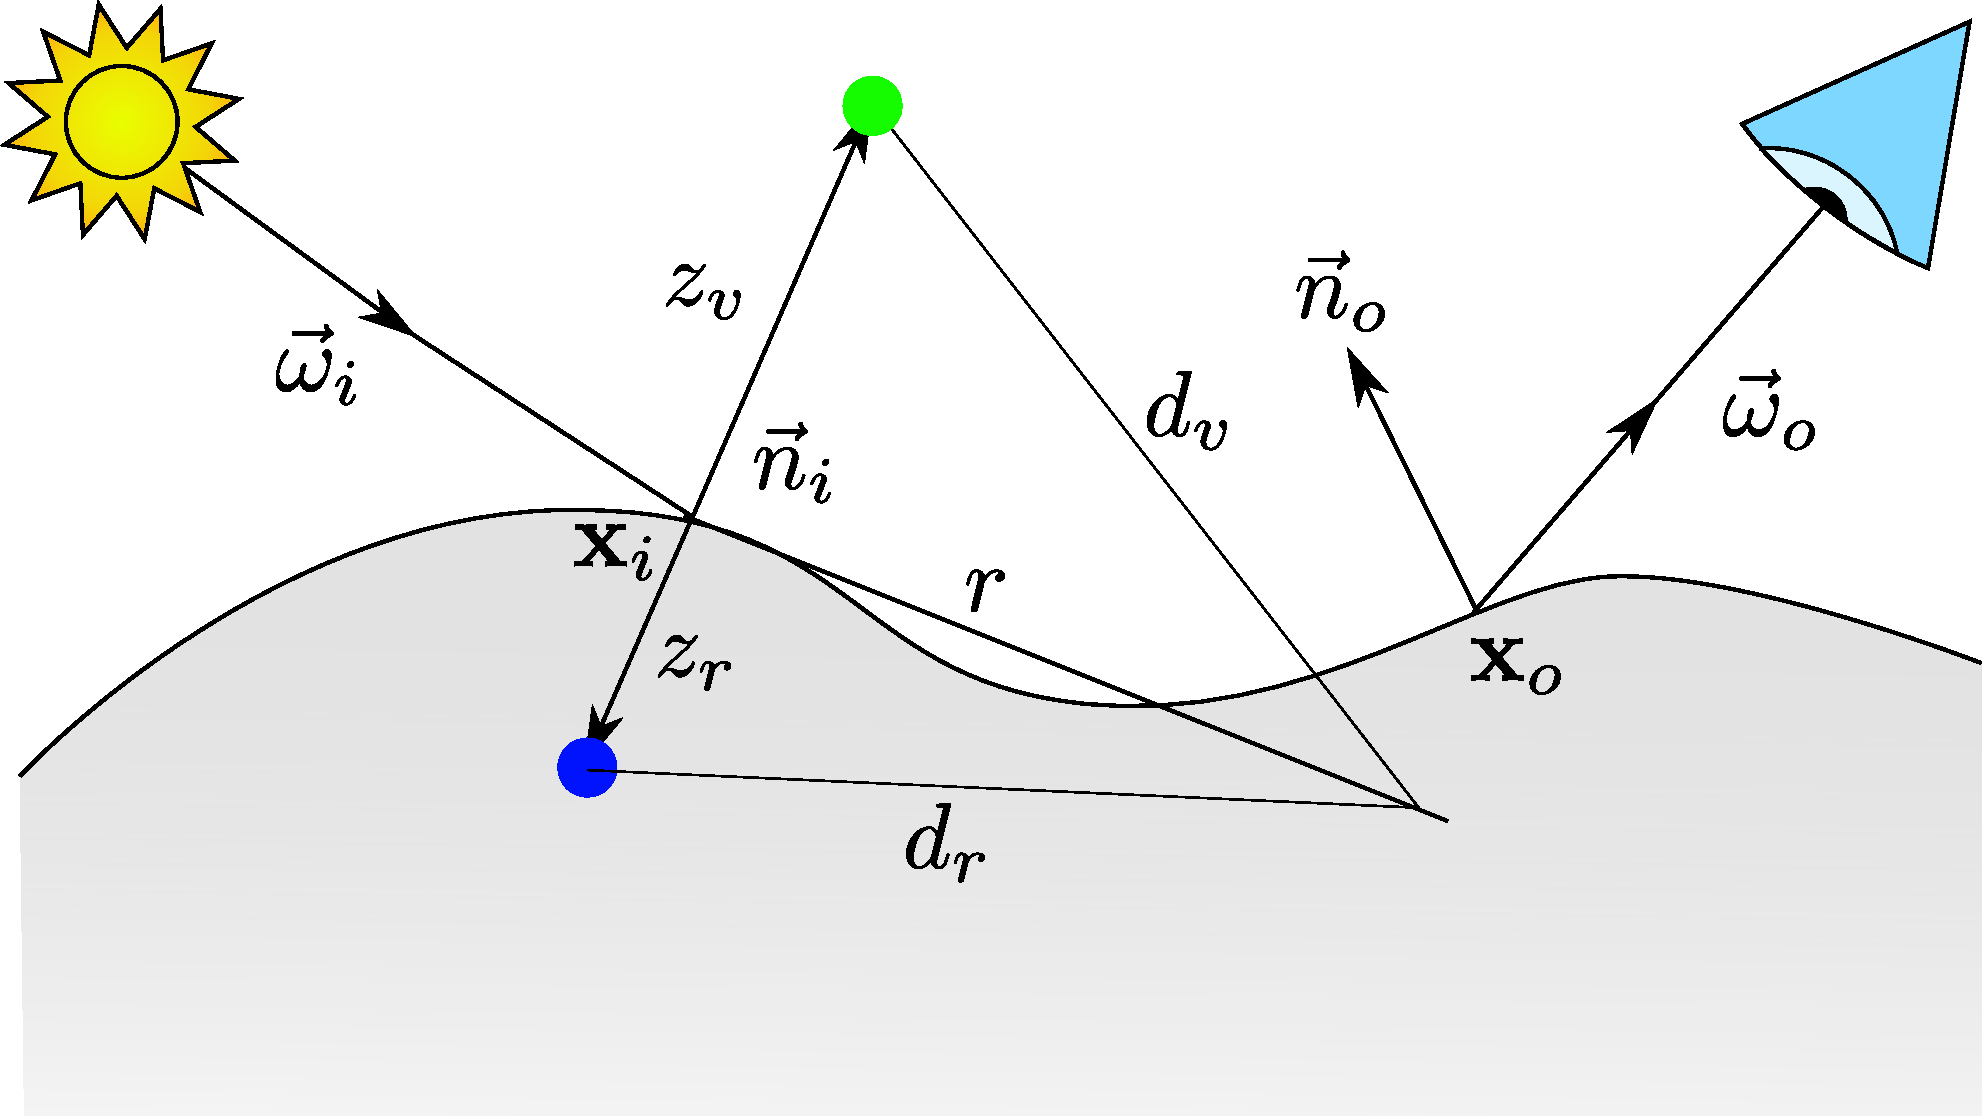
\includegraphics[width=\textwidth]{images/jensen.pdf}
\caption{Setup for the standard dipole model.}
\label{fig:jensen}
\end{figure}

The real source is placed one mean free path beneath the surface, at $z_r = 1 / \sigma_t'$, while the virtual one is placed symmetrically according to the boundary conditions, ad a distance $z_v = z_r + 4 A D$. From $z_r$ and $z_v$ we can calculate the distances $d_r$ and $d_v$ from the entrance point $\x_i$. Given $r = \|\x_o -\x_i\|$, we obtain:
\begin{equation*}
\begin{split}
d_r &= \sqrt{z_r^2 + r^2} \\
d_v &= \sqrt{z_v^2 + r^2}
\end{split}
\end{equation*}
Given these constraints, we obtain an equation for the BSSRDF in a semi infinite medium:
$$
S_d(\x_i,\vomega_i,\x_i,\vomega_o) = \frac{\alpha'}{4 \pi^2} \left[\frac{z_r (1 + \sigma_{tr} d_r) \; e^{-\sigma_{tr} d_r}}{d_r^3} + \frac{z_v (1 + \sigma_{tr} d_v) \; e^{-\sigma_{tr} d_v}}{d_v^3} \right]
$$
Where $\alpha' = \sigma_s' / \sigma_t'$ is called \emph{reduced albedo}.

The model so far described was intended to model only the multiple scattering BSSRDF term, $S_d$. In order to obtain the full BSSRDF $S$, a single scattering term $S^{(1)}$ must be added. Moreover, we need to add as well the two Fresnel transmission terms, one for the incoming and one for the outgoing radiance. There are in literature many approaches to model single scattering, that are out of the scope of this report. The final BSSRDF equation for the standard dipole model then becomes:
$$
S(\x_i, \vomega_i, \x_o, \vomega_o) = T(\eta,\vomega_i) S_d(\x_i, \vomega_i, \x_o, \vomega_o) T(\eta,\vomega_o) + S^{(1)}(\x_i, \vomega_i, \x_o, \vomega_o)
$$
\cite{Jensen:2001:PMS:383259.383319} in their original paper describes some corrections that need to be done to the model in order to make it work with generic surfaces, and on how to account for extensions like texture support. We will not describe these extensions here, remanding to the original paper for a detailed description.

\subsection{Directional dipole model}
 
Various evolutions to the standard dipole model have been proposed throughout the years. In this chapter, we will introduce the BSSRDF approximation called \emph{directional dipole}, proposed by \cite{IMM2013-06646}. In the standard dipole model, in fact, the diffusive part of the BSSRDF depends only on the distance between the point of incidence and the point of emergence, that is $S_d(\x_i, \vomega_i, \x_o, \vomega_o) = S_d(\|\x_o - \x_i\|)$. 

The directional dipole model, based on the diffusion approximation, accounts for the direction of the incoming light in its calculations, in order to model the scattering effects more precisely. Moreover, the model, instead of splitting the BSSRDF in a multiple and single scattering term, splits the BSSRDF into a diffusive term $S_d$ and a term $S_{\delta E}$, called \emph{reduced intensity}, that can be computed using the delta-Eddington approximation\cite{delta}. The final BSSRDF thus becomes:
\begin{equation}
S(\x_i, \vomega_i, \x_o, \vomega_o) = T(\eta,\vomega_i) (S_d(\x_i, \vomega_i, \x_o) + S_{\delta E}(\x_i, \vomega_i, \x_o, \vomega_o)) T(\eta,\vomega_o)
\label{eq:bssrdfgen}
\end{equation}
Where $T$ are the Fresnel transmission coefficients for the incoming and outgoing directions. We note also that the diffusive part of the BSSRDF does not depend on the outgoing direction $\vomega_o$. 

\textbf{Diffusive BSSRDF}
The diffusive part of the directional dipole model uses a first-order approximation of the RTE, that for a point light in an infinite medium gives the following fluence:
\begin{equation}
\phi(\x_o, \theta) = \frac{\Phi}{4\pi D} \frac{e^{\sigma_{tr} r}}{r} \left( 1 + 3D\frac{1 + \sigma_{tr} r}{r}\cos\theta\right)
\label{eq:daa}
\end{equation}
Where $D$ and $\sigma_{tr}$ are the two scattering coefficients defined beforehand, $r = \|\x_o\|$ and 
$$
\cos \theta = \frac{\x \cdot \vomega_{12}}{r}
$$
Where $\vomega_{12}$ is the refracted vector as defined in Section \ref{sec:fresnel}. Comparing \ref{eq:daa} with equation \ref{eq:dasimple}, we can see that we introduced a new term that depends on the angle $\theta$ between the refracted incoming light vector and the vector connecting incidence and emergence. 

\begin{figure}[!ht]
\centering
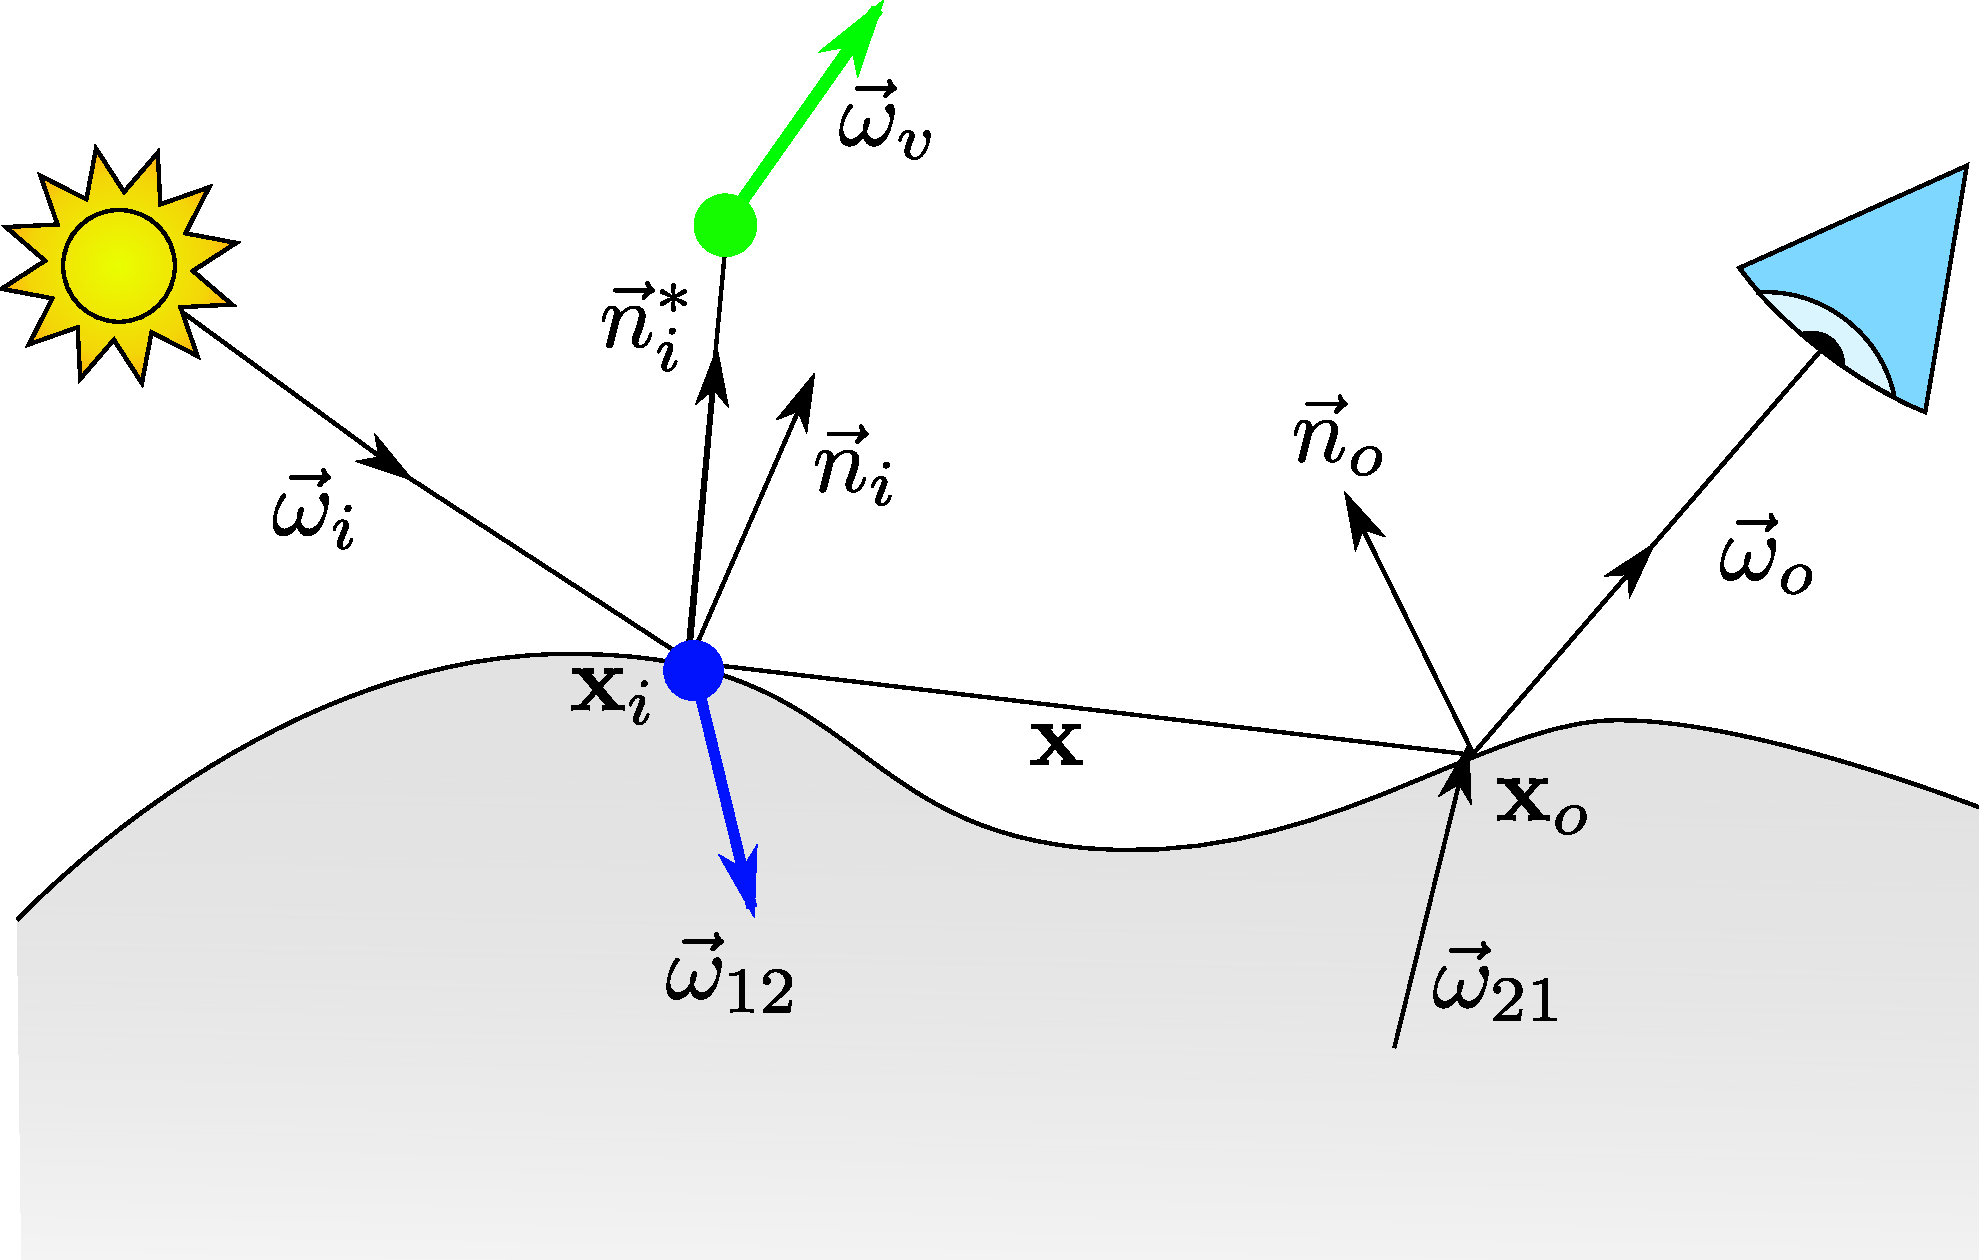
\includegraphics[width=0.9\textwidth]{images/jeppe.pdf}
\caption{Setup for the directional dipole model.}
\label{fig:jeppe}
\end{figure}

Using the diffusion approximation, we can first establish a relationship between the radiant exitance $M(\x_o)$ and the diffusive BSSRDF $S'_d$ in an infinite medium:
\begin{equation}
\frac{d M(\x_o)}{d \Phi_i(\x, \vomega_i)} = T(\eta, \vomega_i) S'_d(\x_i, \vomega_i, \x_o) \; 4\pi\csinv 
\label{eq:m2}
\end{equation}
Where $\csinv$ is related to the integral on the hemisphere of the fresnel coefficients. Using the definition of radiant exitance and inserting inside the classical diffusion approximation, we reach the diffusion formulation of the radiant exitance:
\begin{equation}
M(\x_o) = \cs \phi(\x_o) + \ce D \vec{n}_o \cdot \nabla \phi(\x_o)
\label{eq:m3}
\end{equation}
Again, $\cs$ and $\ce$ are two terms that are related to the integration of the fresnel coefficients. Combining the three equations \ref{eq:daa}, \ref{eq:m2} and \ref{eq:m3}, we reach the final form for our diffusive BSSRDF in an infinite medium:
\begin{equation}
\begin{split}
&S'_d(\x, \vomega_{12}, r) = \frac{1}{4\csinv} \frac{1}{4\pi^2} \frac{e^{-\sigma_{tr} r}}{r^3} \\
&\bigg[ \cs \left(\frac{r^2}{D} + 3 (1 + \sigma_{tr} r ) \x \cdot \vomega_{12} \right) - \\
&-\ce \bigg(3D (1 + \sigma_{tr} r) \; \vomega_{12} \cdot \vec{n}_o - \\ 
&-\left( (1 + \sigma_{tr} r) + 3D \frac{3(1 + \sigma_{tr} r ) + (\sigma_{tr} r)^2}{r^2}  \x \cdot \vomega_{12} \right)  \x \cdot \vec{n}_o \bigg) \bigg] 
\end{split}
\end{equation}

\begin{mybox}
\begin{center}\textbf{Fresnel integrals}\end{center}
The two terms $\cs$ and $\ce$ originally come from integrating the outgoing Fresnel transmittance over the whole outgoing hemisphere, weighted with a cosine term. The two functions are defined as follows: 
\begin{equation}
\begin{split}
\cs &= \frac{1}{4\pi} \int_{2\pi} T(\eta,\vomega) (\vec{n}_o \cdot \vomega) d \vomega \\
\ce &= \frac{3}{4\pi} \int_{2\pi} T(\eta,\vomega) (\vec{n}_o \cdot \vomega)^2 d \vomega \\
\end{split}
\end{equation}

These two integrals can be rearranged in order to express them in terms of reflectance instead of transmittance, recalling $R = 1 - T$.
\begin{equation}
\begin{split}
\cs &= \frac{1}{4\pi} \left( \pi - \int_{2\pi} R(\eta,\vomega) (\vec{n}_o \cdot \vomega) d \vomega \right) = \frac{1}{4}(1 - 2 C_1)\\
\ce &= \frac{3}{4\pi} \left(\frac{2\pi}{3} - \int_{2\pi} R(\eta,\vomega) (\vec{n}_o \cdot \vomega) d \vomega \right) = \frac{1}{2}(1 - 3 C_2) \\
\end{split}
\end{equation}

Even with this rearrangement the integrals cannot be expressed in closed form. \cite{D'Eon:2011:QMR:1964921.1964951} use a convenient polynomial approximation for the two coefficients $C_1$ and $C_2$, expressed as:

$$
2 C_1\approx 
\begin{cases}			
	+0.919317-3.4793\eta + 6.75335\eta^2 -7.80989\eta^3\\ \hspace{3.2cm}+4.98554\eta^4-1.36881\eta^5& \eta < 1 \\
	-9.23372 + 22.2272\eta-20.9292\eta^2 + 10.2291\eta^3\\ \hspace{3.2cm}-2.54396\eta^4 + 0.254913\eta^5 & \eta \geq 1

\end{cases}
$$
$$
3 C_2 \approx
\begin{cases}
0.828421-2.62051\eta + 3.36231\eta^2 -1.95284\eta^3\\ \hspace{3cm}+ 0.236494\eta^4 + 0.145787\eta^5 & \eta < 1 \\
-1641.1 + \frac{135.926}{\eta^3} - \frac{656.175}{\eta^2} + \frac{1376.53}{\eta} + 1213.67\eta \\ \hspace{3cm} -568.556\eta^2 + 164.798\eta^3\\ \hspace{3cm} -27.0181\eta^4 + 1.91826\eta^5 & \eta \geq 1.
\end{cases}
$$
\end{mybox}

\textbf{Boundary conditions}

As the name implies, also for the directional dipole we model the boundary conditions on the material interface using a dipole. In this case, however, instead of using two point light sources, we use two ray sources, a real and a virtual one. As in the standard dipole, the source is displaced towards the normal of a distance $d_e$. In the case of the standard dipole, we use $2D$, that becomes $2 A D$ in the case of mismatching indices of refraction on the interface. In the case of the directional dipole, we use 
$$
d_e = \frac{2.131 D}{\sqrt{\alpha'}}
$$ 
Where we recall $\alpha' = \sigma_s' / \sigma_t'$ as the reduced albedo. This result have been proven \citep{ntt} to be consistent with numerical simulations of the RTE. In addition, the $A$ term is modified using the hemispheric Fresnel integrals:
$$
A(\eta) = \frac{1 - \ce}{2 \cs}
$$
As the standard dipole, the directional dipole assumes a semi-infinite medium given the previous boundary conditions. In order to relax this assumptions, we need to further extend the model in order to reduce undesired effects. One first modification proposed by \cite{IMM2013-06646} is to use a modified tangent plane defined by the normal $\vec{n}_i^*$ to mirror the real source towards the mirror light source, instead of the obvious one defined by $\vec{n}_i$. We define the modified normal as follows:
$$
\vec{n}_i^* = 
\begin{dcases} 
\vec{n}_i & \text{for}\ \x_o = \x_i \\
\frac{\x_o - \x_i}{\|\x_o - \x_i\|} \times \frac{\vec{n}_i \times (\x_o - \x_i)}{\|\vec{n}_i \times (\x_o - \x_i)\|} & \text{otherwise}
\end{dcases}
$$
Another important modification is the distance to the real source. In the standard dipole, we used $d_r = \sqrt{z_r^2 + r^2}$, with $z_r = 1 / \sigma_t'$, which is the average distance a photon travels within the material before being absorbed or scattered. The problem of this definition is that it introduces a singularity in $r = 0$. Moreover, the standard dipole becomes fairly imprecise when $r$ is small, overestimating the overall effect. In order to avoid these problems, \cite{IMM2013-06646} proposed a more complicated definition of $d_r$ that matches simulation of transport theory more closely. For the details, see Appendix B in the original paper. $d_r$ is defined as follows, recalling $\sigma_t = \sigma_s + \sigma_a$:
$$
d_r^2 = \begin{dcases}
r^2 + D \mu_0 (D \mu_0 - 2 d_e \cos \beta) & \mu_0 \geq 0 \  \text{(frontlit)}\\
r^2 + \frac{1}{(3 \sigma_t)^2} & \mu_0 < 0 \ \text{(backlit)}
\end{dcases}
$$
Where $\mu_0 = - \vomega_{12} \cdot \vec{n}_o$ is an indicator if the point $\x_o$ is frontlit or backlit. $\beta$ is a geometry term that is evaluated as:
$$
\cos \beta = - \sqrt{\frac{r^2 - (\x \cdot \vomega_{12})^2}{r^2 + d_e^2}}
$$
Combining all the corrections seen so far, we can write the final form of our BSSRDF model, that is a combination of the real source term minus the virtual source term:
$$
S_d(\x_i, \vomega_i, \x_o) = S'_d(\x_o - \x_i, \vomega_{12}, d_r) - S'_d(\x_o - \x_v, \vomega_{v}, d_v)
$$
Where the extra coefficients for the virtual source are defined as follows:
\begin{equation*}
\begin{split}
x_v &= x_i + 2 A d_e \vec{n}_i^* \\
\vomega_v &= \vomega_{12} - 2 (\vomega_{12} \cdot \vec{n}_i^*) \vec{n}_i^* \\
d_v &= \|x_o - x_v\|
\end{split}
\end{equation*}
The directional dipole model described in this chapter, gives a better result that the standard dipole, at the extra price of additional calculations. In particular, the model improves the previous one for highly forward scattering materials, where it is sensibly closer to the path traced result. The final goal of this thesis is to provide a real-time implementation of it. Given this theoretical introduction, in the next section we will describe our contribution in order to breakdown the problems and the issues of a real-time implementation.

\begin{figure}
\centering
\subfloat[{Standard dipole}]{
  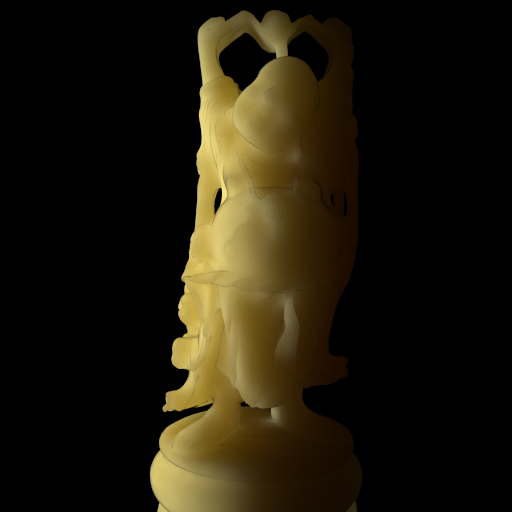
\includegraphics[width=0.5 \linewidth]{images/gamma_potato_buddha_dipole.png}
}
\subfloat[Directional Dipole]{
  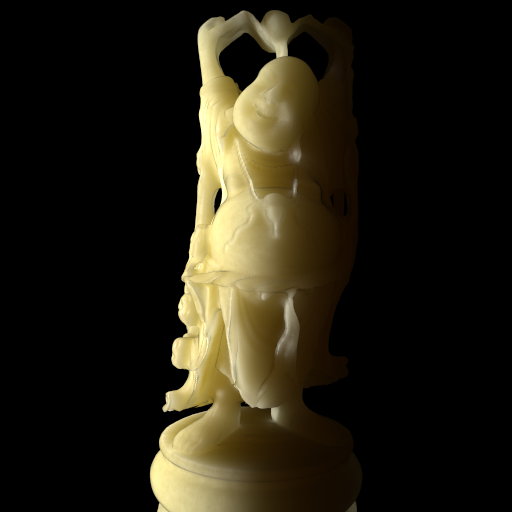
\includegraphics[width=0.5 \linewidth]{images/gamma_potato_buddha_dir.png}
}
\caption{Comparison of the standard and the directional dipole model, for a Stanford Happy Buddha made of potato, with a side directional light. We can see that  the directional dipole is able to capture finer details and provide a generally less flat appearance than the standard one.}
\label{fig:bssrdfcomparison}
\end{figure}

\chapter{Method}
In this chapter, the goal is to solve the problem that we have presented, i.e. rendering translucent materials efficiently using the directional dipole. First of all, we will start this chapter with a list of constraints and assumptions that we will use to devise our method. Secondly, we will give a theoretical justification of our method, deriving a discretization of the rendering equation that can be actually implemented in a GPU environment. Then, we will discuss some possible sampling patterns and how they could possibly improve the results of the final rendering. Then, we will introduce how the actual scattering parameters are acquired in an experimental environment, in order to obtain a plausible result. Finally, we will describe a method to approximate environment lighting using an arbitrary number of directional sources.

\section{Constraints and assumptions}

Before describing the actual method, we will introduce some constraints and assumptions on our method. Some of these assumptions and constraints are well known to the graphics community, and they are generally introduced to allow better performance, quality and flexibility. Being a real-time rendering method implies that performance plays a big part in the decisions made in the process, but since the method uses a physically based approximation the final quality of the result is also important. In the process the aspect of flexibility has been taken into account: the tradeoff between quality and performance should be tweakable with the fewest number of variables as possible. We will now list the assumptions we made in all the three described domains, quality, performance and flexibility, in order to later justify our method in the light of these assumptions. 

\subsection{Quality constraints}
\begin{enumerate}
	\item Being close as much as possible to a path traced solution. By close we mean that the root mean square of the comparison between our method and a path traced result under the same lighting conditions should not be over a certain threshold. 
	\item Being consistent with the directional dipole model for a wide range of material properties. In particular, show to perform well in the domain of quality where the directional dipole model excels (highly scattering materials).
	\item Being able to render under an arbitrary number of directional sources, point light sources and environment lighting.
\end{enumerate}

\subsection{Flexibility requirements}	
\begin{enumerate}
	\item Work with the less amount as possible of provided model data, i.e. only the position data and eventually the normals should be provided in order for the method to run. In particular, no unwrap of the mesh (UV mapping) should be necessary for the method to run. In case normal data are missing, generate them using a standard method to give a smooth appearance.
	\item Be possible to be integrated in a game engine environment, using data from other computations (e.g. vertices and normals from shadow mapping) and being adaptable to different lighting paths (forward and deferred shading).
  \item The quality versus performance tradeoff should be set by a potential artist or developer, with the fewest number of parameters as possible.
\end{enumerate}

\subsection{Performance requirements}

\begin{enumerate}
	\item Being real-time on a high-end modern GPU, i.e. one frame should take less that 100 ms (10 FPS) to render. The ideal result would be to reach a rendering time of less than 16 ms (60 FPS)
	\item Being as less dependent as possible from the geometrical complexity of the model.
	\item Being as less as dependent from the viewport resolution.
	\item If the desired quality is not reachable within one frame, converge towards a result in a reasonable amount of time. Techniques should be used to approximate the required quality for the intermediate result. 
	\item Maintain a reasonable performance under changing light conditions, deformations and change of parameters, with little or none performance penalties.
	\item Employ the advantages of the directional dipole model to improve performance.
	\item Support a certain number of directional and point lights (up to 3 to 5 pixel lights, as in commercial engines\citep{unitymanual}).
	\item Require little or no pre-processing in order to be able to perform. In particular, pre-processing, if any, should be general and performed only at the beginning of the life cycle of the program. 
	\item Employ and explore the latest features in the available graphics drivers and libraries. The details on which feature will be used are left to the implementation section.
\end{enumerate}

\section{Method overview}

First of all, we recall the general form of the rendering equation for participating media using a BSSRDF (equation \ref{eq:bssrdfeq}):

\begin{equation*}
L_o(\x_o,\vomega_o) = L_e(\x_i,\vomega_i) + \int_A \int_{2\pi} S(\x_i, \vomega_i, \x_o, \vomega_o) L_i(\x_i,\vomega_i) V(\x_i) (\vec{n}_i \cdot \vomega_i) d\vomega_i d A_i
\end{equation*}

In the usual approach to offline path traced rendered, for each pixel of the final image we need to integrate the radiance from all the possible sources along the path traced from the pixel in the scene. For each surface element in one pixel, all the incoming contributions from the other points in the scene must be accounted, an then multiplied by the BSSRDF function in the direction of the camera. In a way, we are basically performing the integral in \ref{eq:bssrdfeq}numerically. If we use a BSSRDF function, the contribution from all the points from the other surfaces must be employed, while in the case of a BRDF some contribution may be excluded (e.g., if there is a opaque surface between two points). Given its natural exponential explosion, path tracing is not obviously suitable for real-time rendering.

Our method, in its final goal to be real time, performs the same integral as equation \ref{eq:bssrdfeq} , but under some assumptions and restrictions that allow us to perform it more efficiently. In addition, since our method involves more how to approximate the \emph{integral} and not the BSSRDF, it is applicable to any BSSRDF function, given that it has limited or no dependence on the outgoing direction $\vomega_o$, like the directional dipole model.

The idea on approximating the integral comes from the fact that the directional dipole (and subsurface scattering effects) generally decay exponentially from the point of incidence, as we can see from figure TODO; where we show the simulation of a laser light hitting a surface in one point. So, the subsurface scattering contribution for points that are far apart becomes quickly negligible. The distance on which these effects become negligible is usually related to the transmission coefficient $\sigma_{tr}$. We will investigate this relation better in the result section. 

\begin{figure}
\centering
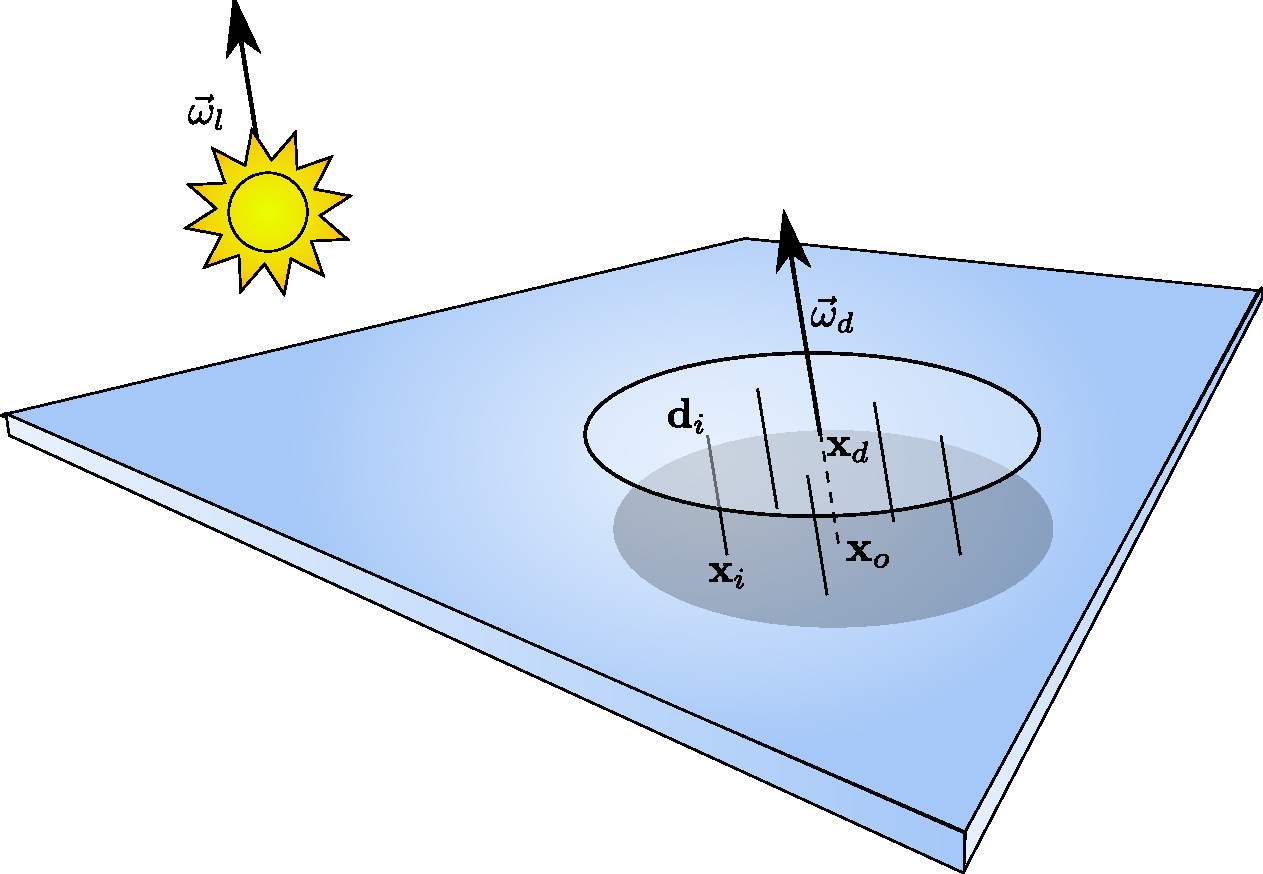
\includegraphics[width=0.8\textwidth]{images/disk_setup.pdf}
\caption{Setup for our method: the disk is placed on the point $\x_o$, displaced along the disc direction $\vomega_d$ and then the sample points $\mathbf{d}_i$ are reprojected back to find the samples $\x_i$.}
\label{fig:disksetup}
\end{figure}
\FloatBarrier

So, given this exponential decay, we place a sample disc on the surface for a position $\mathbf{x}_o$. We define a sampling disc as a point $\x_d$, a radius $r_d$ and a direction $\vomega_d$ From this disc, we chose a subset of surface points, called \emph{sample points}. To get these points, we project the points from the disc $\mathbf{d}_i$ on the surface $M$, using the disc normals as a direction (see figure \ref{fig:disksetup} for an illustration of the process). In formulas, we do:

\begin{equation*}
\x_i = \mathbf{d}_i - s \vomega_d, s \in \mathbb{R}, \x_i \in M
\end{equation*}

Then, we calculate and average the BSSRDF contribution from these points $\x_i^k$ on the point $x_o$. The process can be repeated more times for multiple lights, using the same sampling points. 

Given this set up, we need to find a way of efficiently placing the disc in order to get a good approximation of the BSSRDF. In fact, if the disc is placed in the wrong position, the accounted contribution from the sampling points will not be correct. Moreover, also the orientation of the disc is important, in order to not undersample light in certain regions of the model. . A na\"{i}ve approach would suggest to pick $\x_d = \x_o$ and $\vomega_d = \vec{n}_o$, but we can see that this approach is not correct. The most obvious counter examples are displayed in Figure \ref{fig:discwrong}: in the first example \ref{fig:discwrongpoint}, the contribution from the surrounding points will be zero, because none of the sampling points is directly illuminated by the light, so the visibility term on the rendering equation will evaluate to zero. In the second example (figure \ref{fig:discwrongdir}), the wrong direction $\vec{n}_o$ prevents the most of the points from being sampled.

\begin{figure}
\centering
\subfloat[Bottom sample, na\"{i}ve approach]{
  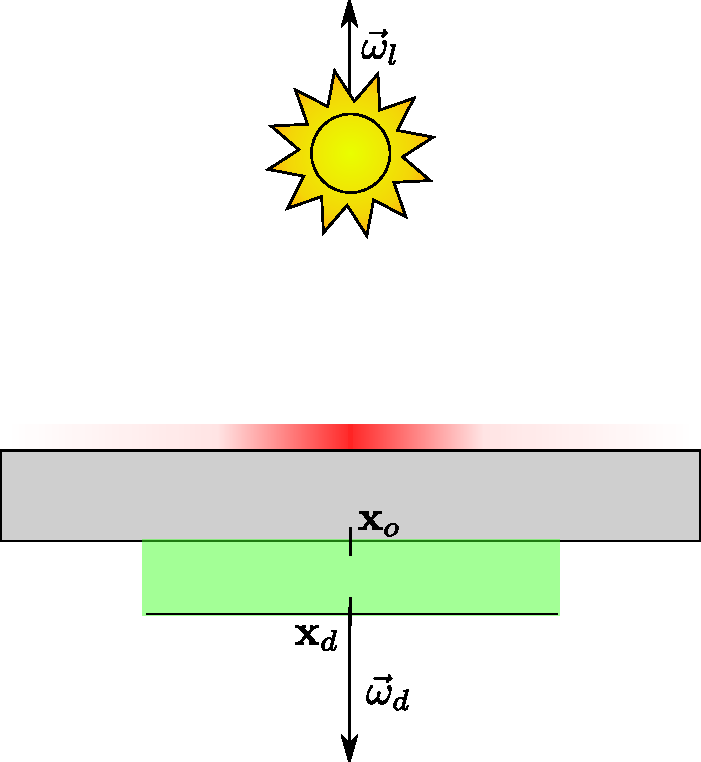
\includegraphics[width=0.5 \linewidth]{images/distribution_wrong_1.pdf}
  \label{fig:discwrongpoint}
}
\subfloat[Side sample, na\"{i}ve approach]{
  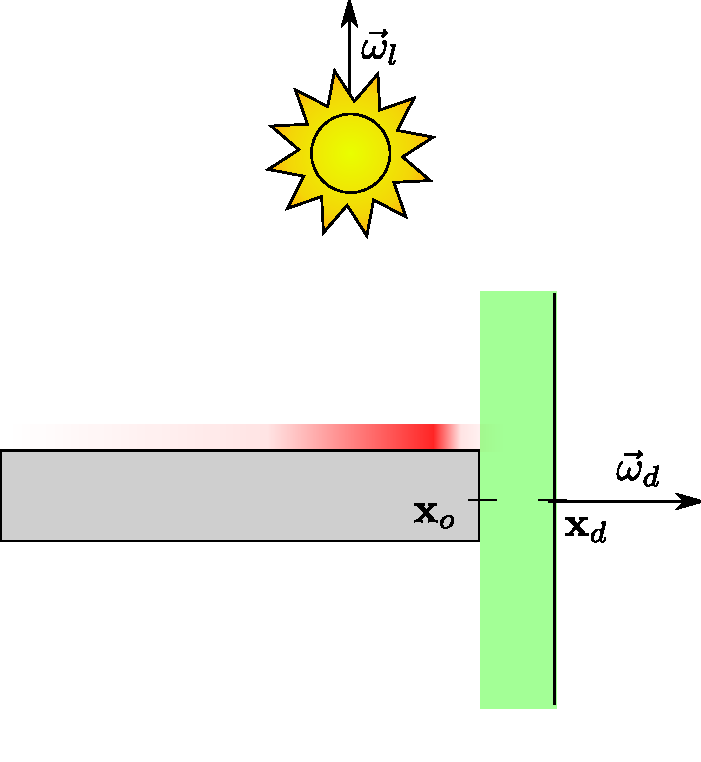
\includegraphics[width=0.5 \linewidth]{images/distribution_wrong_3.pdf}
  \label{fig:discwrongdir}
} 
\caption{Counter examples of the na\"{i}ve choice for $\x_d$ and $\vomega_d$. The green area represent the sampling area of the disc (see from the side). The red area shows where on the surface the contribution is higher for the point $\x_o$. We can see that with this approach all the contribution is actually missed.}
\label{fig:discwrong}
\end{figure}

A more careful choice for placing the points in the disc is to place the disc in a way that the obtained surface point is always the closest one to the light. To ensure that the points $\x_i$ always have this property, we can place $\x_d$ far enough from the surface in a way that all the sampling points have to be the closest to the light. If we define a \emph{bounding box vector} $\mathbb{b}$ in the same coordinate frames, we have a simple formulation for $\x_d$:

$$
\x_d = \x_o + (\mathbf{b} \cdot \vomega_l) \vomega_l
$$

The bounding box vector is a vector where its components are the maximum extension of the mesh in the coordinate reference system. So,

$$
\mathbf{b} = (\max(\x_i^x) - \min(\x_i^x), \max(\x_i^y) - \min(\x_i^y), \max(\x_i^z) - \min(\x_i^z))
$$ 

To solve the problem in the second example in figure \ref{fig:discwrongdir}, we chose to always orient the circle towards the light, that is $\vomega_d = \vomega_l$ for directional lights and $\vomega = \frac{\x_l - \x_d}{\|\x_l - \x_d\|}$ for point lights. As we can see, for the new choices of disc placement and orientation we are able to catch the points from where the contribution is stronger. This new setup seems much more complicated that the na\"{i}ve approach, but as we will see in the implementation section the Z-buffer of the GPU will permit us to get the requested point without any additional computation.

\begin{figure}
\centering
\subfloat[{Bottom sample, our method}]{
  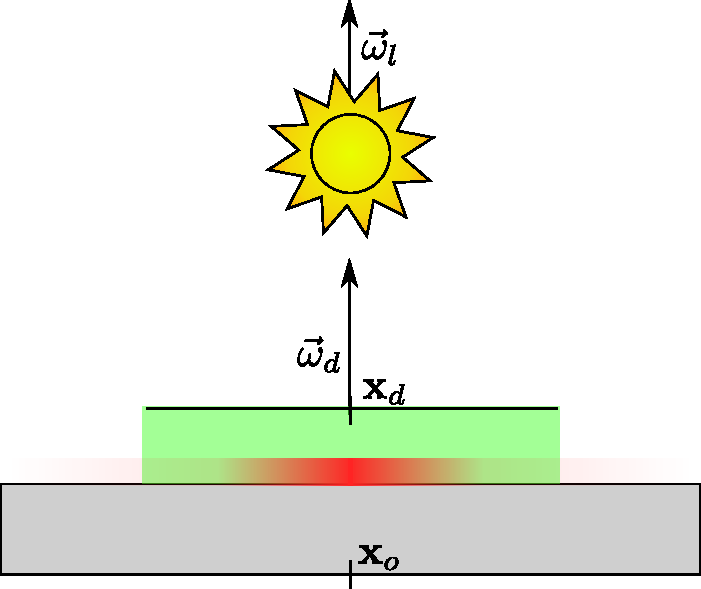
\includegraphics[width=0.5 \linewidth]{images/distribution_wrong_2.pdf}
  \label{fig:discrightpoint}
}
\subfloat[{Side sample, our method}]{
  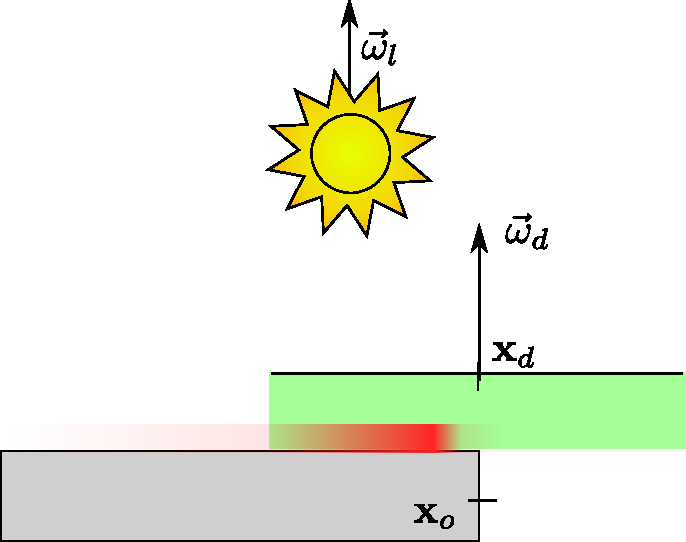
\includegraphics[width=0.5 \linewidth]{images/distribution_wrong_4.pdf}
  \label{fig:discrightdir}
} 
\label{fig:discright}
\caption{The counter examples of figure \ref{fig:discwrong} updated using our method of choice for $\x_d$. We can see that now most of the radiance distribution is accounted for.}
\end{figure}

For environment lights, we will see how to transform them in directional lights at the end of this chapter, so the setup of the equations will be the same for directional lights.

\subsection{Approximation of the rendering equation}

Going into the mathematical details the idea is to take the integral form of the rendering equation (equation \ref{eq:bssrdfeq}):

\begin{equation*}
L_o(\x_o,\vomega_o) = L_e(\x_i,\vomega_i) + \int_A \int_{2\pi} S(\x_i, \vomega_i, \x_o, \vomega_o) L_i(\x_i,\vomega_i) V(\x_i) (\vec{n}_i \cdot \vomega_i) d\vomega_i d A_i
\end{equation*}

First of all, we make the assumption of a body that is not emitting light: all the radiance from the body comes from an external source. This assumption can be trivially relaxed and implemented, but to simplify the equation in this chapter we will exclude it from the calculations. Secondly, we limit ourselves to the case of one directional light, treating the case of a point light later as an extension. The directional light direction $\vomega_l$ and radiance $L_d \ \delta(\vomega_d)$.

Under the first assumption, equation \ref{eq:bssrdfeq} becomes:

\begin{equation*}
\begin{split}
L_o^D(\x_o,\vomega_o) &= \int_A \int_{2\pi} S(\x_i, \vomega_i, \x_o, \vomega_o) L_d \ \delta(\vomega_l)\ V(\x_i) (\vec{n}_i \cdot \vomega_i) d\vomega_i d A_i \\
L_o^D(\x_o,\vomega_o) &= \int_A S(\x_i, \vomega_l, \x_o, \vomega_o) L_d  V(\x_i) (\vec{n}_i \cdot \vomega_l) d A_i 
\end{split}
\end{equation*}

In this way, we remove the internal integral. Then, in order to make a feasible calculation, we need to discretize the other integral as well. We imagine to have a set of $N$ points on the surface. We assume that each one of these points is visible from the light source (so we can get rid of the $V(\x_i)$ term). We will discuss in the implementation section how to make sure that all these points are visible. Each one of these points has an associated area $A_i$, so that we can write:

\begin{equation}
L_o^D(\x_o,\vomega_o) = L_d \sum_{i = 1}^N S(\x_i, \vomega_l, \x_o, \vomega_o) (\vec{n}_i \cdot \vomega_l) A_i 
\label{eq:inter1}
\end{equation}

Now, instead of using all the points on the surface, we consider only the points within a certain radius $r^*$ from the point $\x_o$. This is reasonable because because the dominating term in the directional dipole is $e^{-\sigma_{tr} r}$, so after a certain critical radius the contribution from the other points becomes negligible. Assuming the points are distributed uniformly on the circle, we obtain the following area for a point:

$$
A_i = \frac{A_c}{N \ (\vec{n}_i \cdot \vomega_l)}
$$

Where $A_c = \pi (r^*)^2$ is the area of the circle. And, by inserting into equation \ref{eq:inter1}, we obtain:

\begin{equation}
L_o^D(\x_o,\vomega_o) = L_d \frac{A_c}{N} \sum_{i = 1}^N S(\x_i, \vomega_l, \x_o, \vomega_o)
\label{eq:inter2}
\end{equation}

That is our final approximation for a directional light. For a point light, following the exact same steps, we reach a similar solution. We recall that a point light is defined by an intensity $I_p$ and a source point $\x_p$:

\begin{equation}
L_o^P(\x_o,\vomega_o) = I_p \frac{A_c}{N} \sum_{i = 1}^N \frac{S(\x_i, \frac{\x_p - \x_i}{\|\x_p - \x_i\|}, \x_o, \vomega_o)}{\|\x_p - \x_i\|^2}
\label{eq:inter3}
\end{equation}

And, since the radiance is linearly summable, we can combine the contribution from an arbitrary number of $P_1, P_2 ... P_p$ point sources and $D_1, D_2 ... D_d$ directional sources:

\begin{equation}
\begin{split}
&L_o(\x_o,\vomega_o) = \\
&= \sum_{k=1}^{p}L_o^{P_k}(\x_o,\vomega_o) + \sum_{k=1}^{d}L_o^{D_k}(\x_o,\vomega_o) \\
&= \frac{A_c}{N} \left[ \sum_{k=1}^{p}I_p^k \sum_{i = 1}^N \frac{S(\x_i, \frac{\x_p^k - \x_i}{\|\x_p^k - \x_i\|}, \x_o, \vomega_o)}{\|\x_p^k - \x_i\|^2} + \sum_{k=1}^{d} L_d^k \sum_{i = 1}^N S(\x_i, \vomega^k_l, \x_o, \vomega_o) \right] 
\end{split}
\end{equation}


\section{Sampling patterns}
As we discussed in the previous section, the BSSRDF function for the directional dipole is dominated by an exponential decay. So, it is more probable to find points that contribute more to the BSSRDF if we take points closer to the evaluation point $\x_o$. However, our assumption of uniform areas does not hold anymore, so we need to modify the previous equations in order to account for the non-linear sampling.

Assuming to have number generator that can generate numbers on a disc, we can create an exponentially distributed disc by rejection sampling. The probability distribution is:

$$
pdf(x) = \sigma_{tr} e^{-\sigma_{tr} x}
$$

We will give more detail on the process later. The radius of the point $\x_i$ is 

$$
r_i = \|\x_o^{proj} - \x_i^{proj}\|
$$

Where the two points have been projected on the circle. See figure X for more details. So now we have a new normalization term to include in order to scale back the result. So, we need now to divide by $exp(-\sigma_{tr} r_i)$ each sample. The new equation for a directional light then becomes:

$$
\hat{L}_o^D(\x_o,\vomega_o) = L_d \frac{A_c}{N} \sum_{i = 1}^N S(\x_i, \vomega_l, \x_o, \vomega_o) e^{-\sigma_{tr} r_i}
$$

The other two equations TODO and TODO change accordingly:

$$
\hat{L}_o^P(\x_o,\vomega_o) = I_p \frac{A_c}{N} \sum_{i = 1}^N \frac{S(\x_i, \frac{\x_p - \x_i}{\|\x_p - \x_i\|}, \x_o, \vomega_o)}{\|\x_p - \x_i\|^2}  e^{-\sigma_{tr} r_i}
$$

\begin{equation}
\begin{split}
&\hat{L}_o(\x_o,\vomega_o) = \\
&= \sum_{k=1}^{p}L_o^{P_k}(\x_o,\vomega_o) + \sum_{k=1}^{d}L_o^{D_k}(\x_o,\vomega_o) \\
&= \frac{A_c}{N} \left[ \sum_{k=1}^{p}I_p^k \sum_{i = 1}^N \frac{S(\x_i, \frac{\x_p^k - \x_i}{\|\x_p^k - \x_i\|}, \x_o, \vomega_o)}{\|\x_p^k - \x_i\|^2} e^{-\sigma_{tr} r_i} + \sum_{k=1}^{d} L_d^k \sum_{i = 1}^N S(\x_i, \vomega^k_l, \x_o, \vomega_o) e^{-\sigma_{tr} r_i}\right] 
\end{split}
\end{equation}

\section{Parameter acquisition}
When rendering translucent materials, it is important that we have the right scattering properties, in order to match the appearance of real world objects. The scattering parameters may be tweaked by the artist and set up manually, but this is a long process since the the scattering properties are not directly related to material appearance. In order to avoid this problems, the scattering parameters are measured from samples taken from real world objects. In this section, we will give an overview of two methods used to estimate the scattering parameters.

The first method was presented alongside the standard dipole model by \cite{Jensen:2001:PMS:383259.383319}. The measurement apparatus consists of a series of lenses that focus the light on the sample. The light power $\Phi$ is measured by calibrating the sensor with a spectralon sample. A picture of the sample is then acquired at different exposure, in order to build an high dynamic range image. This is necessary since the scattering decays exponentially, so a high range is needed to have meaningful measurements. The measured data are then fitted to diffusion theory in order to obtain the scattering coefficients. Due to the nature of the measurement, it is not possible to measure the mean cosine $g$ of the material, but only the reduced scattering coefficient $\sigma_s' = \sigma_s (1 - g)$ and the absorption coefficient $\sigma_a$. This measurement model uses the diffusion approximation to work, so it shares the same limitations: it is valid only for materials where $\sigma_a \ll \sigma_s$.

The second method, proposed by \cite{Narasimhan:2006:ASP:1141911.1141986} proposes a method to measure the scattering coefficient by dilution. The assumption is that water does not interfere with the scattering properties of the materials dissolved within it for small distances (less than \SI{50}{cm}). Naturally, the material needs then to be already in  a liquid form, or to be a powder that can be easily dissolved in water. The setup of the experiment is a box full of water with a camera and an area light. High dynamic range picture of the material dissolved in water are then taken, and the scattering coefficients can be measured with a low error. Various measurements at different concentrations are needed in order to get an effective measurement of the coefficients, but then the coefficients can be extrapolated for any concentration. 

Some of the scattering properties measured thanks to this method are reported in table \ref{table:scatteringcoefficients}. This coefficients will be used throughout the report when referencing to a specific material.
\clearpage
\begin{landscape}
\renewcommand{\arraystretch}{1.8}
\begin{table}[!ht]
    \centering
    \begin{tabular}{|l|ccc|ccc|ccc|c|c|}
    \hline
    \multirow{2}{*}{Material}               & \multicolumn{3}{|c|}{Absorption, $\sigma_a$}     & \multicolumn{3}{|c|}{Scattering, $\sigma_s$}     & \multicolumn{3}{|c|}{Mean cosine, $g$}    & \multirow{2}{*}{$\eta$} & \multirow{2}{*}{Source} \\ 
               &R& G      & B     & R & G      & B      & R   & G     & B     &  &  \\ \hline
    {Apple}                  & 0.0030 & 0.0034 & 0.0046 & 2.29   & 2.39   & 1.97   & -     & -     & -     & 1.3    & J      \\
    {Ketchup}                & 0.061  & 0.97   & 1.45   & 0.18   & 0.07   & 0.03   & -     & -     & -     & 1.3    & J      \\
    {Marble}                 & 0.0021 & 0.0041 & 0.0071 & 2.19   & 2.62   & 3.00   & -     & -     & -     & 1.5    & J      \\
    {Potato}                 & 0.0024 & 0.0090 & 0.12   & 0.68   & 0.70   & 0.55   & -     & -     & -     & 1.3    & J      \\
    {Whole milk}             & 0.0011 & 0.0024 & 0.014  & 2.55   & 3.21   & 3.77   & -     & -     & -     & 1.3    & J      \\
    {Coffee}                 & 0.1669 & 0.2287 & 0.3078 & 0.2707 & 0.2828 & 0.297  & 0.907 & 0.896 & 0.88  & 1.3    & N    \\
    {Soy milk}               & 0.0001 & 0.0005 & 0.0034 & 0.2433 & 0.2714 & 0.4563 & 0.873 & 0.858 & 0.832 & 1.3    & N      \\
    {Wine (merlot)   }       & 0.7586 & 1.6429 & 1.9196 & 0.0053 & 0      & 0      & 0.974 & 0     & 0     & 1.3    & N      \\
    {Beer (Budweiser)}       & 0.1449 & 0.3141 & 0.7286 & 0.0037 & 0.0069 & 0.0074 & 0.917 & 0.956 & 0.982 & 1.3    & N      \\
    {White grapefruit juice} & 0.0096 & 0.0131 & 0.0395 & 0.3513 & 0.3669 & 0.5237 & 0.548 & 0.545 & 0.565 & 1.3    & N      \\ \hline
    \end{tabular}
		\caption{Scattering material parameters estimated using different methods. For the source field, \texttt{J} materials come from \cite{Jensen:2001:PMS:383259.383319}, while \texttt{N} materials come from \cite{Narasimhan:2006:ASP:1141911.1141986}. Note that the materials measured with the technique proposed in \cite{Jensen:2001:PMS:383259.383319} are without the $g$ coefficient.}
		\label{table:scatteringcoefficients}
\end{table}
\end{landscape}
\clearpage

\section{Environment lights}
\FloatBarrier

Environment lighting is a omni-directional lighting that represents lighting coming from an environment. Instead of defining a light as a direction or a point in space, we define directly the radiance distribution on a map. The map is usually provided in a hdr format in order to cover various range of radiance, and it is usually given as a set of six cube faces (cubemap) or as a latitude-longitude map, as the one in figure \ref{fig:doge}. The maps are usually given in equirectangular projection.

In the game development community, spherical harmonics (SH) \citep{green,peterpikeconference} are usually employed. This technique, given an heavy pre-computation step, transforms the radiance map into a set of coefficients in the spherical harmonics basis. This coefficients that then can be used easily to represent the radiance map, if we are interested only in the low-frequency part of it. 


\begin{figure}
\centering
\includegraphics[width=\textwidth]{images/matlab/doge2.png}
\caption{Latitude - longitude environment map of the inner courtyard of the Doge's palace in Venice. The map has been converted to a RGB format from the original HDR format. Image courtesy of \url{http://gl.ict.usc.edu/Data/HighResProbes/}.}
\label{fig:doge}
\end{figure}


In this chapter, we introduce a technique presented in \cite{Pharr:2004:PBR:975275} to convert a environment map into a set of directional light sources of arbitrary size. The general idea is to generate a set of random points and them transform them according to a pre-computed probability distribution. This distribution make the random point concentrate in areas where the radiance is higher, so that it is possible to get the most representative points on the radiance map. The found points are then transformed into a spherical coordinate basis in order to get the light direction.

We start defining our image as an array of $n$ rows and $m$ columns. We need to define a function that of each pixel of the image gives us a single radiance value. Instead of using radiance, we use luminance. The ITU-R recommendation standard gives us a formula to obtain luminance from spectral radiance values:

$$
f(u,v) = 0.2126 R(u,v) + 0.7152 G(u,v) + 0.0722 B(u,v)
$$

Where $[u,v] \in [0,n)\times [0,m)$. $R$, $G$ and $B$ represent the spectral coordinates of the radiance map. We would like to define now a probability distribution function based on the $f(u,v)$ function. We can define it simply by normalizing $f$ with the integral of the function over the domain:

$$
p(u,v) = \frac{f(u,v)}{\int \int f(u,v) du dv} = \frac{f(u,v)}{\sum_u \sum_v f(u,v)}
$$

However, in order to be able to sample from the distribution $p(u,v)$, there are some things to take care about. We would like now to separate the two variables, in order to sample from two one-dimensional distribution, instead of one two-dimensional distribution. To do this, we use the conditional probability formula:

$$
p(u,v) = p_v(v|u) p_u(u)
\label{eq:conditional_prob}
$$

So that we first choose u, sample its probability $p_u(u)$ and then compute the conditional density $p_v(v|u)$ using the found value for $u$. Using the marginal formulas, the first probability is easily found:

$$
p_u(u) =\int p(u,v) dv = \frac{\sum_v f(u,v)}{\sum_u \sum_v f(u,v)}
$$

And, from equation \ref{eq:conditional_prob}, we find the conditional probability:

$$
p_v(v|u) = \frac{p(u,v)}{p_u(u)} = \frac{f(u,v)}{\sum_v f(u,v)} \sin \theta
$$

The $\sin \theta$ comes from the fact that the latitude-longitude map with a equirectangular projection is not area preserving. So, the sampling must take into account the distortion of the map, otherwise the samples will be more concentrated at the poles, rather than distributed uniformly on the sphere. TODO IMAGE OF NOT DISTRIBUTED POINTS

Now we are ready to sample the function. In order to bias our sample according to the radiance distribution, we need to calculate the cumulative distribution function (CDF) for a one-dimensional probability distribution function. The CDF is defined as:

$$
c_u(u) = \int_{-\infty}^{u} p_u(u) du = \sum_{i=0}^u p_u(u)
$$

That is the discrete integral of the function up to the point $u$. Figure \ref{fig:cdfweight} explain why. If, as the figure, all the radiance is distributed towards the right side of the picture (i.e. the CDF rises slowly), if we pick a set of random points and reverse the CDF on them, we obtain a new set of points that is biased towards the highest concentration of radiance.

%\begin{figure}
%\centering
%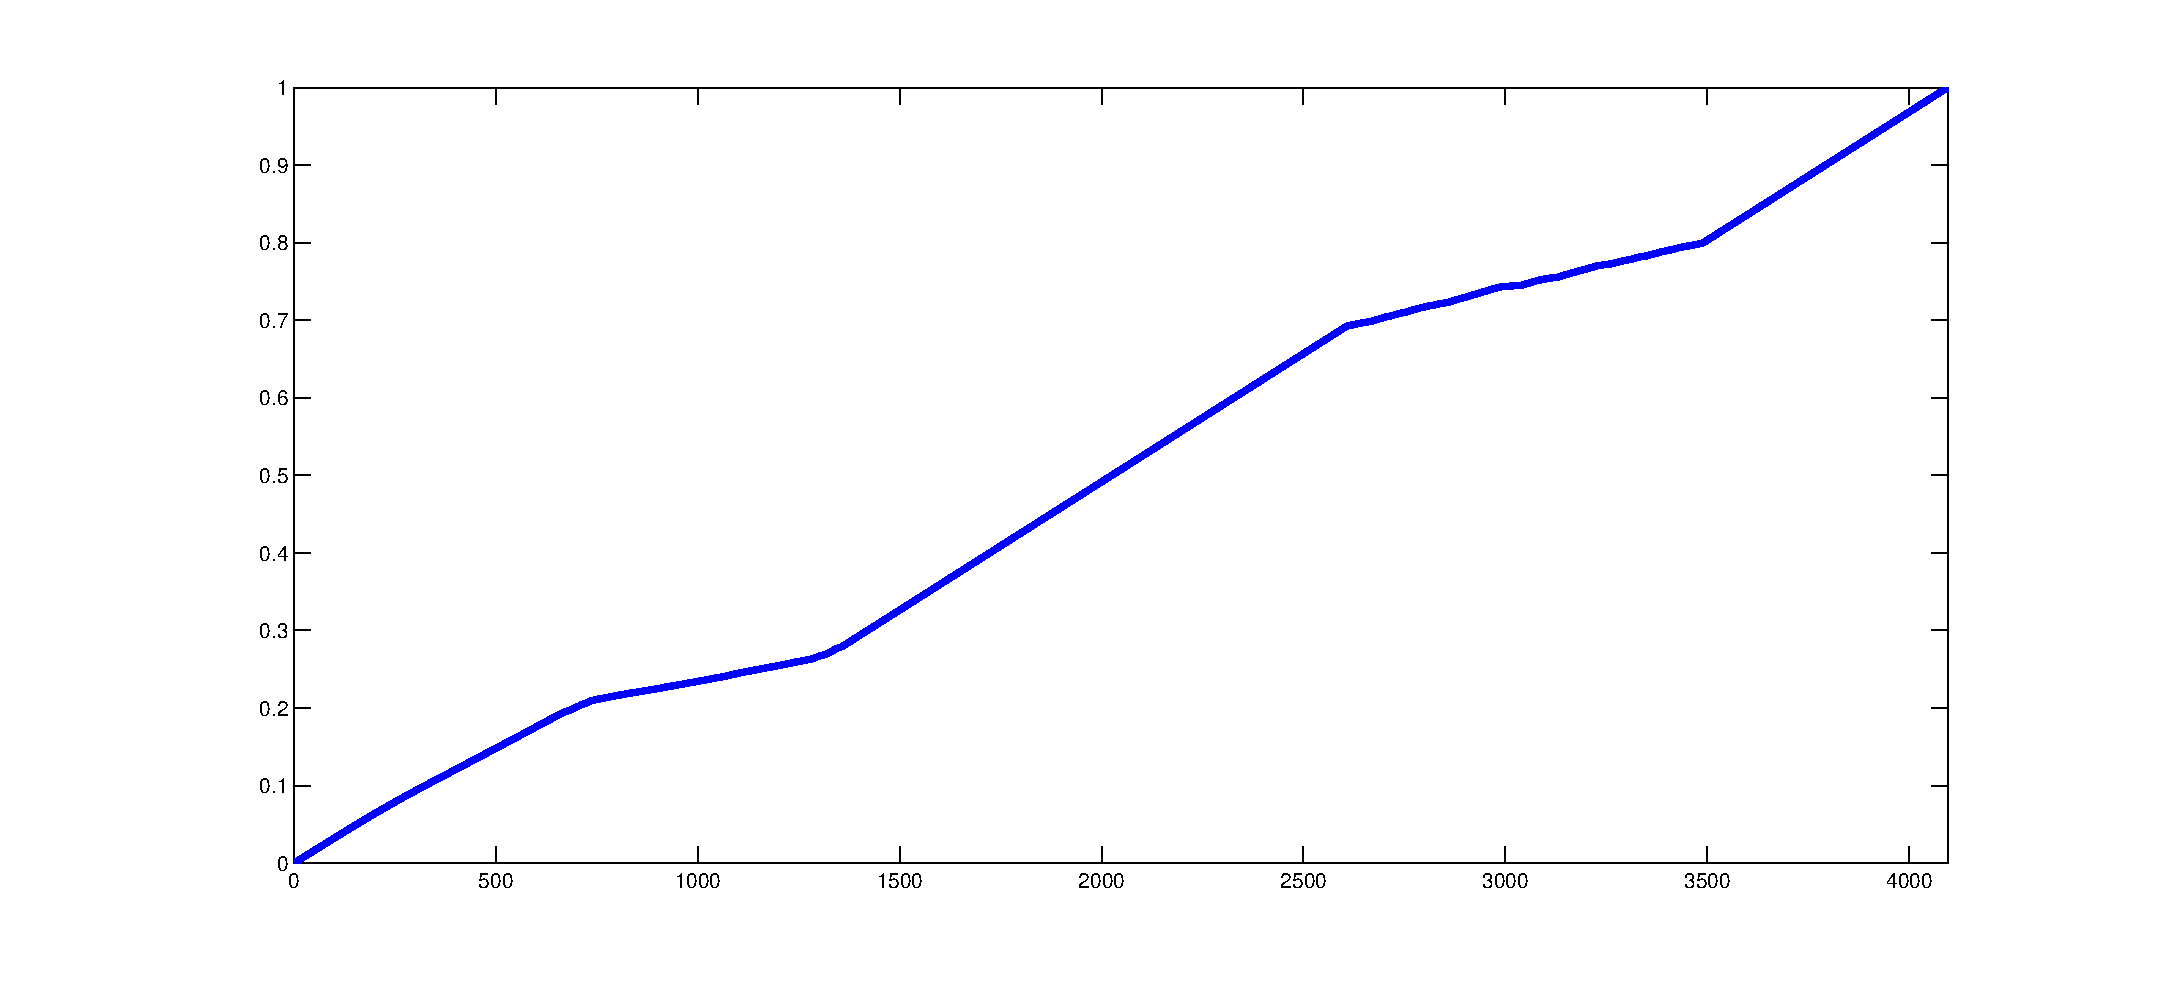
\includegraphics[width=\textwidth]{images/matlab/doge_green_line.eps}
%\caption{CDF for luminance of line 450 of the doge skybox.}
%\label{fig:cdf}
%\end{figure}

\begin{figure}
\centering
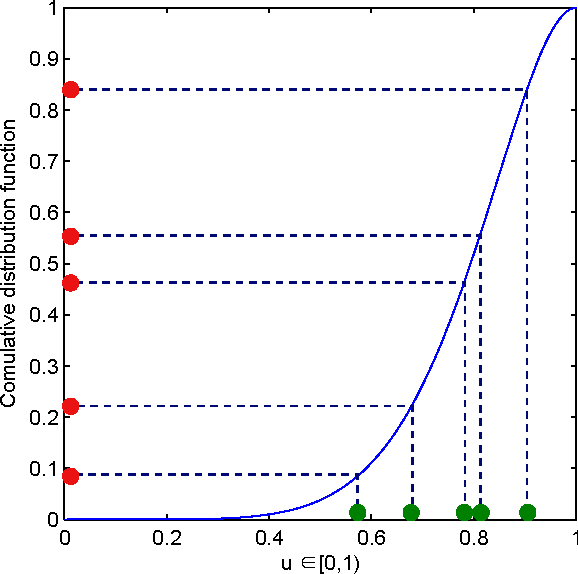
\includegraphics[width=0.7\textwidth]{images/matlab/cdfex.pdf}
\caption{Effect of weighting values with the CDF. We note that the random values on the $y$ axis are transformed and accumulated where the CDF is steeper.}
\label{fig:cdfweight}
\end{figure}

Let us now pick a couple of random points $(\zeta_1,\zeta_2) \in [0,1)^2$. We then convert these points to a pair of coordinates $(u_b,v_b) \in [0,n)\times[0,m)$ by inverse sampling of the CDF. We will give the details of how to discretize this process in the implementation section. Then, we obtain the spherical coordinates using the standard formula:

$$
(\theta, \phi) = \left(\frac{u_b}{n\pi}, \frac{v_b}{2 \pi m}\right)
$$

And, from the spherical coordinates, we use the equirectangular projection formula to transform them into a vector in the 3D space, that is the final direction for our light.

$$
\vomega_l = (\cos\phi\  \sin\theta, \sin\phi\  \sin\theta, \cos\theta)
$$

And, by varying the random values $(\zeta_1,\zeta_2)$, obtain a set of directions that we can use for rendering. The generated points for the Doge map can be seen in figure TODO.
%\chapter{Implementation}
\label{chap:implementation}
In this chapter, we will introduce the implementation of our method. In this chapter we will focus on a GPU-oriented implementation of the method presented in chapter \ref{chap:method}. First, we will briefly introduce the environment in which we are operating. Then, we will give a general outline of our algorithm. Then, we will discuss in more detail some of the ideas introduced in the algorithm overview. After this discussion, we will discuss some defects and artifacts in our algorithm that arose during the implementation, and how we have solved them. Finally, we will extend our implementation to different kind of lights. Finally, we will discuss our implementation, introducing some possible implementation alternatives.

\section{Environment}

In order to better contextualize some of the choices and the code parts that will be introduced in this section, we will first introduce the environment used in our implementation. The method we are going to discuss was made using the OpenGL API, version 4.3 (released in August 2012), a multi-platform API used for rendering 2D and 3D accelerated graphics. With the OpenGL API comes GLSL, the \emph{OpenGL Shading Language}, used for writing pieces of code to be run on the GPU, called \emph{shaders}. Our method uses some advanced features of OpenGL 4.3, so it is not immediately portable to previous generation hardware, and runs only on high-end modern GPUs. On the CPU side, we use an extended framework based on Qt, a C++ library that allows to create OpenGL contexts and graphical interfaces in an easy way.

\section{Algorithm overview}

By keeping the limitations presented in chapter \ref{chap:intro} in mind and introduced in \ref{sec:quality}, we introduce our algorithm. The algorithm is inspired by \emph{translucent shadow maps} \citep{Dachsbacher:2003:TSM:882404.882433}, that we presented in chapter \ref{chap:previous}. The general idea is to first render the scene from the light point of view, then place the disk we discussed in the previous chapter (section \ref{sec:m_overv}) directly on the generated texture, storing the result in a radiance map. We use many directions in order to capture all the sides of the object. Finally, we sample from the radiance map for the final rendering.

In this section, we will assume to only have one directional light $L_d$, $\vomega_d$ and one not-deformable object in the scene. We will discuss later how to extend the method to multiple light sources.

\textbf{Step 1 - Light buffer} \\

In the first step, positions and normals of the object are rendered into a texture from the light point of view. The resulting texture is called the \emph{light map}. As in standard shadow mapping we create and store a matrix to convert between world space and texture light space. Depth testing in this step is enabled. More details on the implementation of a render to texture are presented in section \ref{sec:rendertotexture}.

\begin{figure}[!ht]
\centering
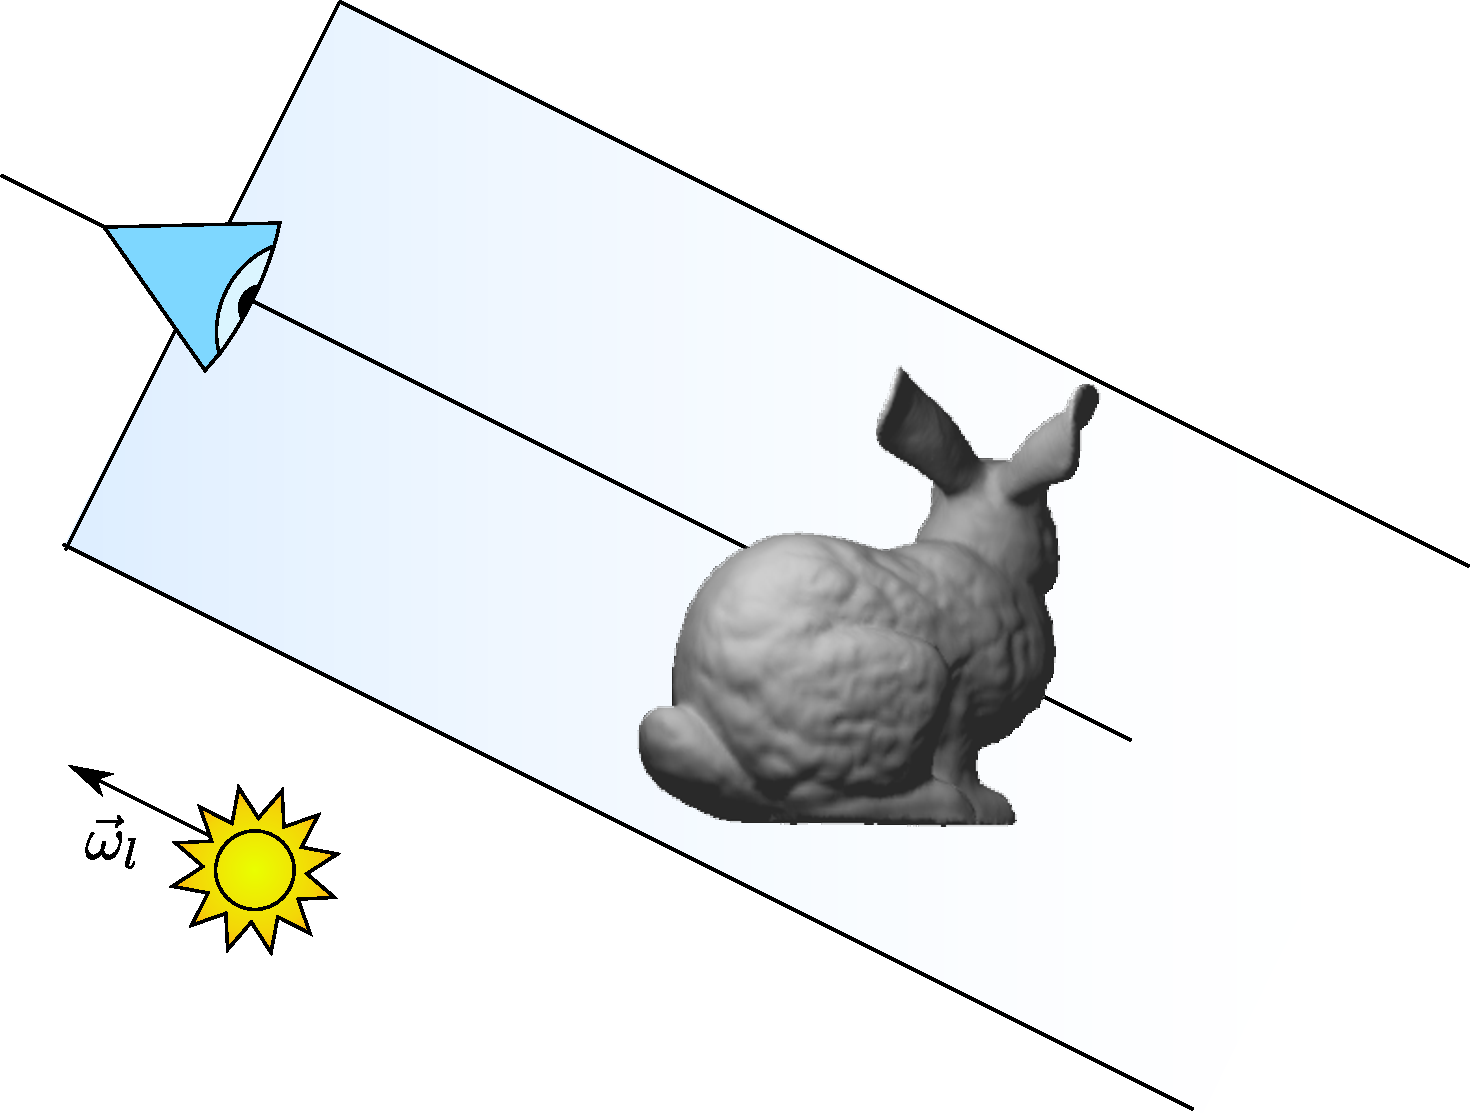
\includegraphics[width=0.8 \linewidth]{images/method/step1.pdf}
\caption{Render to G-buffer. Note that the frustum and the light direction are aligned.}
\label{fig:step1}
\end{figure} 


\begin{figure}
\centering
\subfloat[{Vertex buffer}]{
  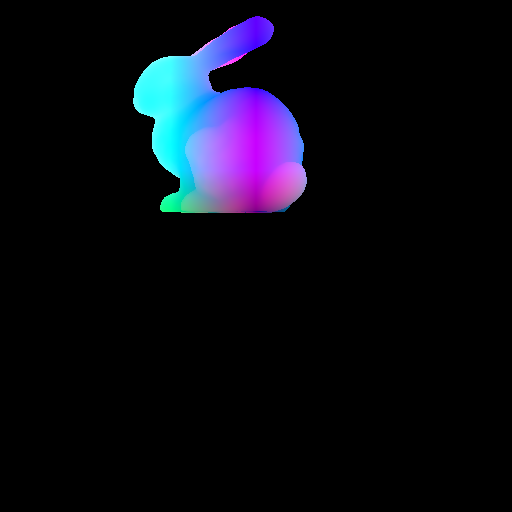
\includegraphics[width=0.5 \linewidth]{images/method/vertices.png}
  \label{fig:vbuff}
}
\subfloat[{Normal buffer}]{
  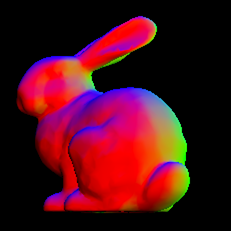
\includegraphics[width=0.5 \linewidth]{images/method/normals.png}
  \label{fig:nbuff}
} 
\label{fig:lightbuffers}
\caption{State of the vertex and normal buffer after rendering from a directional light. The model used was the Stanford bunny from the Standford 3D Scanning repository.}
\end{figure}

\textbf{Step 2 - Render to radiance map} \\
In the second step, we render the object from $K$ different directions into another texture, called the \emph{radiance map}. The radiance map is organized as a layered texture, where each layer represents a direction. More details on render to texture and layered textures are presented in sections \ref{sec:rendertotexture} and \ref{sec:layeredrendering}. The points on which to place the cameras are chosen randomly, distributed on a sphere (see section \ref{sec:random} for the details). 

On each layer, we accumulate the result over different frames (more details on it will be given later in this section). On the rendering step, for each pixel that corresponds to an exitance point $\x_o$ the shader samples $N$ points from the texture rendered in the previous step. If the sampled point is valid, it is then used to calculate the BSSRDF and accumulate it in the resulting radiance map. So, this step calculates the following:

$$
R^{k}(\x_o) = L_d \sum_{i = 1}^N S(\x^{k}_i, \vomega_l, \x_o, \vomega_o) \exp\left(\sigma_{tr} r^{k}_i\right), \ \ k \in [0,K-1] 
\label{eq:evolution_step}
$$

\begin{figure}[!ht]
\centering
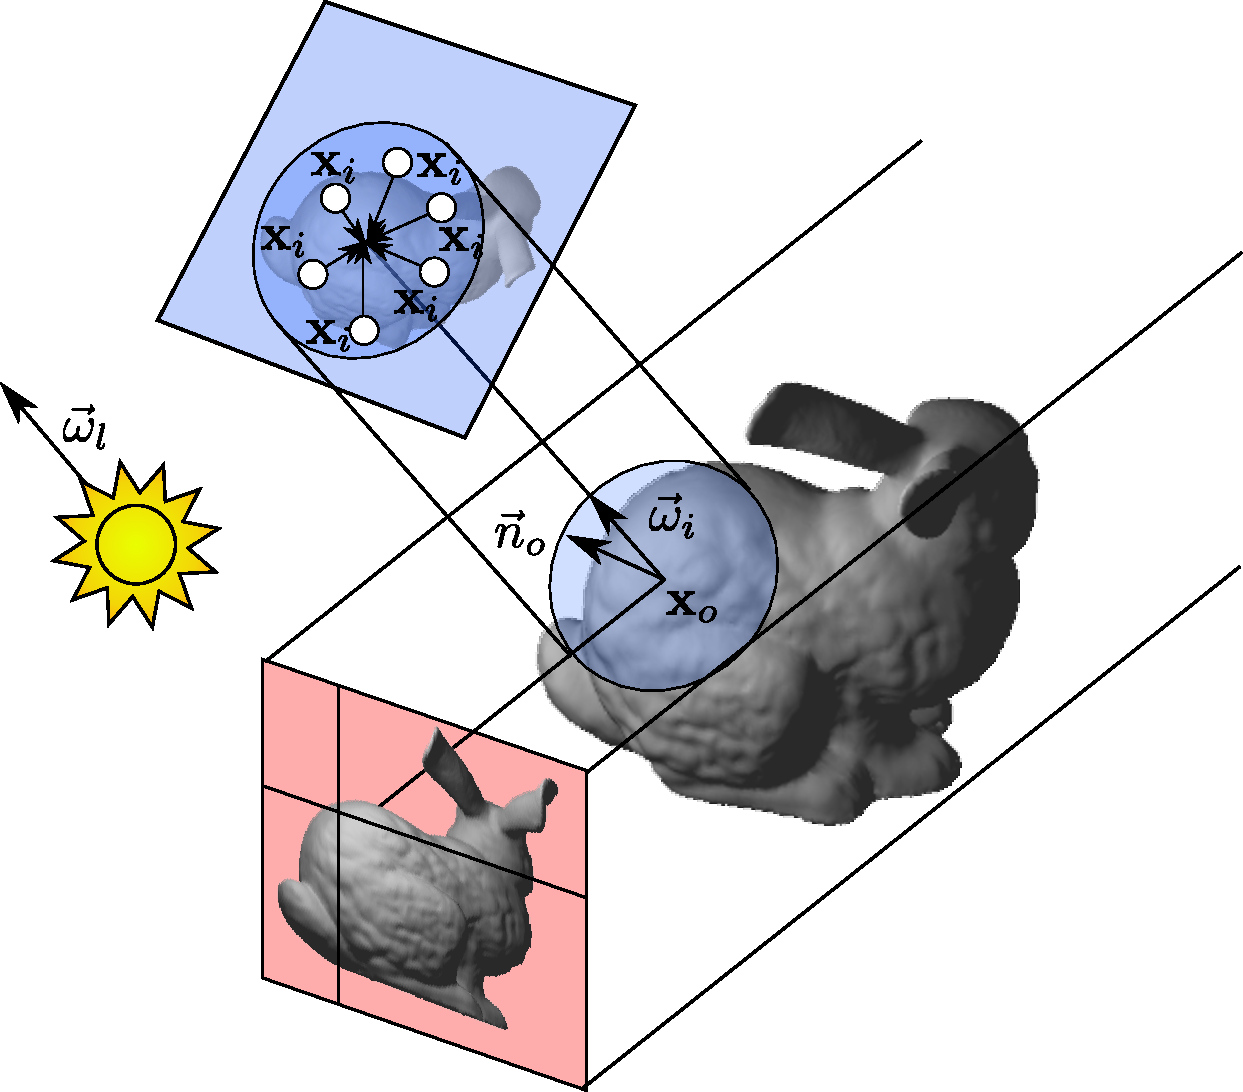
\includegraphics[width=0.9 \linewidth]{images/method/step2_improved.pdf}
\caption{Render to the radiance map. When we render the point $\x_o$, the position in the light map is calculated and the values $\x_i$ in the samples are calculated and summed over.}
\label{fig:step2}
\end{figure} 

Where we recall that we have introduced an exponential term in order to compensate for the exponential displacement of the sampling pattern (the generation of the samping pattern is described in section \ref{sec:exponentiallybiased}). We introduced a $k$ parameter, that represents the current direction we are rendering to. We can see how we are rendering a point from one of the considered directions in Figure \ref{fig:stepfrustum}. Also in this case, the texture space - world space conversion matrices are stored and prepared to be reused in the final combination step. 

We can appreciate that rendering the light from the camera point of view comes with two important advantages:

\begin{itemize}
	\item If the disk is placed in texture space, it is automatically oriented towards the light direction, that is $\vomega_d = \vomega_l$.
	\item The light renders in the texture only the points directly visible from it, that are also the only points directly lit. In addition, if we sample the light map on any point, we get the corresponding vertex that is closest to the light.
\end{itemize}

This two factors allows us to sample the most optimal point and direction in where to place the disk, as we described it in section \ref{sec:m_overv}.
 
\begin{figure}[!ht]
\centering
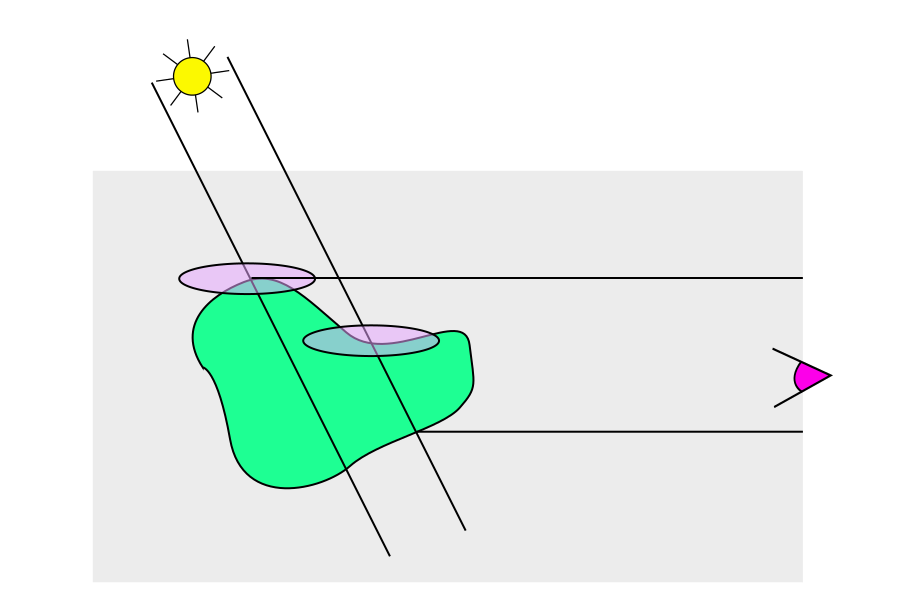
\includegraphics[width=\linewidth]{images/method/step2}
\caption{Render to cubemap, side view. The gray area represents the frustum of the current direction's camera (orthographic). We have three different cases of a point on the surface: $\x_o^1$ is visible from both the light and the camera, so the disk is placed on it. $\x_o^2$ is visible from the camera but not from the light, so the disk is placed in the closest position to the light. $\x_o^3$ is not visible from the camera, so it is discarded.}
\label{fig:stepfrustum}
\end{figure} 

In addition to this, there is an accumulation process going on:

$$
\tilde{R}^{t,k} = \sum_{i = 0}^{t-1} R^{i,k} + R^{t,k} = \tilde{R}^{t-1, k} + R^{t,k}
$$

$\tilde{R}$ here represents the value that is stored in the radiance map. In equation \ref{eq:evolution_step}, we omitted the dependence from time for the sake of clarity. We need an accumulation process in order to deal with the fact that the result from the previous computation are not reaching a satisfying result within one frame, so they need to be accumulated over a period of $T$ frames in order to reach an appreciable result. In order to do this, the sampled points need to change on different frames (in section \ref{sec:random} we give more details on the process). 

Naturally, the accumulation process works only if the scene does not change. A change can be a relative change of positions between the points on the model and the light, so if the model gets rotated or scaled (translation for directional lights is irrelevant), the accumulated result has to be discarded and the accumulation started all over. The cameras are locked with the model, so the pixels are always aligned. This is why in equation \ref{eq:evolution_step} the dependence from time of the point $\x_o$ and $\vomega_o$ have been dropped. 
 
\textbf{Step 3 - Combination} \\
In this step, we have the final render of our model. Using the matrices and the textures prepared in the previous step, for each fragment on the surface we sample all the layers in the texture as illustrated in Figure \ref{fig:step3}. In order to do this, we need also to sample the depth map generated in the previous step. We can define this sampling as a visibility function to test if a point $\x$ belongs to layer $k$:

$$
V^k(\x) = \begin{cases}
1 & \text{if $\x$ is visible from the $k$th camera} \\
0 & \text{otherwise}
\end{cases}
$$

The function $V$ is calculated by sampling the $kth$ layer depth map in a way similar to shadow mapping (details in section \ref{sec:shadow_map}). Given this function, we can simply represent the outgoing radiance by simply averaging the summation over the $K$ layers:

$$
L_{SS}^t(\mathbf{x}) = \frac{A_c}{N (t)} \frac{\displaystyle\sum_{k = 0}^{K-1}V^k(\x) \tilde{R}^{t,k}(\mathbf{x})}{\displaystyle\sum_{k = 0}^{K-1}V^k(\x)}
$$

The first factor $\frac{1}{t}$ is to average over the number of frames, while the second is the average area of a sample in the circle $\frac{A_c}{N}$, that is necessary to complete equation \ref{eq:inter2}. We note that we tried to move all the layer-independent computation into the final computation step, in order to save as much performance as possible. 

\begin{figure}[!ht]
\centering
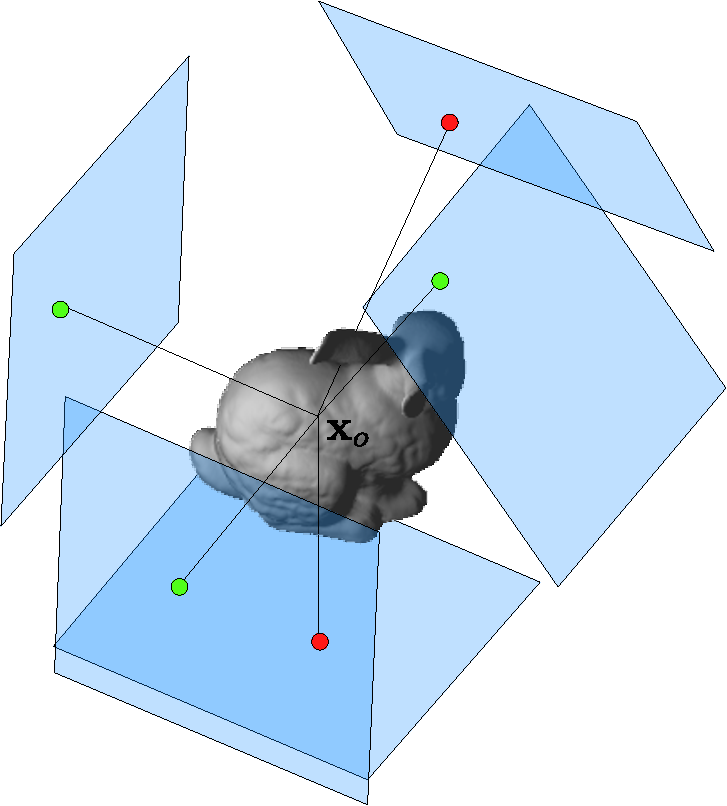
\includegraphics[width=0.6 \linewidth]{images/method/combination.pdf}
\caption{Final combination step. The blue quads indicates each one of the radiance map layers, as seen from their direction. We can see that in the point $\x_o$ the contribution from three faces (green dots) is considered. For the remaining two faces (red dots), the contribution is not considered as the point is not visible.}
\label{fig:step3}
\end{figure} 

We are not done yet, as for now we have computed the radiance only deriving from subsurface scattering. For finally describing the illumination of our scene, we need also to include a factor based on the surface reflection. Since the subsurface scattering radiance is already multiplied by a transmittance Fresnel term (in the BSSRDF equation in \ref{eq:bssrdfgen}) $T(\eta,\vomega_o)$ we the reflection color multiplied by the converse transmission term $1 - T(\eta,\vomega_o)$:

$$
L^t(\x, \vomega_o) = L_{SS}^t(\x) + (1 - T(\eta,\vomega_o)) L_i(\x, \vomega_o - 2 (\vomega_o \cdot \vec{n}) \vec{n})
$$

$L_i$ can be the radiance coming from other objects or by an environment map. After this, we just need to perform gamma correction in order to get the final result. Given the gamma coefficient $\gamma$, we perform gamma correction by:

$$
L_{gamma}^t(\x, \vomega_o, \gamma) = L^t(\x,\vomega_o)^{\frac{1}{\gamma}}
$$

And we can finally send the radiance to the output device.

\begin{figure}[!ht]
\centering
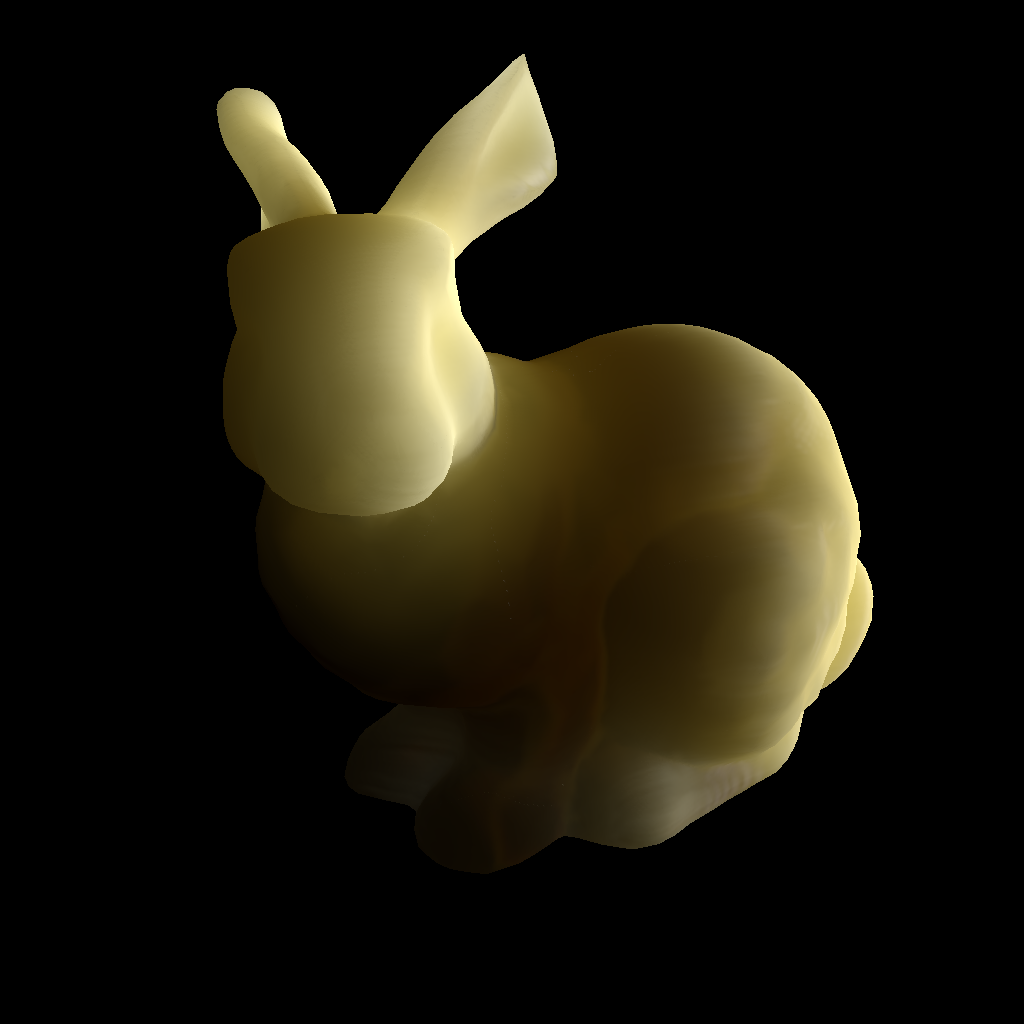
\includegraphics[width=0.8 \linewidth]{images/results/potato_100_convergence.png}
\caption{Final Result of the method after 100 frames simulating a potato bunny of dimensions $\approx 30 cm$. The parameters used were $r = 1 dm$, $N = 128$. All the results presented in this chapter are gamma corrected with $\gamma = 2.2$.}
\label{fig:potato_result}
\end{figure} 

\begin{figure}[!ht]
\centering
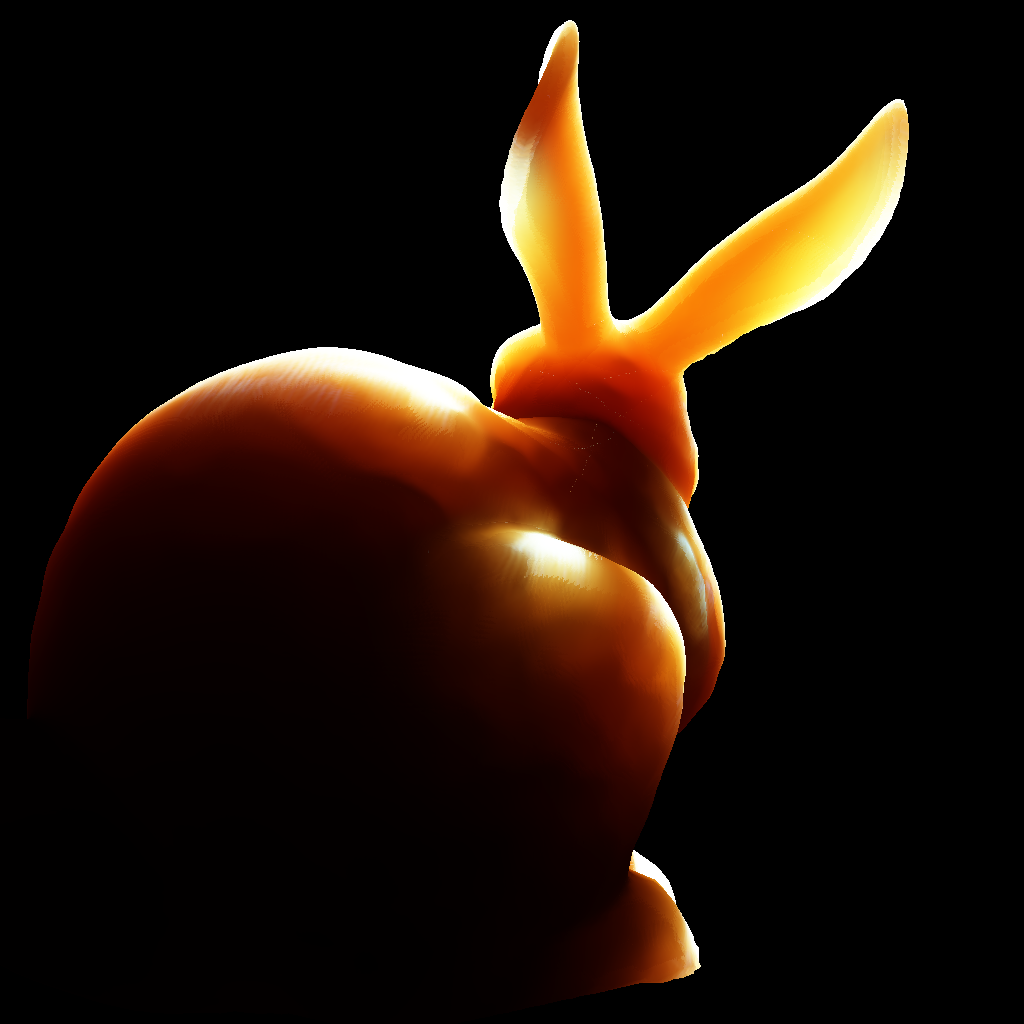
\includegraphics[width=0.8 \linewidth]{images/results/beer_backlit_100_convergence.png}
\caption{Final Result of the method after 100 frames simulating a backlit bunny made of beer, dimensions $\approx 30 cm$. The parameters used were $r = 3 dm$, $N = 128$.}
\label{fig:beer_result}
\end{figure} 
 

\section{Implementation details}
In this section, we will further expand the overview given in the previous section by adding further details. We organized this section in topics, rather than following the order given by the algorithm, since most of the topics we will introduce will be later used in multiple places. Each point clarifies with examples one technique or approach used in the method. The code given on each example does not necessarily come from our implementation, but it can be simplified for illustration purposes.

\subsection{Render-to-texture}
\label{sec:rendertotexture}
In a graphics API, and more specifically in OpenGL, all the output from a final shader stage is usually sent to the display device in order to be displayed on the screen. However, it is possible to redirect the output into another memory area of the GPU and reuse it for further computations. This allows to create complicated rendering techniques such as the ones described in this report. 

In OpenGL, is possible to redirect the output more specifically to a texture object. We can do this through a so-called \emph{framebuffer object} (FBO). A FBO is a complex collection of objects that allows off-screen rendering. A FBO has \emph{attachment points}, to which we can attach textures. A texture can be attached to one of the output color channels of the fragment shader (\gl{GL_COLOR_ATTACHMENT0}, \gl{GL_COLOR_ATTACHMENT1}, ...), to the depth buffer output (\gl{GL_DEPTH_ATTACHMENT}) or to the stencil buffer output (\gl{GL_STENCIL_ATTACHMENT}).

The connection between the framebuffer and the texture can be set in a initialization step (listing \ref{lst:rendertotextureinit}). Then, by simply binding the FBO (listing \ref{lst:rendertotexturerender}) we will redirect our screen output to the desired texture.

\begin{lstlisting}[language=C++,label=lst:rendertotextureinit,caption={Render to texture example, initilalization phase. Note the call to \gl{glFramebufferTexture2D}}]
GLuint tex,fbo;
// Generating texture
glGenTextures(1, &tex);
glBindTexture(GL_TEXTURE_2D, tex);
[...] // setting up texture parameters...
glTexImage2D(GL_TEXTURE_2D, 0, GL_RGBA16F, size, size, 0, GL_RGBA, GL_FLOAT, 0);

glGenFramebuffers(1,&fbo);

// connecting current fbo and texture
glBindFramebuffer(GL_DRAW_FRAMEBUFFER, fbo);
glFramebufferTexture2D(GL_DRAW_FRAMEBUFFER, GL_COLOR_ATTACHMENT0, GL_TEXTURE_2D, tex, 0);
glBindFramebuffer(GL_DRAW_FRAMEBUFFER, 0); //Binding back main framebuffer
\end{lstlisting}

\begin{lstlisting}[language=C++,label=lst:rendertotexturerender,caption={Render to texture example, rendering phase. Since we have not configured and FBO for depth and stencil buffers, depth testing and stencil should be disabled at this point.}]
glBindFramebuffer(GL_DRAW_FRAMEBUFFER, fbo);
GLenum buffers[] = {GL_COLOR_ATTACHMENT0};
glDrawBuffers(1, buffers);
[...] // draw model
\end{lstlisting}

\subsection{Layered rendering}
\label{sec:layeredrendering}
Layered rendering is a special feature used to render to a type of texture called \emph{layered texture}. Let us take as an example the step 2 of our algorithm, where we need to render the object from $K$ different directions. A first approach to this would be to create $K$ 2D textures of type \gl{GL_TEXTURE_2D}, and perform $K$ draw calls, rebinding the texture on the current FBO each time. OpenGL, however, provides a way to do this faster, and with a single draw call, potentially reducing the rendering costs due to context switching.

\begin{figure}[!ht]
\centering
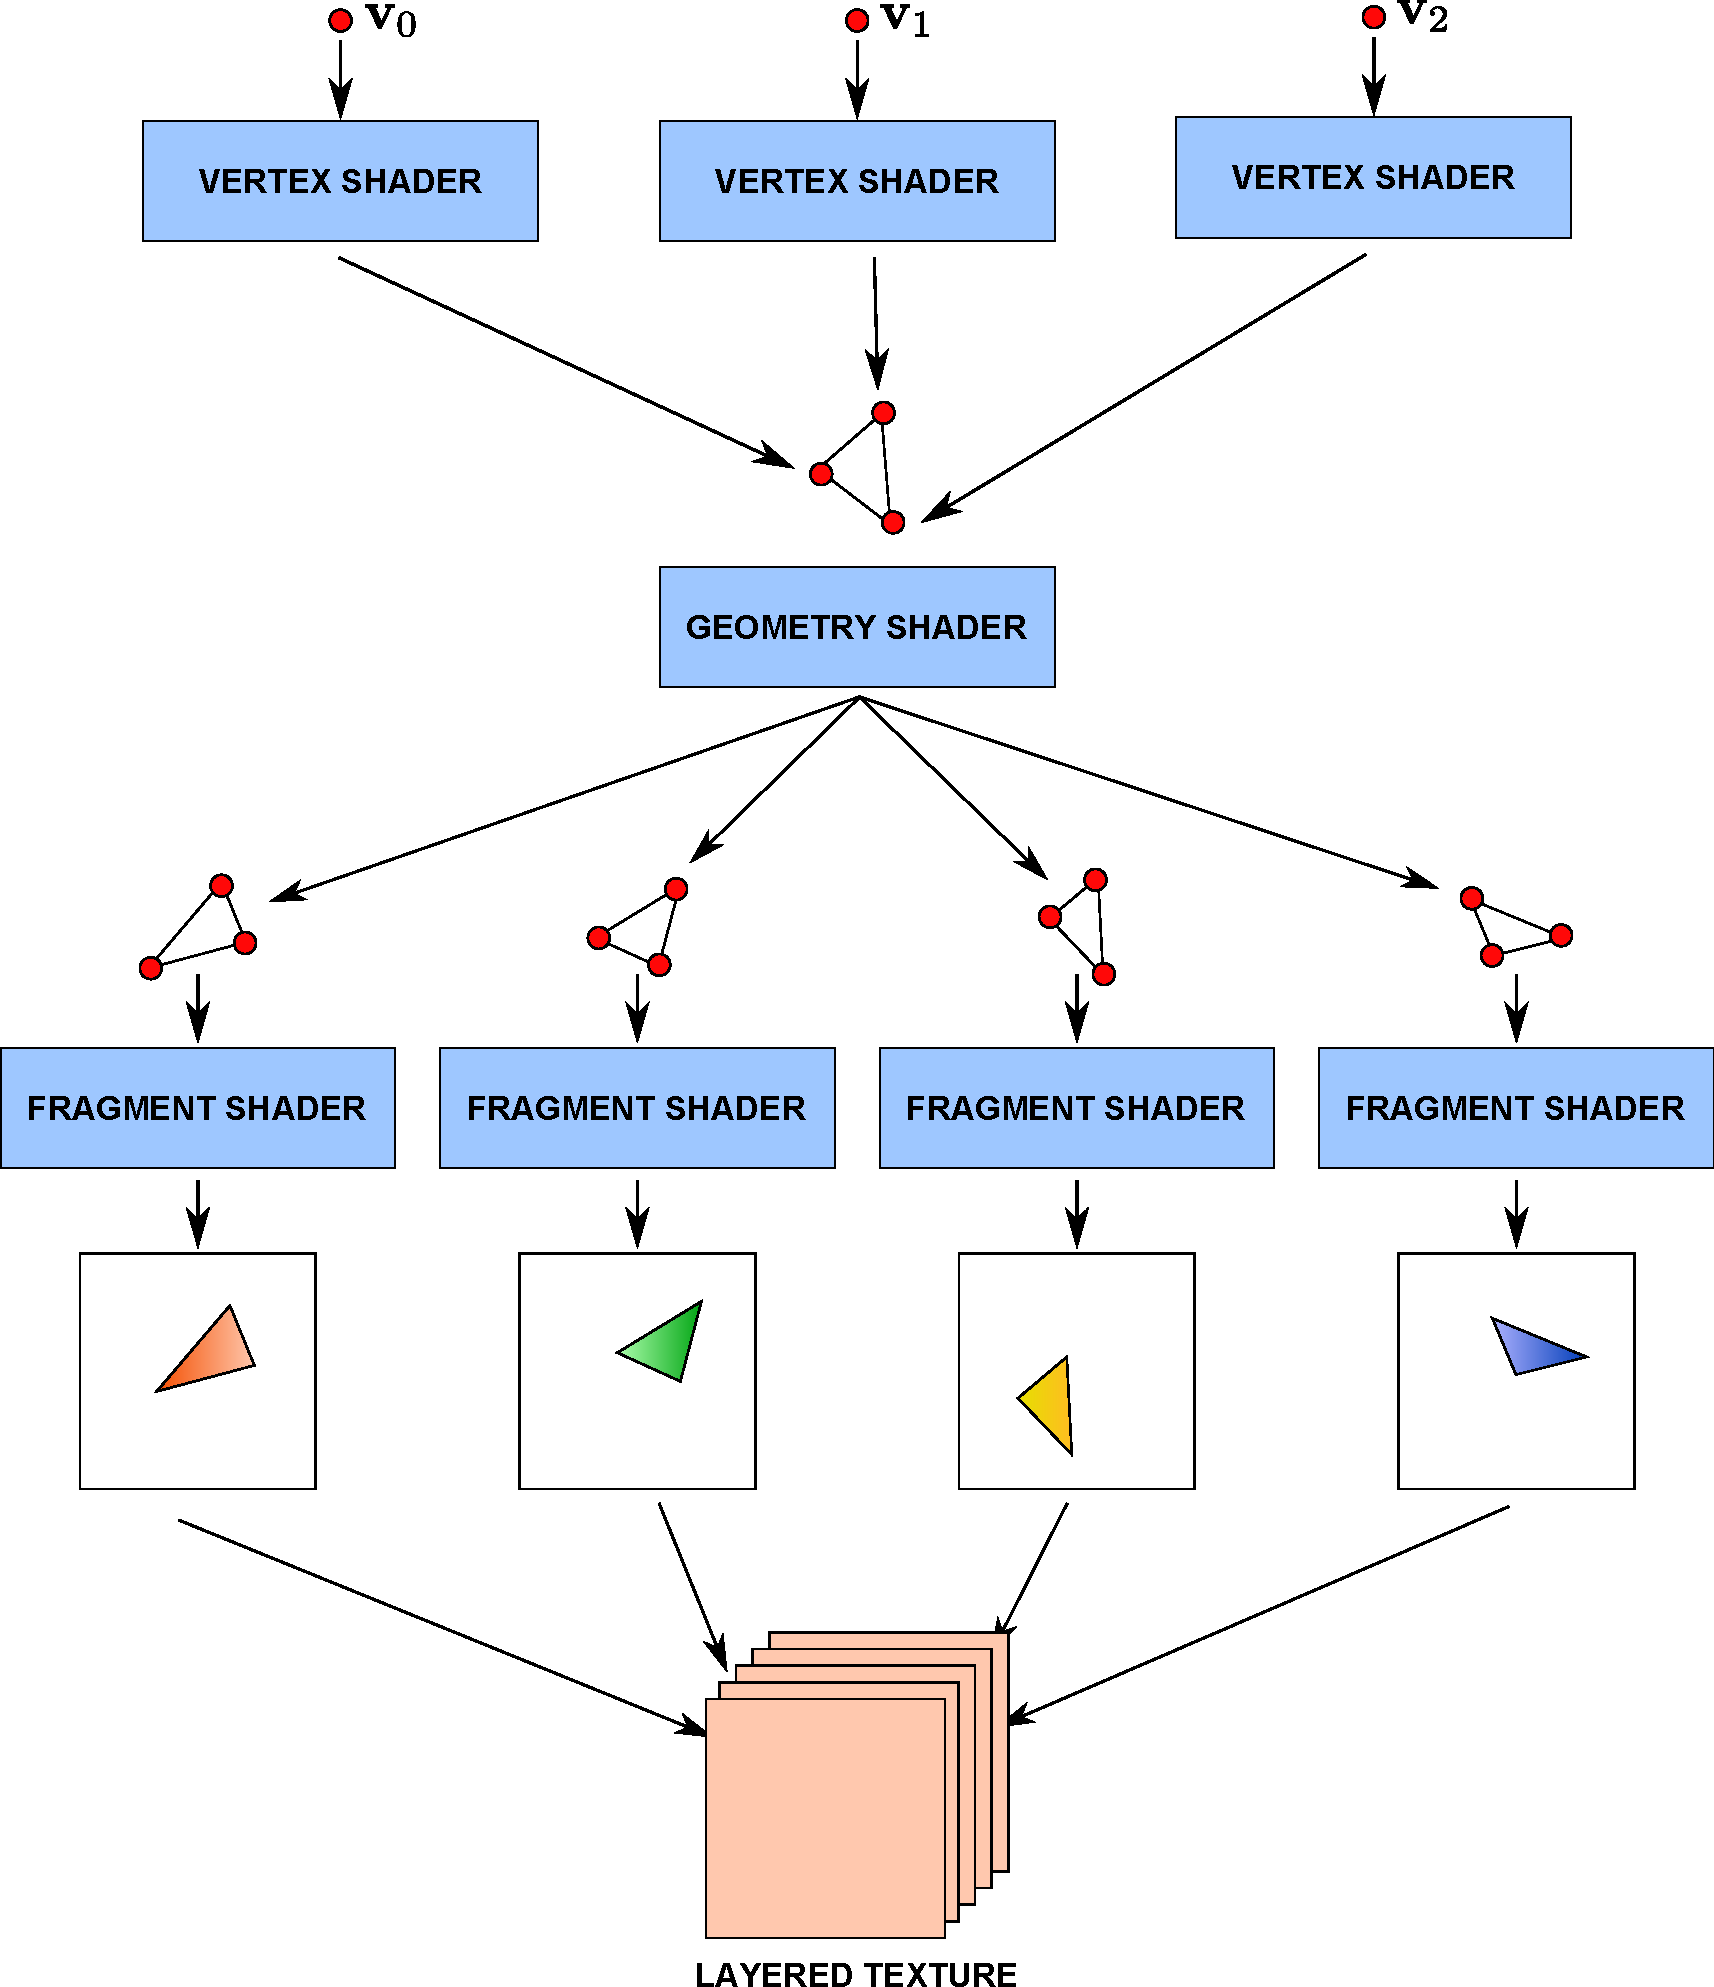
\includegraphics[width=\linewidth]{images/method/layered.pdf}
\caption{Diagram that illustrates layered rendering.}
\label{fig:layered}
\end{figure} 

We will use the OpenGL provided type \gl{GL_TEXTURE_2D_ARRAY}, that we initialize in the usual way, noting that an array texture should be initialized as a 3D texture. When binding it to an FBO, we use the generic \gl{glBindFramebufferTexture}:

\begin{lstlisting}[language=C++,label=lst:initarraytexture,caption={Initializing array texture. Note that the number of layers is passed to the \gl{glTexStorage3D} command.}]
GLuint fbo, arraytex;
glGenFramebuffers(1,&fbo);
glGenTextures(1, &arraytex);

glBindTexture(GL_TEXTURE_2D_ARRAY, arraytex);
[...] // setting up texture parameters, omitted
glTexStorage3D(GL_TEXTURE_2D_ARRAY, levels, GL_RGBA32F, size, size,layers);

glBindFramebuffer(GL_DRAW_FRAMEBUFFER, fbo);
glFramebufferTexture(GL_DRAW_FRAMEBUFFER, GL_COLOR_ATTACHMENT0, arraytex, 0);
\end{lstlisting}

In order to render to a layered texture, we need then to introduce a geometry shader. In our example, the difference between each layer is basically a different view matrix. So, we move the computation of the position, usually left to the vertex shader, to the geometry shader. We first introduce the code:

\begin{lstlisting}[language=GLSL,label=lst:arraygeomshader,caption={Geometry shader for layered rendering. The multiplication by the model matrix of vertex v is performed in the vertex shader (not shown).}]
#version 430
#define DIRECTIONS 16
layout(triangles) in;
layout(triangle_strip, max_vertices = 60) out;

uniform mat4 P;
uniform mat4 viewMatrices[DIRECTIONS];

void main(void)
{
    for(int i = 0; i < DIRECTIONS; i++)
    {
        gl_Layer = i;

        for(int k = 0; k < 3; k++)
        {
            vec4 v = gl_in[k].gl_Position;
            gl_Position = P * viewMatrices[i] * v;
            EmitVertex();
        }
        EndPrimitive();
    }
}
\end{lstlisting}

As we can see, we duplicate each one of the incoming triangles and then output it multiplied by a different view matrix. the \gl{EndPrimitive()} function ensures that the output triangles in the final triangle strip are separated. In order to render to a different layer each triangle, we need to set the special \gl{gl_Layer} variable to the layer we want to render before emitting the triangle. The whole process is illustrated in figure \ref{fig:layered}.

\subsection{Accumulation buffers}
\label{sec:accumulation}
Often, during the rendering process, we would like to accumulate the result of a computation, in order to progressively update the result of the computation. In order to do this, we encounter an obstacle: we would like to render to the currently bound texture, but at the same time we need to read the previous value stored on the texture. Unfortunately, the OpenGL Specification \citep{openglspec} advices against reading from the same texture we are rendering to. This is made to avoid a situation called \emph{feedback loop}. In fact, we cannot be sure of the results of what is stored in any pixel of the texture while we are rendering to it. 

There are many possible solutions to the problem. The first approach is to rely on the driver implementation: some drivers, in fact, allow to render to the same texture we are bound to, under some conditions. However, if we want a general method that works over all platforms, this is not a viable path. The second solution is to use image textures, a new type introduced in OpenGL 4.2 that allows explicit load-store of values, as well as new special constructs for GPU memory management (atomic operations and memory barriers). Though the usage of these features is appealing, their performance is generally poor compared to a framebuffer-based implementation. 

The final approach, and the one we describe in this chapter, is to use a technique called ping-pong. The idea is to sacrifice memory space by employing two textures $T_1$ and $T_2$. In the first frame, we render to the first texture $T_1$. IN the second frame, we use $T_2$ as a render target, and we sample $T_1$ and add it to the computed result. In the third frame, we render to $T_1$ and sample from $T_2$, and so on. From this alternance between the textures comes the name ping-pong. A minimal example of ping-ponging using a 2D texture is shown in listing \ref{lst:pingpong}.

\begin{lstlisting}[language=C++,label=lst:pingpong,caption={Minimal example of ping-pong textures.}]
// A global frame variable is initialized in order to keep track of the current frame

GLuint fbo, tex1, tex2;
// Creating FBO, initializing textures and texture parameters.
// Also binding shader with glUseProgram in order to bind texture uniforms
[...]

GLuint tex_from, tex_to;

tex_from = (frame % 2 == 0)? tex1 : tex2;
tex_to = (frame % 2 == 0)? tex2 : tex1;

glBindFramebuffer(GL_DRAW_FRAMEBUFFER, fbo);
glFramebufferTexture(GL_DRAW_FRAMEBUFFER, GL_COLOR_ATTACHMENT0, tex_to, 0);
glDrawBuffer(GL_COLOR_ATTACHMENT0);

GLint location = glGetUniformLocation("source_texture");
glUniform1i(location, 0);
glActiveTexture(GL_TEXTURE0);
glBindTexture(GL_TEXTURE_2D, tex_from);

// more uniforms and rendering commands.
[...]

frame ++;
\end{lstlisting}

\subsection{Generation of uniformly distributed points}
\label{sec:random}
In our method we have at least twice the necessity to generate uniformly distributed points either on a disc or on a sphere. To do this, we employ a particular sequence of pseudo-random numbers, called \emph{Halton points} \citep{Halton:1964:ARQ:355588.365104}. We explain briefly the ideas behind the sequence. For a more mathematical complete discussion on its properties of pseudo randomness, see \cite{niederreiter1992a}. 

First, given a prime number $p$ and a nonnegative integer $n$, we can express it in base $p$ as:
$$
n = a_0 + {a_1} p + a_2 p^2 + ... + a_r p^r
$$  

Where $a_i \in [0, p - 1]$. We now define a van der Corput sequence $\Phi_p(n)$ as:

$$
\Phi_p(n) = \sum_{i = 0}^r \frac{a_i}{p^{i+1}} = \frac{a_0}{p} + ... + \frac{a_r}{p^r}
$$

This sequence, given te fact that is based on prime points, automatically assumes good qualities of randomness. In addition, the function is already normalized in the range $[0,1)$. We define an Halton point as the combination of two Van der Corput sequences:

$$
H_{p_1,p_2}(n) = (\Phi_{p_1}(n), \Phi_{p_2}(n))
$$ 

Where $p_1$ and $p_2$ are two prime numbers, with $p_1 < p_2$. Usually, $(p_1,p_2) = (2,3)$ gives good results. All Halton points belong to the region of space $[0,1]\times[0,1]$. In order to obtain a sampling of Halton points on a sphere, we convert them using an area-preserving cartesian-to-spherical coordinates formula:

\begin{equation*}
\begin{split}
&H_{p_1,p_2}(n) = (\Phi_{p_1}(n), \Phi_{p_2}(n)) \rightarrow (s,t) \Rightarrow \\
&\Rightarrow H^{sphere}_{p_1,p_2}(n) = (\sqrt{1 - (2t - 1) ^2} \cos(2\pi s),\sqrt{1 - (2t - 1) ^2} \sin(2\pi s), 2t-1) 
\end{split}
\end{equation*}

And, to get the point on a disc, we simply take the point on a sphere and project it. In practice, we put the third coordinate to zero:

\begin{equation*}
\begin{split}
&H_{p_1,p_2}(n) = (\Phi_{p_1}(n), \Phi_{p_2}(n)) \rightarrow (s,t) \Rightarrow\\
& \Rightarrow H^{disc}_{p_1,p_2}(n) = (\sqrt{1 - (2t - 1) ^2} \cos(2\pi s),\sqrt{1 - (2t - 1) ^2} \sin(2\pi s)) 
\end{split}
\end{equation*}

\cite{journals/jgtools/WongLH97} provide an introduction to Halton points, as well as describing an implementation to generate a point on a Van der Corput sequence. We implemented their pseudo-code in C++ as follows:

\begin{lstlisting}[language=C++,label=lst:vandercorput,caption={Generating the p-adic Van der Corput point.}]
float vanDerCorputPoint(int n, int basis)
{
    int kp = n;
    float pp = (float)basis;
    float phi = 0.0f;
    while(kp > 0)
    {
        int a = kp % basis;
        phi = phi + a / pp;
        kp = int(kp / basis);
        pp = pp * basis;
    }
    return phi;
}
\end{lstlisting}

\begin{figure}[!ht]
\centering
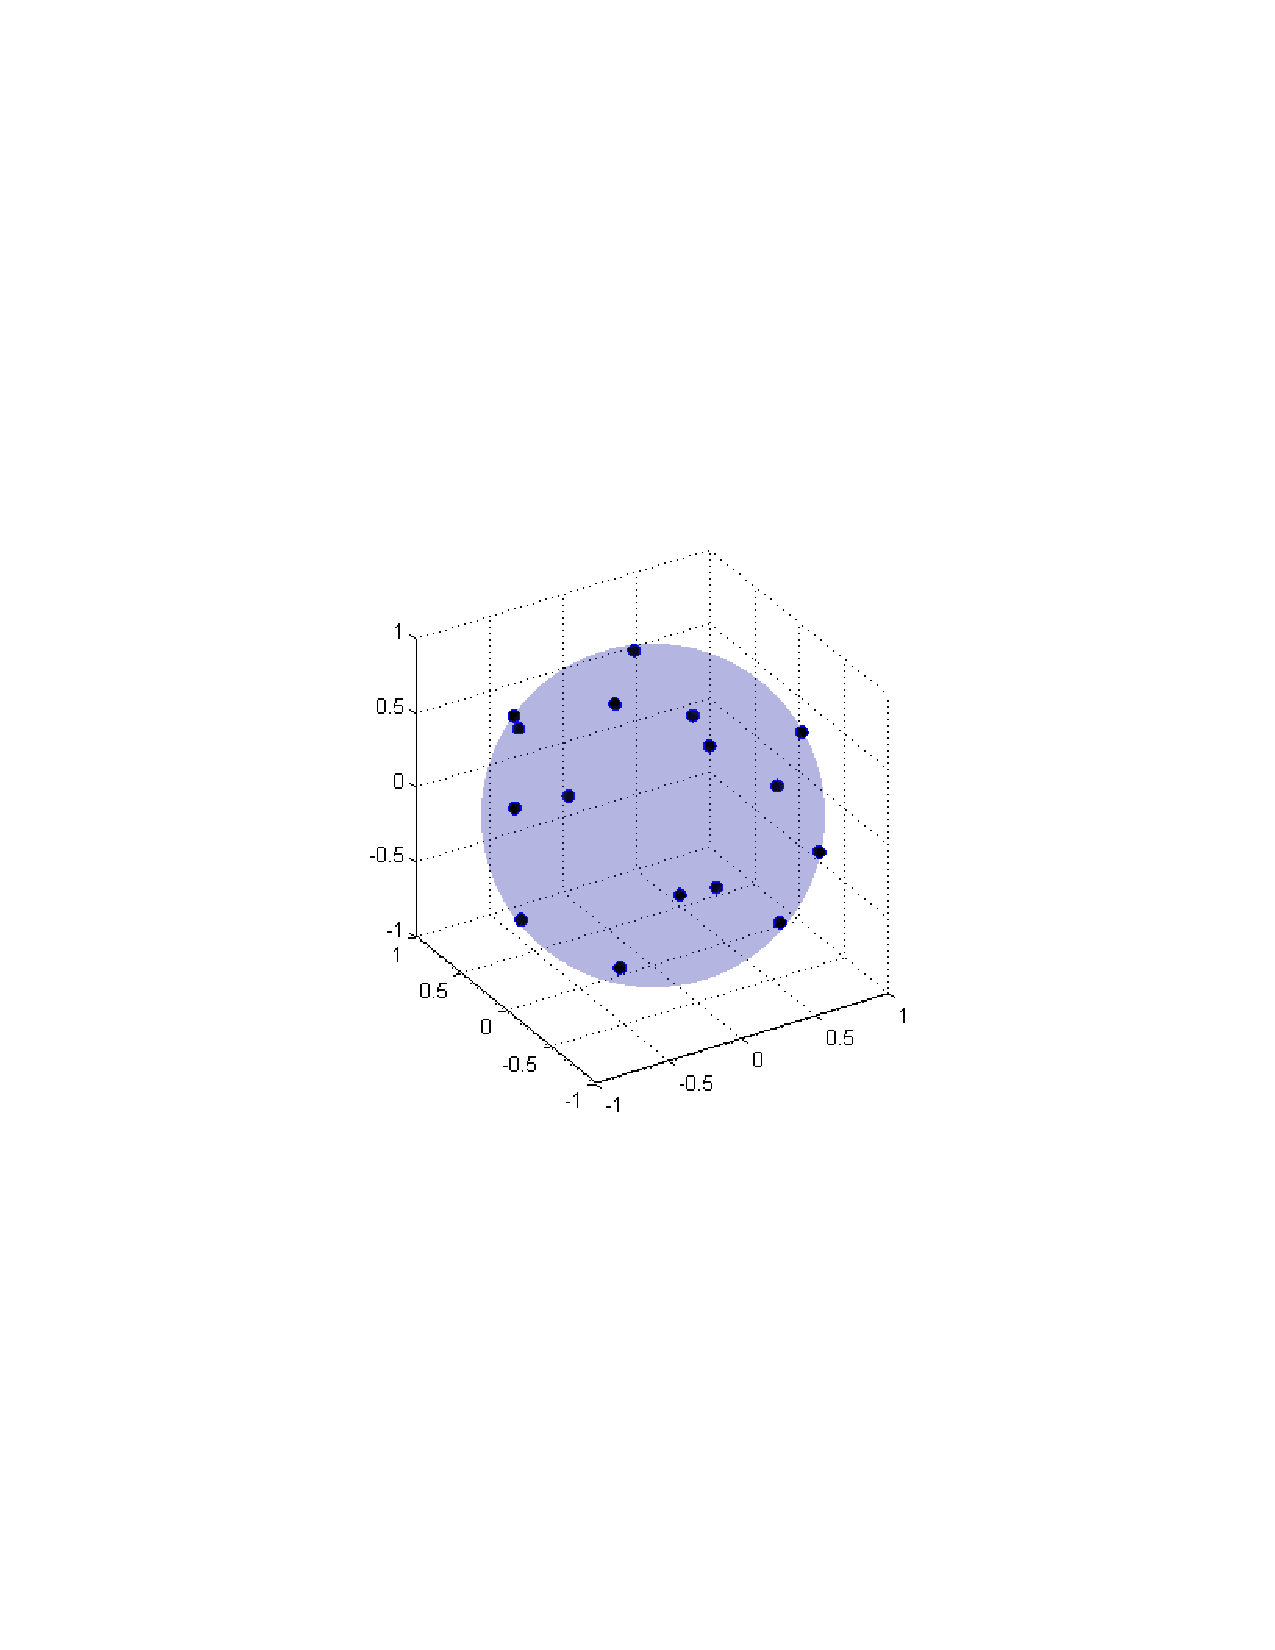
\includegraphics[width=0.5\linewidth]{images/matlab/cameras.pdf}
\caption{Positions of the first 16 cameras generated using Halton points on a sphere.}
\label{fig:cameras}
\end{figure} 

\subsubsection{Exponentially biased points}
\label{sec:exponentiallybiased}
In our algorithm, in order to obtain a better sampling, we need to have an exponentially biased distribution of points, as described in section \ref{sec:patterns} in the method chapter. To obtain this disc, we employ a technique called rejection sampling. The general idea is to generate a the sequence of halton points, then calculate their radius $r$ and calculate its probability distribution function using a coefficient $\sigma_{tr}$. Then, we use the following acceptance criterion:

$$
e^{-\sigma_{tr} r} > \zeta
$$

Where $\zeta \in [0,1)$ is a pseudo-randomly generated number. We can see that if the point is close to the center ($r \rightarrow 0$), $e^{-\sigma_{tr} r} \approx 1$ and so the point is more probable to be accepted. On the other hand, if the point is far from the center of the disc ($r \rightarrow +\infty$), $e^{-\sigma_{tr} r} \approx 0$ and so the point is less probable to be accepted. The code for generating a vector of accepted points is reported in listing \ref{lst:randomexp}.

\begin{lstlisting}[language=C++,label=lst:randomexp,caption={Generation by rejection of a exponentially distributed disc. The function generates $M$ points with distribution $e^{-\sigma_{tr} r}$, and where \gl{radius} is the maximum final radius of the points.}]
void planeHaltonCircleRejectionExponential(std::vector<Vec2f> &result, int m, float sigma_tr, float radius)
{
   uint accepted = 0;

   gel_srand(0);
   int i = 1;
   while(accepted < m)
   {
        Vec2f point = haltonPointCircle(i, 2, 3);
        float rad = point.length() * radius;
        float expon = exp(-sigma_tr * rad);
        float zeta = gel_rand() / ((float)(GEL_RAND_MAX));
        if(zeta < expon)
        {
            result.push_back(radius * point);
            accepted++;
        }
        i++;
   }
}
\end{lstlisting}

In our algorithm, we generate a number of samples $M$ that is fixed, with a radius equal to the size of the bounding box of the model. Then in the actual calculation only the $N$ points closest to $\x_o$ are actually used, allowing us to tweak the performance and the result. Moreover, the value of the exponent we pass to this method is not the true $\sigma_{tr}$. We pass a modified one according to the formula:

$$
q \sigma_{tr}
$$

Where $q$ is a parameter tweakable from the user. The idea is that the user can modify the distribution of the points, making them span a wider area (that is for $q > 1$) without increasing the number of samples $N$. In fact, a bigger $N$ implies a worse performance, while a bigger $q$ requires only to recompute the points. The problem of increasing $q$ too much is that some effects may be lost since we are not sampling close enough to the exitance point. We will leave this discussion on the parameters to chapter \ref{chap:results}. 

\begin{figure}[!ht]
\centering
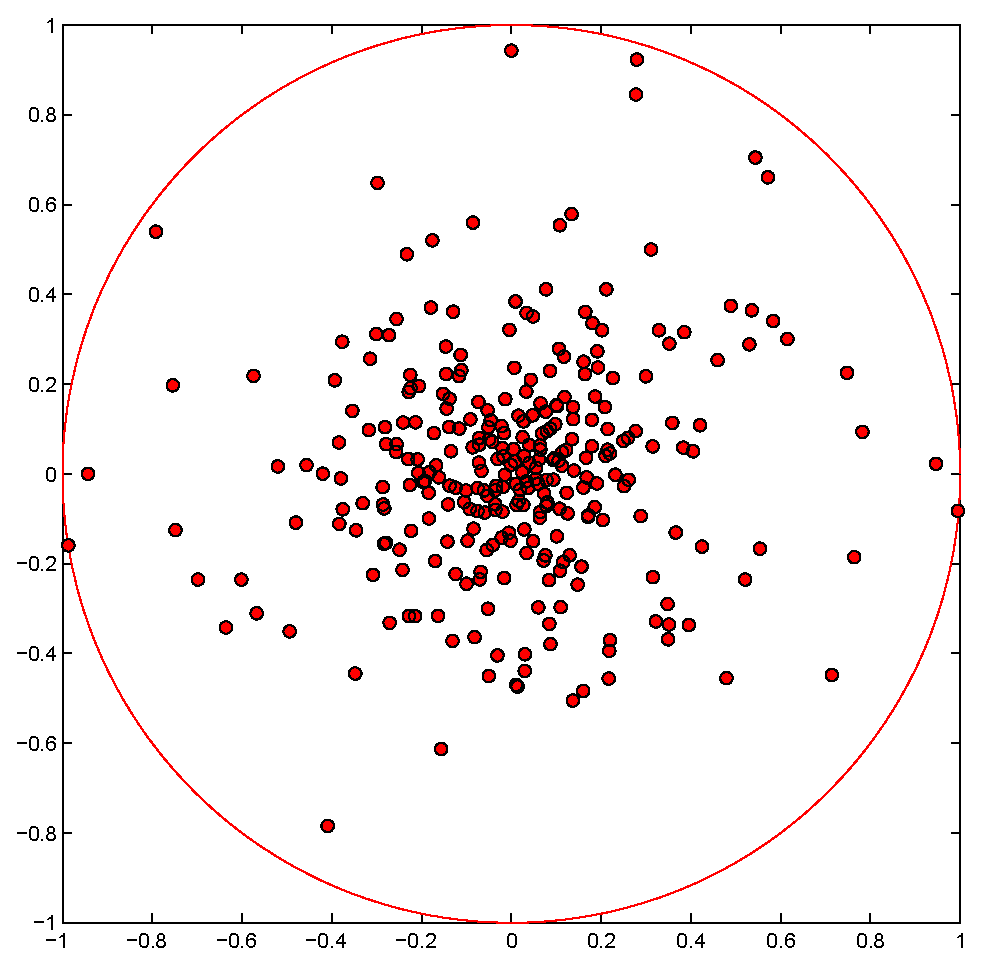
\includegraphics[width=0.7\linewidth]{images/matlab/halton_exp.eps}
\caption{Exponentially biased Halton points on a disk. The maximum radius is 1, and $M = 300$.}
\label{fig:hp}
\end{figure} 

\subsection{Shadow mapping}
\label{sec:shadow_map}
Shadow mapping is a common technique used in modern real-time graphics \citep{everitt,Segal:1992:FSL:142920.134071,williams1978a}. The idea behind it is to render an object from a light's point of view, and then use the generated depth information in order to decide if a point is shadowed or not. First of all, we convert the point into the light camera space, using a special space conversion matrix. After this, if we have a point $\mathbf{p} = (p_x,p_y,p_z)$, we compare $p_z$ to the texture $T$ sampled in the point $(p_x,p_y)$:

$$
p_z > T(p_x,p_y)
\label{eq:shadowtest}
$$ 

\begin{figure}[!ht]
\centering
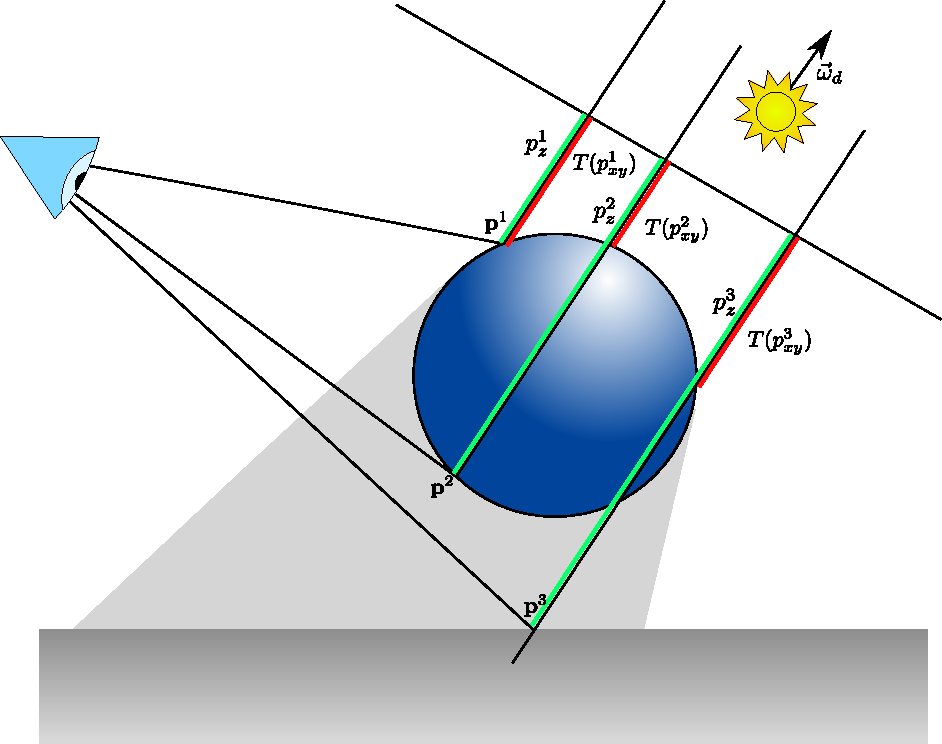
\includegraphics[width=\linewidth]{images/method/shadow_map.pdf}
\caption{Shadow mapping. We see the different results for three points $\mathbf{p^1}$, $\mathbf{p^2}$ and $\mathbf{p^3}$. The red length represents the value sampled from the depth texture($T(p_x,p_y)$), while the green length represents the value we compare against ($p_z$). When $p_z$ is less than $T(P_{xy})$, as in $\mathbf{p_1}$, the point is not shadowed. In the other cases, $\mathbf{p_2}$ and $\mathbf{p_3}$, $p_z > T(P_{xy})$and the point is not visible.}
\label{fig:shadow_map}
\end{figure} 

If the above condition is verified, it means that the current point is beneath the point visible from the light and then it should be shadowed. The matrix $L$ used to convert a point from world space to texture space is the following, using the matrix definitions and notation in section \ref{sec:matrices}:

$$
L = T\left(\frac{1}{2}\right) \cdot S\left(\frac{1}{2}\right) \cdot P \cdot V
$$

where $P$ and $V$ are the projection and view matrix we use to render with the light. The first two matrices are necessary to convert between clip and texture coordinates, as clip coordinates are in the range $[-1,1] \times [-1,1]$, while texture coordinates are in the range $[0,1]\times[0,1]$. The process is illustrated in figure \ref{fig:shadow_map}.

In our algorithm, we use the ideas behind shadow mapping in two different occasions. The first is to get the points $x_i$ in step 2 from the texture generated in step 1, where we use the matrix $L$ in order to convert the world point $\x_o$, corresponding to the pixel we are rendering to, into $\x_d$ the center of the disc in texture space. 

The second occasion is in the final combination step, where we use also shadow mapping in order to compute the visibility function $V^k(\x)$. Technically, the "light cameras` in this case are the directional cameras from where we render the scene, but the ideas behind are the same. We can see how we sample the shadow map in the final combination shader in the following listing:

\begin{lstlisting}[language=GLSL,caption={Sampling of the shadow map texture in step 3 of our method.}]
#version 430
uniform sampler2DArrayShadow depthMap;
uniform mat4 cameraMatrices[DIRECTIONS];

float sample_shadow_map(vec3 world_pos, int layer)
{
		vec4 light_pos = cameraMatrices[layer] * vec4(world_pos,1.0f);
    light_pos.z -= shadow_bias; //bias to avoid shadow acne
    if(light_pos.x < 0.0 || light_pos.x > 1.0) return 1.0;
    if(light_pos.y < 0.0 || light_pos.y > 1.0) return 1.0;
    return texture(depthMap,vec4(light_pos.x,light_pos.y,layer,light_pos.z)).r;
}        
[...] //shader code
\end{lstlisting}

In the above code, \gl{cameraMatrices[layer]} corresponds to the $L$ matrix. The special type of sampler \gl{sampler2DArrayShadow}, is a special sampler type that makes something more than its equivalent \gl{sampler2DArray}. The latter, in fact, accepts a \gl{vec3}, and simply retrieves the value in the texture. The former, on the other hand, accepts an extra parameter $z_{camera}$ (which is \gl{light_pos.z}), and compares it to the value stored in the depth texture $z_{tex}$, performing the test in equation \ref{eq:shadowtest}. If the depth of the point is less than the depth stored in the texture ($z_{camera} < z_{tex}$), 1 is returned as the point is closer to the directional camera, and thus visible. On the other hand, if $z_{camera} \ge z_{tex}$, it means the point is under the surface, and thus not visible, and 0 is returned.

To configure the \gl{sampler2DArrayShadow} texture, we need to specify some extra parameters during the depth texture initialization:

\begin{lstlisting}[language=C++,label=lst:textureconfshadow,caption={Configuration of a shadow map depth texture.}]
glBindTexture(GL_TEXTURE_2D_ARRAY, depthtex);
glTexParameterf(GL_TEXTURE_2D_ARRAY, GL_TEXTURE_MIN_FILTER, GL_NEAREST);
glTexParameterf(GL_TEXTURE_2D_ARRAY, GL_TEXTURE_MAG_FILTER, GL_NEAREST);
glTexParameterf(GL_TEXTURE_2D_ARRAY, GL_TEXTURE_WRAP_S, GL_CLAMP_TO_EDGE);
glTexParameterf(GL_TEXTURE_2D_ARRAY, GL_TEXTURE_WRAP_T, GL_CLAMP_TO_EDGE);
glTexParameterf(GL_TEXTURE_2D_ARRAY, GL_TEXTURE_COMPARE_MODE, GL_COMPARE_REF_TO_TEXTURE);
glTexParameterf(GL_TEXTURE_2D_ARRAY, GL_TEXTURE_COMPARE_FUNC, GL_LESS);
glTexStorage3D(	GL_TEXTURE_2D_ARRAY, 1, GL_DEPTH_COMPONENT32F, size, size, layers);
\end{lstlisting}

We can see that we specify two extra parameters: \gl{GL_TEXTURE_COMPARE_MODE}, once set to \gl{GL_COMPARE_REF_TO_TEXTURE}, means that sampling the depth texture in a shader will give a value based on the comparison between an extra value $z$ and the depth value $d$ in the texture. The second parameter \gl{GL_TEXTURE_COMPARE_FUNC} specifies how to compare the values: \gl{GL_LESS} means that 1 is returned if $z<d$, and zero is returned otherwise. 

\subsection{Memory layout}
\label{sec:memorylayout}

In this section, we briefly describe how memory is allocated in our method. The great advantage of using OpenGL 4.3 is that we can use \emph{texture views} \citep{openglspec}. Texture views are a way to create a texture in OpenGL, but on the opposite hand of \gl{glTexImage*D} or the \gl{glTexStorage*D} families of functions they allow for two texture to share the same storage on the GPU. To create a texture view, we use \gl{glTextureView}. We compare the standard way of allocating texture with our without texture view in figure \ref{fig:textureviews}.

\begin{figure}[h]
\centering
\subfloat[{Without texture views}]{
  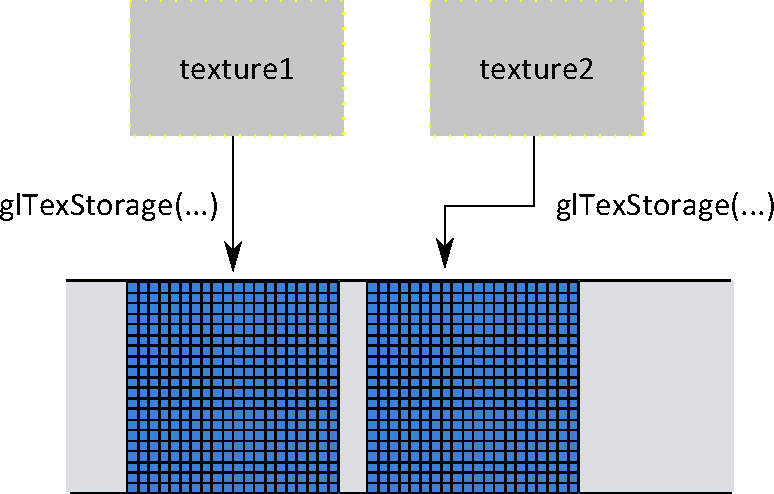
\includegraphics[width=0.5 \linewidth]{images/method/layout_no_view.pdf}
}
\subfloat[{With texture views}]{
  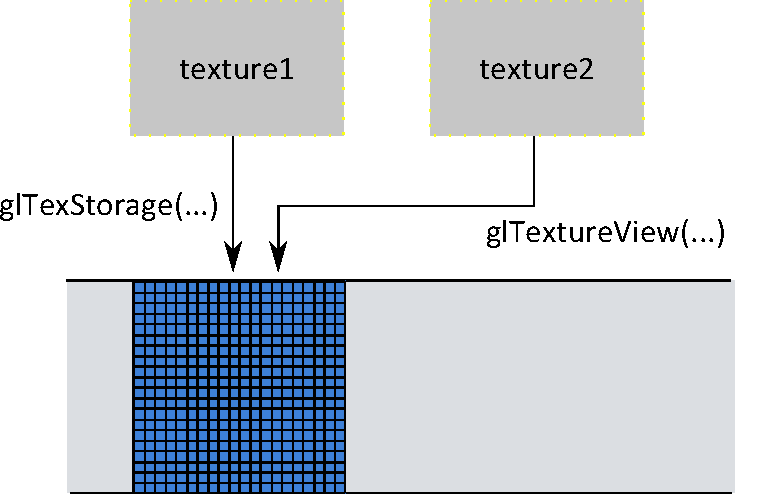
\includegraphics[width=0.5 \linewidth]{images/method/layout_view.pdf}
} 
\caption{Diagram illustrating texture views. On the top part of the picture the texture ids on the GPU, on the bottom the state of the memory. In the first case, we create two memory areas on the GPU using \gl{glTexStorage}, in the second case we make a single call to \gl{glTexStorage} and then a second call to \gl{glTextureView} to make them share the same storage space.}
\label{fig:textureviews}
\end{figure}


In our method, this comes to great advantages in two areas. First of all, since the depth map of the radiance map is not accumulated, we can make the two radiance maps share the same depth map. In addition, we can render directly between two mipmap levels of the same texture, something that we will need later to generate a blurred version of our texture.

A complete example memory layout for our algorithm is reported in table \ref{table:mlay}. As we will see, we will account for the contribution from multiple lights as more layers on the light map texture. More textures are loaded in order to make the method work, but their contribution is negligible.

\begin{table}[!h]
\centering
\begin{tabular}{p{3cm}lllll|l|}
\cline{2-7}
\multicolumn{1}{l|}{}                        & \multicolumn{1}{l|}{\textbf{Ch.}} & \multicolumn{1}{l|}{\textbf{Bits}} & \multicolumn{1}{l|}{\textbf{Width}} & \multicolumn{1}{l|}{\textbf{Height}} & \textbf{Depth} & \textbf{Size (MB)} \\ \hline
\multicolumn{1}{|l|}{Light map (vertex)}     & \multicolumn{1}{l|}{3}                 & \multicolumn{1}{l|}{32}                      & \multicolumn{1}{l|}{512}            & \multicolumn{1}{l|}{512}             & 1              & 3                  \\ \hline
\multicolumn{1}{|l|}{Light map (normals)}    & \multicolumn{1}{l|}{3}                 & \multicolumn{1}{l|}{32}                      & \multicolumn{1}{l|}{512}            & \multicolumn{1}{l|}{512}             & 1              & 3                  \\ \hline
\multicolumn{1}{|l|}{Light map (depth)}      & \multicolumn{1}{l|}{1}                 & \multicolumn{1}{l|}{32}                      & \multicolumn{1}{l|}{512}            & \multicolumn{1}{l|}{512}             & 1              & 1                  \\ \hline
\multicolumn{1}{|l|}{Radiance map 1 (color)} & \multicolumn{1}{l|}{4}                 & \multicolumn{1}{l|}{32}                      & \multicolumn{1}{l|}{512}            & \multicolumn{1}{l|}{512}             & 16             & 64                 \\ \hline
\multicolumn{1}{|l|}{Mipmaps 1}              & \multicolumn{1}{l|}{4}                 & \multicolumn{1}{l|}{32}                      & \multicolumn{1}{l|}{-}              & \multicolumn{1}{l|}{-}               & -              & 21                 \\ \hline
\multicolumn{1}{|l|}{Radiance map 2 (color)} & \multicolumn{1}{l|}{4}                 & \multicolumn{1}{l|}{32}                      & \multicolumn{1}{l|}{512}            & \multicolumn{1}{l|}{512}             & 16             & 64                 \\ \hline
\multicolumn{1}{|l|}{Mipmaps 2}              & \multicolumn{1}{l|}{4}                 & \multicolumn{1}{l|}{32}                      & \multicolumn{1}{l|}{-}              & \multicolumn{1}{l|}{-}               & -              & 21                 \\ \hline
\multicolumn{1}{|l|}{Radiance map (depth)}   & \multicolumn{1}{l|}{1}                 & \multicolumn{1}{l|}{32}                      & \multicolumn{1}{l|}{512}            & \multicolumn{1}{l|}{512}             & 16             & 16                 \\ \hline
                                             &                                        &                                              &                                     &                                      &                & \textbf{193 MB}       \\ \cline{7-7} 
\end{tabular}
\caption{Memory occupation of our method, for one light. Mipmaps are accounted for one additional third on the size of the radiance map. "Ch.` is the number of channels in the texture, "Bits` is the number of bits per channel.}
\label{table:mlay}
\end{table}

If we name some of the parameters, such as $L$ as the number of lights, $W_l$ the size of the light map, $K$ the number of directions and $W_s$ the size of the radiance map, we can obtain a direct formula to calculate the memory consumption in bytes:

$$
4 \left\{ \left[\left(4 + 4\right) \frac{4}{3} + 1\right] K W_s^2 + \left[3 + 3 + 1\right] L W_l^2 \right\}
$$

The $4/3$ factor account for the extra space reserved for mipmaps. The 4 factor at the beginning is because of each channel involved has 32 bits, that equal to 4 bytes. 

\section{Caveats}
The algorithm described so far, if implemented \emph{as is}, unfortunately does not give a result that we can appreciate. In order to obtain the desired result, some extra corrections are necessary.

\subsection{Random rotation of samples}

\begin{figure}
\centering
\subfloat[Constant rotation]{
  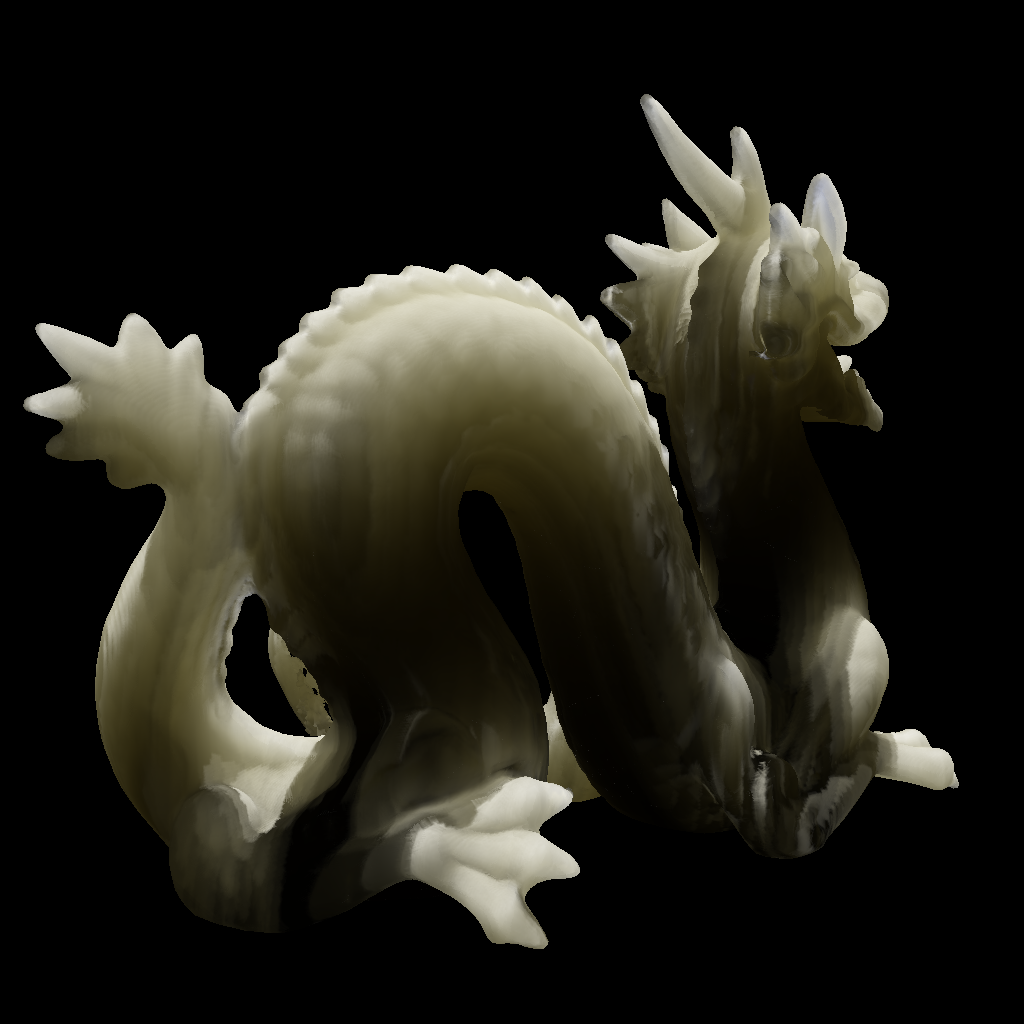
\includegraphics[width=0.5 \linewidth]{images/results/banding.png}
  \label{fig:banding1}
} 
\subfloat[Random rotation]{
  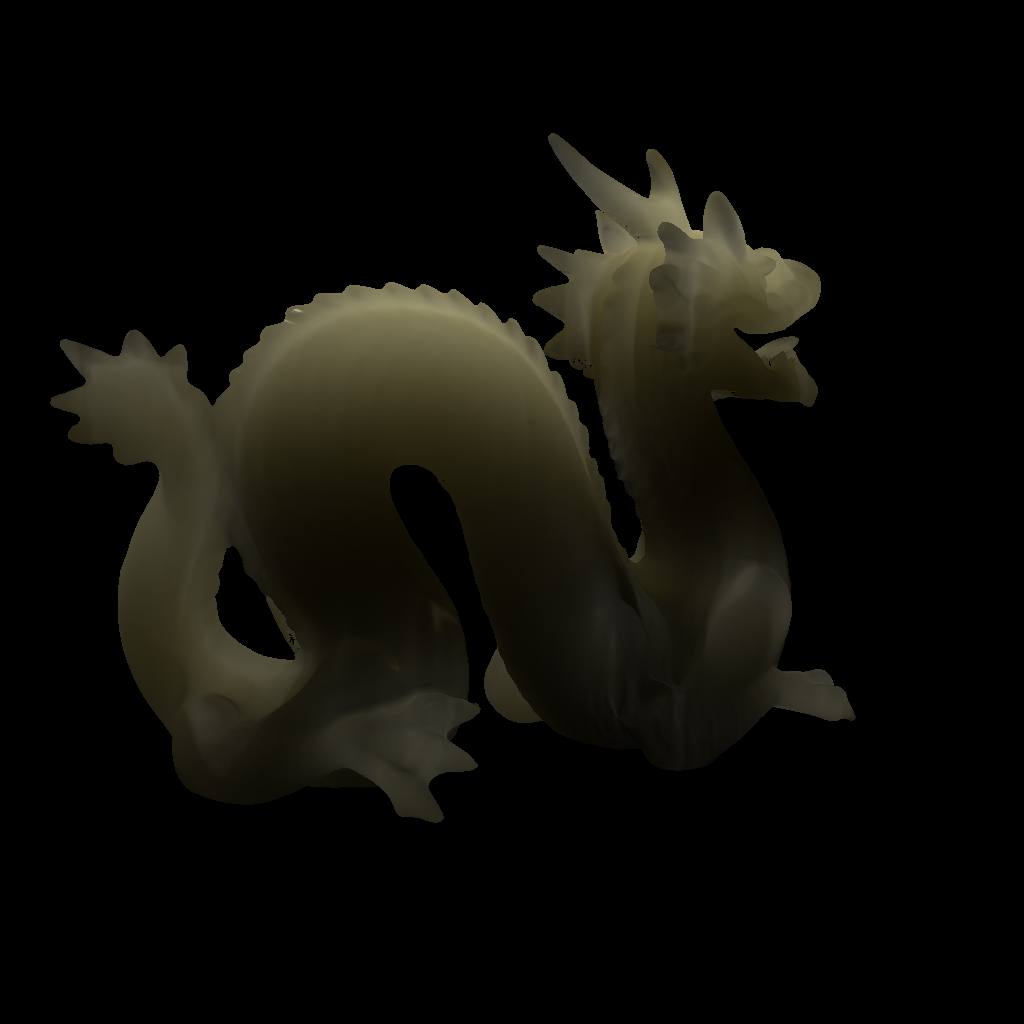
\includegraphics[width=0.5 \linewidth]{images/results/nobanding.png}
  \label{fig:banding2}
}  
\caption{White grapefruit juice dragon. The only difference in the two images is that the samples on the right figure are randomly rotated.}
\label{fig:banding}
\end{figure}

As we note in equation \ref{eq:evolution_step}, we never specified how the points in the samples are processed before actually being used in the calculation. This can lead to the assumption that the same disc pattern is used on every pixel. This causes a problem because this tends to generate banding artifacts, as we can see in figure \ref{fig:banding}. In order to avoid the artifacts, in exchange for noise, is to randomly rotate the pattern per pixel. Given that we are able to generate a random point $r$, we can take each one of the samples on the disk $\mathbf{d}_i$ and rotate it in order to obtain the new sample $\mathbf{d}_i^*$:

\renewcommand{\arraystretch}{1}
\begin{equation}
\begin{split}
\theta &= 2 \pi r \\
\mathbf{d}_i^* &= \left(\begin{array}{cc}
\cos\theta & \sin\theta \\
-\sin\theta & \cos\theta \\
\end{array} \right) \ \mathbf{d}_i
\end{split}
\label{eq:randomrot}
\end{equation}
\renewcommand{\arraystretch}{1.8}

Even if noisy, this result does not have any artifacts. We will see how to reduce the noise using mip maps in section \ref{sec:mipmaps}. As we observed before in the overview, we also need the result to evolve on a time basis, in order not to compute the same results on every frame. Recalling that the current frame is $t$ and the maximum amount of frames before we stop the computations is $T$, we make our computation evolve using the following $\theta_t$ in equation \ref{eq:randomrot}:

$$
\theta_t = 2 \pi \left(r + \frac{t}{T}\right)
$$

This causes a progressive rotation of the disc around the point over time. However, we need still to specify how to calculate $r$. As a function, $r = (x,y,l)$ needs to depend on the fragment coordinates $(x,y)$, as well as from the current layer $l$ (to avoid two layers make the same computation). Since we are on the GPU, we cannot use a built-in random function, so we need either to load the random points from the CPU as a separate texture or to generate them on-the-fly. For the latter technique, we tried a sine based generator, a linear shift (LSR) random generator and a congruential linear generator (LCG), all in listing \ref{lst:sinegenerator}. The input point that was given was in both cases $(l \cdot x, l \cdot y)$. We can see some results in figure <ref{fig:noises}. The sine based generator theoretically gives the best result, but the linear shift generator gives an indistinguishable result.

\begin{figure}
\centering
\subfloat[Sine noise]{
  
\includegraphics[width=0.33 \linewidth]{images/method/noise_1.png}
  \label{fig:noise1}
} 
\subfloat[LSR noise]{
  
\includegraphics[width=0.33 \linewidth]{images/method/noise_2.png}
  \label{fig:noise2}
} 
\subfloat[LCG noise]{
  \includegraphics[width=0.33 \linewidth]{images/method/noise_3.png}
  \label{fig:noise3}
}  
\caption{Three examples of deterministic noise generation on GPU. While the sine and linear shift noises give a uniform and pleasant noise, the linear congruential generator has a periodicity.}
\label{fig:noises}
\end{figure}

\begin{lstlisting}[language=GLSL,label=lst:sinegenerator,caption={Three GLSL functions to generate random points on the GPU. The extra size parameter is the height of one layer of the radiance map texture.}]
highp float noise_sine(vec2 co)
{
    highp float a = 12.9898;
    highp float b = 78.233;
    highp float c = 43758.5453;
    highp float dt = dot(co.xy,vec2(a,b));
    highp float sn = mod(dt,3.14);
    return fract(sin(sn) * c);
}

highp float noise_lsrg(vec2 co, int size)
{
		int n = co.x + size * co.y;
    n = (n << 13) ^ n;
		int s = (n * (n*n*15731+789221) + 1376312589) & 0x7fffffff;
		return s / (4294967296.0f) * 2;
}

highp float noise_lcg(vec2 co, int size)
{
		int n = co.x + size * co.y;
		return float((n * 1664525 + 1013904223) % 4294967295) / 4294967296.0f;
}
\end{lstlisting}



\subsection{Mipmap generation}
\label{sec:mipmaps}
The randomization we performed in the previous step comes with a drawback, i.e. we increase the noisiness of the result, especially in the initial steps. Once we reach convergence, the noisiness slowly disappears. In order to improve our method, we need to introduce a way to take the intermediate result and make it as close as possible to the final result at convergence. Our approach was to use a filter to blur the result multiple times, storing the results in the mipmaps of the radiance map generated in step 2 of our method. This results in an additional step between step 2 and step 3, where the mip maps are calculated.

We tried different filters with different weights, and we will test some of them in the result chapter. The one that gave us the most promising results is the bilinear filter with the shape shown in figure \ref{fig:filters}. The filter uses the alpha value of the texture as a weight for the sampled color, so the filter maintain the edges of the texture. %if time --> We can see in figure TODO a comparison between the standard mipmap filter (which is an averaging of four neighbouring pixels) and our bilinear filter, noticing immediately the result.

\begin{figure}
\centering
\subfloat{
  \includegraphics[width=0.33 \linewidth]{images/method/filter_1.pdf}
  \label{fig:filter1}
} 
\subfloat{
  \includegraphics[width=0.33 \linewidth]{images/method/filter_2.pdf}
  \label{fig:filter2}
} 
\subfloat{
  \includegraphics[width=0.33 \linewidth]{images/method/filter_3.pdf}
  \label{fig:filter3}
}  
\caption{Alpha-weighted bilinear filter. In \ref{fig:filter1} we have the shape of the filter. In \ref{fig:filter2} we have the alpha channel of an example image, to which we show the weights used in the filters in figure \ref{fig:filter3}, based on the alpha channel of the picture.}
\label{fig:filters}
\end{figure}

On the implementation level, the mipmaps need to be rendered one after the other, as we need the result of the first computation in order to perform the second. So, we use always the same shader, reported in listing \ref{lst:shaderimageprocessing}, to filter between two textures. In the first step, we bind layer zero (where the result of the rendering of step 2 is stored) as source and layer one as destination. Then, we bind layer 1 as source and layer 2 as destination, and so on. To perform the filtering, we render a full screen quad.

However, OpenGL does not allow to bind the same image both as a source and as a destination, even if the mipmap levels are different. So, in order to overcome this difficulty, we use texture views as we described them in \ref{sec:memorylayout}. We create a new texture for the mipmaps, but then we configure it to use the storage reserved to the mipmaps of the radiance map. So, we can bind it to the FBO as it was a completely different texture, but then once we render the result will be rendered in the right memory location. % if time --> Figure TODO offer a visual explanation.

\begin{lstlisting}[language=GLSL,label=lst:shaderimageprocessing,caption={Custom mipmap filtering on GPU. \gl{_tex} are the texture coordinates on the screen aligned quad.}]
#version 430
in vec3 _tex;
uniform sampler2DArray source;

out vec4 fragColor;

uniform float texStep;
uniform int scaling;

void main(void)
{
	int layer = gl_Layer;
	float t_step = texStep * 0.5 * scaling;
	vec4 c0  = texture(source,vec3(_tex.xy,layer));
	vec4 c1  = texture(source,vec3(_tex.xy + vec2(t_step,0.0f),layer));
	vec4 c2  = texture(source,vec3(_tex.xy - vec2(t_step,0.0f),layer));
	vec4 c3  = texture(source,vec3(_tex.xy + vec2(0.0f, t_step),layer));
	vec4 c4  = texture(source,vec3(_tex.xy - vec2(0.0f, t_step),layer));

	vec4 c5  = texture(source,vec3(_tex.xy + 2 * vec2(t_step,0.0f),layer));
	vec4 c6  = texture(source,vec3(_tex.xy - 2 * vec2(t_step,0.0f),layer));
	vec4 c7  = texture(source,vec3(_tex.xy + 2 * vec2(0.0f, t_step),layer));
	vec4 c8  = texture(source,vec3(_tex.xy - 2 * vec2(0.0f, t_step),layer));

	vec4 c9  = texture(source,vec3(_tex.xy + vec2(t_step,t_step),layer));
	vec4 c10 = texture(source,vec3(_tex.xy - vec2(t_step,t_step),layer));
	vec4 c11 = texture(source,vec3(_tex.xy + vec2(t_step, -t_step),layer));
	vec4 c12 = texture(source,vec3(_tex.xy - vec2(t_step, -t_step),layer));

	float v0 = clamp(c0.a,0.0f,1.0f);
	float v1 = clamp(c1.a,0.0f,1.0f);
	[...] //omitted
	float v12 = clamp(c12.a,0.0f,1.0f);

	vec4 step1 = c0 * v0 + c1 * v1 + c2 * v2 + c3 * v3 + c4 * v4;
	float vstep1 = v0 + v1 + v2 + v3 + v4;
	vec4 step2 = c5 * v5 + c6 * v6 + c7* v7 + c8 * v8;
	float vstep2 = v5 + v6 + v7 + v8;
	vec4 step3 = c9 * v9 + c10 * v10 + c11 * v11 + c12 * v12;
	float vstep3 = v9 + v10 + v11 + v12;

	fragColor = (step1 + step2 + step3 )/max(vstep1 + vstep2 + vstep3, 1.0f);
}
\end{lstlisting}

\begin{figure}
\centering
\subfloat{
  \includegraphics[width=0.33 \linewidth]{images/results/mipmap_0.png}
  \label{fig:mip0}
} 
\subfloat{
  \includegraphics[width=0.33 \linewidth]{images/results/mipmap_1.png}
  \label{fig:mip1}
} 
\subfloat{
  \includegraphics[width=0.33 \linewidth]{images/results/mipmap_2.png}
  \label{fig:mip2}
}  \\
\subfloat{
  \includegraphics[width=0.33 \linewidth]{images/results/jeppe_noise.png}
  \label{fig:jenoise}
} 
\subfloat{
  \includegraphics[width=0.33 \linewidth]{images/results/jeppe_mipmap_1.png}
  \label{fig:jemip1}
} 
\subfloat{
  \includegraphics[width=0.33 \linewidth]{images/results/jeppe_mipmap_2.png}
  \label{fig:jemip2}
}  
\caption{Mipmap generation. On the first row, left to right, the base level and two subsequent applications of the bilinear filter (the images have been cropped for a better visualization). On the bottom row, the model sampled with the different mipmap levels. We note that at level 2 artifacts start to emerge along the camera seams.}
\label{fig:mipmaps}
\end{figure}


\subsection{Shadow bias}

The shadow mapping described in section \ref{sec:shadow_map} has an obvious problem, called \emph{shadow acne}. As we can see in figure \ref{fig:shadowbias}, the discretization of depth comes with a problem: depending on the incidence angle, the surface starts generating an alternating pattern of dark and light on the visible areas. The solution in this case is to introduce a constant factor when we are comparing the texture space position and the depth of a point, called \emph{shadow bias} $\epsilon_b$. The test then becomes:

$$
p_z - \epsilon_b < T(p_x,p_y)
$$ 

The result is depicted in figure \ref{fig:shadowbias}. As we can see, we raise the sampling by the bias factor, so the lit areas do not present shadow acne anymore. This comes with a drawback: the shadow bias, for thin objects, it introduces another artifact, called \emph{peter panning}, i.e. the shadow and the object become disconnected. In the case of our method, a too large bias makes the different directions to become "disconnected`, not representing a faithful result. 

\begin{figure}
\centering
\subfloat[Shadow acne]{
  \includegraphics[width=0.5 \linewidth]{images/method/shadow_bias.pdf}
  \label{fig:acne}
}
\subfloat[Shadow acne, with shadow bias]{
  \includegraphics[width=0.5 \linewidth]{images/method/shadow_bias_correct.pdf}
  \label{fig:bias}
} \\
\subfloat[Shadow acne, result]{
  \includegraphics[width=0.5 \linewidth]{images/method/acne.png}
  \label{fig:acneres}
}
\subfloat[Shadow acne, with shadow bias, result]{
  \includegraphics[width=0.5 \linewidth]{images/method/noacne.png}
  \label{fig:biasres}
}

\caption{Shadow acne (figure \ref{fig:acne}) origin: the angle of the light causes little bands to appear. Adding a small offset $\epsilon_z$ to the sampling (\ref{fig:bias}) corrects the result, leading to a full lit surface. On the bottom row, the two figures \ref{fig:acneres} and \ref{fig:biasres} show the results with and without the correction.}
\label{fig:shadowbias}
\end{figure}


\subsection{Texture discretization artifacts}
A problem related to the previous one is texture discretization artifacts, that appear as seams in the texture in figure \ref{fig:combias}. The problem is similar to the one of depth bias, but it manifests on the direction perpendicular to the directional cameras. Because of the discretization and the depth bias in the shadow sampling, some pixels become false positives, being incorrectly sampled even if they are not visible. To fix this, we apply a transformation to the vertex in the final step that shrinks it a little bit towards the center of the texture. The shrinking is made using the camera direction as a main axis, according to the formula:

$$
\x_o^{shrink} = \x_o - \epsilon_c (\vec{n}_o - \vomega_d (\vec{n}_o \cdot \vomega_d));
$$

Where $\epsilon_c = \frac{1}{W}$, where $W$ is the width of the radiance map in pixel. In this way we obtain a shrinkage of one pixel of the model when we use $\x_o^{shrink}$ for sampling the radiance map. As we can see in figure \ref{fig:combias}, adding this correction solves the problem.

\begin{figure}
\centering
\subfloat[Without correction]{
  \includegraphics[width=0.5 \linewidth]{images/results/comb_offset.png}
  \label{fig:comb_off}
}
\subfloat[With correction]{
  \includegraphics[width=0.5 \linewidth]{images/results/comb_offset_solved.png}
  \label{fig:comb_off_solved}
} 
\caption{Combination offset artifacts. Without the correction, artifacts start to appear. With a correction of $0.001 \approx 1 / 1024$ the result is greatly improved.}
\label{fig:combias}
\end{figure}


\section{Extensions to the method}

In this section, we describe briefly how we extended our implementation in order to cover a wider range of cases, especially regarding different types of light.

\subsection{Rendering with multiple lights}

\begin{figure}
\centering
\includegraphics[width=0.9 \linewidth]{images/results/multiple.png}
\caption{Rendering with two point lights. The material parameters used are for white grapefruit juice. One light comes from the left ($\vomega_l = (1,0,0)$), with radiance $L_d = (13,5,5)$. One comes from the top ($\vomega_l = (0,0,1)$), with radiance $L_d = (5,5,13)$.}
\label{fig:multilight}
\end{figure}

Rendering with multiple lights requires only a slight extension to the method. We just need to adjust the computation in \ref{eq:evolution_step} in order to account for multiple lights, obtaining a result as the one in figure \ref{fig:multilight}. We notice that this computation may come with a performance penalty, since we are now computing the contribution from $L N$ samples instead of $N$, where $L$ is the number of lights. To avoid this, we account in advance and calculate only $\frac{N}{L}$ samples per light:

$$
R^{t,k}(\x_o) = \sum_{l = 1}^L L_l \sum_{i = 1}^{N/L} S(\x^{t,k}_i, \vomega^t_l, \x_o, \vomega_o) \exp\left(\sigma_{tr} r^{t,k}_i\right), \ \ t \in [0,T], \ \ k \in [0,K-1] 
$$

We can see that only the light vector $\vomega^t_l$ and the radiance $L_l$ depend on the current light, while the other parameters are left unchanged. On the implementation level, we first need to change the light map in order to be a layered texture as well. As in step 2, we employ layered rendering to render all the faces at the same time. Then we simply add an extra loop in the shader of step 2. As for the light parameters, they are passed to the shader as a series of uniforms. The outline of the new shader illustrating how lights are computed is listed in listing \ref{lst:multi}.

\begin{lstlisting}[language=GLSL,label=lst:multi,caption={Outline of the shader in step 2 with support for multiple lights.}]
#version 430
layout(location = 0) out vec4 fragColor;

[...] // constants, includes, textures omitted

uniform sampler2DArray vtex; // texture with vertices
uniform sampler2DArray ntex; // texture with normals

smooth in vec3 position;
smooth in vec3 norm;

uniform vec4 light_pos[MAX_LIGHTS];
uniform vec4 light_diff[MAX_LIGHTS];
uniform int light_number;
uniform mat4 lightMatrices[MAX_LIGHTS];

[...] //BSSRDF code, uniform and functions

void main(void)
{
    vec3 xo = position;
    vec3 no = normalize(norm);

		[...] // sampling the old color, noise calculation

    for(int k = 0; k < light_number; k++)
    {
        vec3 wi = light_pos[k].xyz;
        vec4 light_post = lightMatrices[k] * vec4(xo,1.0f);
        vec2 circle_center = light_post.xy;
        vec3 Li = light_diff[k].xyz;
				
        for(int i = 0; i < max_samples; i++)
        {
						[...] // sampling from layer k in textures vtex and ntex
						[...] // summing over BSSRDF on vector accumulate
        }
    }

    fragColor = vec4(accumulate,1.0f);
		[...] //adding old color
}
\end{lstlisting}

\subsection{Rendering with other kinds of light}

Our method does not depend on a specific type of light in order to render a material. Once we have a formula for the radiance for the light, we can simply introduce it in equation \ref{eq:evolution_step} and compute the result. So, for example, for a point light the equation would become.

$$
R^{t,k}(\x_o) = {I_l} \sum_{i = 1}^N  \frac{S(\x^{t,k}_i, \frac{\x_l - \x_i}{\|\x_l - \x_i\|}, \x_o, \vomega_o)}{{\|\x_l - \x_i\|}} \exp\left(\sigma_{tr} r^{t,k}_i\right), \ \ t \in [0,T], \ \ k \in [0,K-1] 
\label{eq:evolution_step_2}
$$

Where $\x_l$ is the light position and $I_l$ the light intensity. More generally, if we have a function to compute the light direction $\vomega_l(\x_i)$ and a function to compute radiance $L(\x_i, \vomega_l(\x_i))$ we can express equation \ref{eq:evolution_step} in the following way:

$$
R^{t,k}(\x_o) = \sum_{l = 1}^L \sum_{i = 1}^{N/L} L^t(\x_i, \vomega_l(\x_i)) S(\x^{t,k}_i, \vomega_l^t(\x_i), \x_o, \vomega_o) \exp\left(\sigma_{tr} r^{t,k}_i\right)
$$

If we have only point and directional lights, we have the following setup for the two formulas:

\begin{equation*}
\begin{split}
\vomega_l(\x_i) &= \begin{cases}
\vomega_l & \text{if l is directional with $\vomega_l$, $L_l$} \\
 \frac{\x_l - \x_i}{\|\x_l - \x_i\|} & \text{if $l$ is point with $\x_l$, $I_l$}
\end{cases} \\
L(\x_i, \vomega_l(\x_i)) &= \begin{cases}
L_l & \text{if l is directional with $\vomega_l$, $L_l$} \\
 \frac{I_l}{\|\x_l - \x_i\|} & \text{if $l$ is point with $\x_l$, $I_l$}
\end{cases} \\
\end{split}
\end{equation*}

On the implementation level, we can still use same uniform setup for lights. We make the position vector of the light carry some extra information in the alpha channel: if the alpha is zero, we are dealing with a directional light, while if the alpha is one we are using a point light. The code to calculate lights thus becomes:

\begin{lstlisting}[language=GLSL,label=lst:multilighttype,caption={GLSL Code to calculate the radiance \gl{Li} and the incoming light direction \gl{wi} for the k-th directional or point light source.}]
int current_light = k;
vec3 wi = light_pos[current_light].xyz;
vec4 rad = light_diff[current_light];
vec3 topoint = wi - xo;
float light_type = light_pos[current_light].a;
wi = (light_type > 0)? normalize(topoint) : normalize(wi);
vec3 Li = light_diff[current_light].xyz;
Li = (light_type > 0)? Li / dot(topoint,topoint) : Li;
\end{lstlisting}

\begin{figure}
\centering
\subfloat[Directional:  $\vomega_l = (0,0,1)$ $L_d = (8,8,8)$]{
  \includegraphics[width=0.5 \linewidth]{images/results/directional.png}
  \label{fig:dir_light_ex}
}
\subfloat[Point:  $\x_l = (0,0,2)$  $I_d = (18,18,18)$]{
  \includegraphics[width=0.5 \linewidth]{images/results/point.png}
  \label{fig:point_light_ex}
} 
\caption{Rendering with a directional and a point light. The material parameters are the ones for potato.}
\label{fig:dir_point_comparison}
\end{figure}


\subsection{Rendering with environment light illumination}
\label{sec:envenv}
As for the environment lighting, we proceed as we outlined in section \ref{sec:env}. In the method chapter, we omitted how we do actually organize and sample our CDF. The idea is to have one CDF for the rows of the function that gives us the CDF according to the probability $p_u(u)$. Then we have a CDF for each one of the column of the functions, that sample the probability $p_v(v|u)$. When we select a random couple of random points $(\zeta_1,\zeta_2)$ we first sample the first function according to $\zeta_1$, then we sample the resulting column using $\zeta_2$.

We define our discreet CDF as and array $C$ of $s+1$ elements as follows, where $s$ is the size of the distribution $P$ (that would be either $n$ or $m$ in our case). $P$ is an array of $N$ elements.

$$
C[i] = \frac{\sum_{k = 0}^{i-1} C[k]}{s\ C[s]}
$$

Then, we sample our CDF using a generic value $\zeta$ using the following:

$$
u = j + \frac{\zeta - C[j]}{C[j + 1] - C[j]}
$$

Where $j = \min_j\{j \in [0,s] | C[j] > \zeta \} - 1$ is the CDF value right before the CDF surpasses $\zeta$. This is basically the inverse function we discussed in the chapter method. Once we have calculated the two values $(u_1,u_2)$, as before we convert them to spherical coordinates, from which we create a set of directional lights that approximate our environment light. We can appreciate the rendering with different numbers of generated lights using the doge lightmap in figure \ref{fig:doge_render_grape}.

\begin{figure}
\centering

\includegraphics[width=0.9 \linewidth]{images/results/skymap_1.png}
\caption{Rendering a dragon using sixteen directional lights generated from the Doge map. The material parameters are for white grapefruit juice.}
\label{fig:doge_render_grape}
\end{figure}

\section{Discussion}
In this section, we anticipate some of the results that will be presented in chapter \ref{chap:results}, in order to analyze our method and present advantages and disadvantages of the method, and more specifically of our implementation.

\subsection{Advantages}

The great advantage of this method, that comes from the BSSRDF model, is that it already accounts for self shadowing and self occlusion. So, no extra steps are required in order to account for these effects, that usually are difficult to evaluate in a real-time fashion. Moreover, if we reuse the same light map for all the objects in the scene, it is possible to account for the occlusion between objects. So, if an object is placed between the light and another object, a soft shadow of the first object on the second one will appear. However, since the material properties are not stored in the light map, the contribution from the other points will use the same properties that we are using to render the object (so, another object will cast a "potato shadow` on a potato object).  

Another advantage of our method is that is tightly coupled with the shadow mapping pipeline. Shadow mapping is widely used nowadays in most of real time graphics applications, so the cost of introducing our method is greatly reduced, since the light map data are usually available for use. In addition, the method is generally adaptable to any kind of shadow mapping technique, providing that it is able to store vertices and normals, and that those are accessible from step two in the algorithm. The cost of adding normal and vertex storage is usually only heavy on the memory requirements, since the vertex position is calculated anyway during the render to the shadow map. 

Compared to other techniques for rendering translucent materials (such as voxelization), our method has low memory requirements. As we will see, the size of the textures employed in the method should not be too big in order to ensure a reasonable quality. This also comes from the fact that subsurface scattering effects are result of blurring of the incoming light, so a low size texture can represent the effects very well.

Finally, another advantage of the method is that the final step relies only on the knowledge of the exiting position and normal, so it can be integrated in both a forward and a deferred rendering pipeline, making it very flexible.

\subsection{Disadvantages}
The first and biggest disadvantage of this method is that one frame is giving only an approximate and noisy approximation of the final result, that needs to be blurred using mipmaps in order to get a smooth result. In addition, every time something changed in the scene, the computations need to be redone every frame, not allowing the method to ever reach convergence. In this case, ping pong is not used at all, which results in a waste of precious memory space. The ping pong can be reused to account partially for the computation of the previous frame. In this way, the noise is reduced, at the price that the method is slower to react to swift changes of condition in the scene, generating ghosting artifacts.

As we can see in figure TODO, it is difficult for our method to cover the whole surface of the object. The most hidden areas, such as the internal part of the dragon mouth, are not covered by any camera, and so the result are black holes on the surface. The problem is well known when acquiring an object from a 3D camera, where a rotation is often necessary in order to capture all the features of a mesh. A solution for this problem is to let the artist place the cameras himself/herself, but with an additional time effort. 

Another problem is that our method, relying on shadow mapping at its core, inherits all the defects and problems of shadow mapping. One of these is that constant shadow bias and offsets are sometimes not enough to cover the defects that inevitably generate when using this method. In addition, the artist must tweak this parameters in order to get a good result.  

Finally, a defect that comes from the method we are using to generate the directional lights from the environment map generally has the problem that in certain radiance maps, where there are a lot of very bright spots. In these maps, it tends to account only for the very bright spots and thus not approximate the overall result very well. In this case, a solution based on spherical harmonics \citep{peterpikeconference} environment lighting would be preferable.

\chapter{Results}
\label{chap:results}
In this chapter, after we discussed the implementation of our method, we are going to check it after the assumptions we stated in chapter \ref{chap:intro}, discussing advantages, disadvantages, and trade-offs that was necessary to account for. In the first section, we will discuss the quality result of our method, comparing it to path-traced results. In the second section, we will discuss how close we can get to the expected results in the performance domain, seeing how well our implementation scales in different domains. 

\section{Parameters}
\label{sec:parameters}
In this section, we are going to refer to some parameters of our method. The parameters were introduced in the previous chapter \ref{chap:implementation}. We will sum them up here, in order to have a reference for this chapter.

\begin{itemize}
\item $M$, the total number of points in the disk. We recall that we make a disc of the size of the object bounding box and then generate $M$ exponentially based samples in it. Unless otherwise stated, $M = 1000$
\item $q$, the modifier of the exponential distribution of the samples. So, the points are distributed on a circle with PDF $q \sigma_{tr}\exp(-q\sigma_{tr} r)$. Unless otherwise stated, $q = 1$. We choose $\sigma_{tr} = min(\sigma_{tr, red},\sigma_{tr, green},\sigma_{tr, blue})$, i.e. the minimum component spectrum wise.
\item $N$, the number of samples used from the disc. It is always $N < M$.
\item $K$, the number of directions used in the radiance map. Unless otherwise stated, $K = 16$. 
\item $L$, the number of lights in the scene. 
\item $W_l$, the size in pixel of the lightmaps. Unless otherwise stated, $W_l = 512$.
\item $W_r$, the size in pixel of the radiance map. Unless otherwise stated, $W_r = 1024$.
\end{itemize}


Other parameters are available in the method, such as all the parameters of the cameras. But even if we did not, those can be set up automatically. In this section, we listed only the parameters that makes sense for the user to tweak, and that can directly influence the quality or the performance of the final result.

\section{Quality comparison}

In the domain of quality, we compared our method to a solution obtain with a Monte Carlo path tracer that uses the directional dipole. The solutions are compared only visually, since if was not possible to perfectly match the perspective and view cameras of the original pictures. Thus, a RMSE comparison would not make sense.  We will see that the visual results of our method, given enough samples, can produce a result ofter comparable to the one of a path traced solution. We will compare our results at convergence (after 100 frames of evolution), to then also compare some of the results obtained during the evolution of the method. 

\subsection{Optimal radius}
\label{sec:radius}
In section \ref{sec:exponentiallybiased}, we discussed how to generate exponentially biased points in our implementation. In our algorithm, to choose how to distribute the sampling points, we adopt the strategy of choosing a distribution biased toard the following exponent:
$$
\sigma^* = \frac{\min(\sigma_{tr,x},\sigma_{tr,y},\sigma_{tr,z})}{q}
\label{eq:moo}
$$
We can see why we use the minimum coefficient in figures \ref{fig:radiuscolor} and \ref{fig:bunnytr}. $\sigma_{tr}$ as a coefficient, is related to how much the scattering effects propagate. If we look at the directional dipole formula REF, we can see that the dipole has a leading term depending on $e^{-\sigma_{tr} t}$. If we consider only this value, we can see that the average distance the light travels in the medium is $1/\sigma_{tr}$. Figure \ref{fig:radiuscolor} shows these radiuses for the potato and the ketchup material. So, in order to account for all channels in our sampling, we need choose as a exponent for our sampling pdf the maximum radius:
$$
\max\left(\frac{1}{\sigma_{tr,x}},\frac{1}{\sigma_{tr,y}},\frac{1}{\sigma_{tr,z}}\right) = \min(\sigma_{tr,x},\sigma_{tr,y},\sigma_{tr,z})
$$
And this is how we obtain Equation \ref{eq:moo}. We will see in the next section that the $q$ parameter in the Equation is necessary in order to allow better performance with a fewer number of samples. In figure \ref{fig:bunnytr} we can see the effects of choosing different radiuses according to the three coefficients in ketchup. When we use the red radius, all the effects are accounted for. When we use the green radius, we lose all the red absorption part. If we use the blue channel, the green and the red part of the absorption spectrum disappear, resulting in a gray/blue appearance.

\begin{figure}[h]
\centering
\subfloat[Potato]{
  \includegraphics[width=0.5\linewidth]{images/radius_potato}
}
\subfloat[Ketchup]{
  \includegraphics[width=0.5 \linewidth]{images/radius_ketchup}
}
\caption{Average radius of which the scattering effects are important for ketchup and potato materials.}
\label{fig:radiuscolor}
\end{figure}

\begin{figure}[h]
\centering
\subfloat[{$\sigma^* = \sigma_{tr,x}$}]{
  \includegraphics[width=0.33 \linewidth]{images/results/bunny_tr0.png}
}
\subfloat[{$\sigma^* = \sigma_{tr,y}$}]{
  \includegraphics[width=0.33 \linewidth]{images/results/bunny_tr1.png}
}
\subfloat[{$\sigma^* = \sigma_{tr,z}$}]{
  \includegraphics[width=0.33 \linewidth]{images/results/bunny_tr2.png}
}
\caption{Bunny rendered with different radiuses. We can appreciate the different absorptions according to the distribution radius. $N = 20$, $M = 160$, $q = 1$ in all images.}
\label{fig:bunnytr}
\end{figure}

\subsection{Tests with different number of samples}

The material tested where potato, a highly scattering isotropic material ($\alpha = \sigma_s / \sigma_a \approx 10^2$), a even higher high scattering material, marble ($\alpha \approx 10^4$), a material with a big forward scattering component, white grapefruit juice ($\alpha \approx 10^2$, $g \approx 0.5$), ketchup a material that has a strong absorption component in the red channel ($\alpha_{red} \approx 10^{-2}$, $\alpha_{green} \approx \alpha_{blue} \approx 10^2$), and beer, a high absorption, forward scattering material with nearly no scattering. We are biased against highly scattering material because those are the material where our BSSRDF model gives our best results. However, we included materials as beer and ketchup to provide a comparison of our method even where the orgiginal BSSRDF model should fail.

The first comparison we make is with the path traced spheres generated in figure \ref{fig:examplesmaterials}. The results are illustrated in figure \ref{fig:pathpotato}, comparing different values of $M$ and $N$ for a potato sphere. We can see that different values of $M$ and $N$ greatly influence the results. In fact, for a big $M$ and the same $N$, the samples tend to be closer to the exitance point $x_o$, so the results is more accurate on the highlight region. If instead we chose a relatively small $M$, the points are more spread on the surface, to the absorption of the material is accounted more. This result in a sphere with gradients that are closer to the path trace solution. In this case, the highlights are way more difficult to see. 

The result that gets closer to the path traced solution is the one where $N = M = 1000$, but as we will see this values are unfeasible in the realm of performance, even for simple models. So, it is the artist that should find the right balance between $M$ and $N$ in order to get a satisfying result. 

In all cases, however, we observe a color shift to a greenish material compared to the path traced solution. Our guess is that the radius we are using is based on the minimum transmission coefficient $\sigma_{tr}$, that for potato is $\sigma_tr \approx (7, 14, 49) dm^{-1}$. So, the absorption is accounted more for the channels with the highest transmission coefficients (in this case, green and blue), that is probably causing the color shift. We will see that for materials with more homogenous scattering and absorption coefficients this phenomena is way more limited (as for example, in grapefruit juice and marble in figures  \ref{fig:pathgrapefruit} and \ref{fig:pathmarble}).

\begin{figure}
\centering
\subfloat[{$N = 120$, $M = 120$}]{
  \includegraphics[width=0.33 \linewidth]{images/results/test_120_over_120.png}
}
\subfloat[{$N = 120$, $M = 300$}]{
  \includegraphics[width=0.33 \linewidth]{images/results/test_120_over_300.png}
}
\subfloat[{$N = 300$, $M = 300$}]{
  \includegraphics[width=0.33 \linewidth]{images/results/test_300_over_300.png}
} \\
\subfloat[{$N = 120$, $M = 1000$}]{
  \includegraphics[width=0.33 \linewidth]{images/results/test_120_over_1000.png}
}
\subfloat[{$N = 300$, $M = 1000$}]{
  \includegraphics[width=0.33 \linewidth]{images/results/test_300_over_1000.png}
}
\subfloat[{$N = 1000$, $M = 1000$}]{
  \includegraphics[width=0.33 \linewidth]{images/results/test_1000_over_1000.png}
} \\
\subfloat[Path traced solution]{
  \includegraphics[width=0.33 \linewidth]{images/pathtrace/image-potato.pdf}
}
 \\
\caption{Path traced rendering on a sphere of potato material compared with the results of our method. The parameters are from table \ref{table:scatteringcoefficients}.}
\label{fig:pathpotato}
\end{figure}
 
In the next set of experiments, we can see the utility of the $q$ parameter. We tested a sphere of white grapefruit juice in figure \ref{fig:pathgrapefruit}, a material with a high forward scattering component. In this case we can see that that with a smaller number of samples $N = 100$ and a $q = 3$ we can approximate very well the solution where $N = 1000$ and $q = 1$, way more expensive for the GPU. In a test with marble, in figure \ref{fig:pathmarble} we can see that our sampling introduces artifacts, especially on the color transition area. In this case, $q$ slightly relieves the artifacts generated from the sampling. Also in this case, our method does not capture the red color shift of the path traced solution, due to a higher blue scattering coefficient.

\begin{figure}
\centering
\subfloat[{$N = 100$, $M = 1000$, $q = 1$}]{
  \includegraphics[width=0.5 \linewidth]{images/results/grapefruit_juice_comparison_100_over_1000_nobias.png}
}
\subfloat[{$N = 100$, $M = 1000$, $q = 3$}]{
  \includegraphics[width=0.5 \linewidth]{images/results/grapefruit_juice_comparison_100_over_1000_bias3.png}
}
\\
\subfloat[{$N = 1000$, $M = 1000$, $q = 1$}]{
  \includegraphics[width=0.5 \linewidth]{images/results/grapefruit_juice_comparison.png}
}
\subfloat[{Path traced result}]{
  \includegraphics[width=0.5 \linewidth]{images/pathtrace/image-grapefruit.pdf}
}
\caption{Path traced rendering on a sphere of white grapefruit material compared with the results of our method. The parameters are from table \ref{table:scatteringcoefficients}. We can see that a higher $q$ helps us in approximating the path traced solution with fewer samples.}
\label{fig:pathgrapefruit}
\end{figure}

\begin{figure}
\centering
\subfloat[{$N = 120$, $M = 1000$, $q = 1.5$}]{
  \includegraphics[width=0.4 \linewidth]{images/results/marble_120_over_1000_bias_1-5.png}
}
\subfloat[{$N = 120$, $M = 1000$, $q = 1$}]{
  \includegraphics[width=0.4 \linewidth]{images/results/marble_120_over_1000_nobias.png}
}
\\
\subfloat[{$N = 1000$, $M = 1000$, $q = 1.5$}]{
  \includegraphics[width=0.4 \linewidth]{images/results/marble_1000_over_1000_bias_2.png}
}
\subfloat[{$N = 1000$, $M = 1000$, $q = 1$}]{
  \includegraphics[width=0.4 \linewidth]{images/results/marble_1000_over_1000_biasno.png}
}
\\
\subfloat[{Path traced result}]{
  \includegraphics[width=0.4 \linewidth]{images/pathtrace/image-marble.pdf}
}
\caption{Path traced rendering on a sphere of marble material compared with the results of our method. The parameters are from table \ref{table:scatteringcoefficients}.}
\label{fig:pathmarble}
\end{figure}

\FloatBarrier
In figure \ref{fig:pathbeer}, we can see a comparison between our method and a beer material: despite the obvious artifacts due to sampling, our results show a more realistic result that a path traced one. This happens because of the extremely low scattering coefficient of beer, that makes it unfeasible to use a Monte Carlo path tracer, since we need to sum a lot of contribution in order to remove all the noise. 

\begin{figure}[!ht]
\centering
\subfloat[{$N = 100$, $M = 100$, $q = 1$}]{
  \includegraphics[width=0.5 \linewidth]{images/results/beer_100_over_100_no_bias.png}
}
\subfloat[{Path traced result}]{
  \includegraphics[width=0.5 \linewidth]{images/pathtrace/image-beer.pdf}
}
\caption{Path traced rendering on a sphere of beer material compared with the results of our method. The parameters are from table \ref{table:scatteringcoefficients}.}
\label{fig:pathbeer}
\end{figure}

The results that we obtained in the sphere renderings affect also the rendering of the full models. We tested a buddha made of potato and a dragon made of ketchup, that will be tested for performance in section \ref{sec:perf}. For the buddha, we observe a similar result (color shift) compared to reference as for the spheres in figure \ref{fig:pathpotato}.

For the ketchup dragon, instead, we observe that for a very low number of concentrated samples, the absorption contribution disappears, leaving only a gray scattering contribution that exhibits a pearling effect. If we reduce $M$, the highlights reduce and the absorption of the red part of the spectrum is accounted for.


\begin{figure}
\centering
\subfloat[{$N = 100$, $M = 1000$, $q = 1$}]{
  \includegraphics[width=0.333 \linewidth]{images/results/happy_buddha_100_over_1000_nobias.png}
}
\subfloat[{$N = 200$, $M = 1000$, $q = 1$}]{
  \includegraphics[width=0.333 \linewidth]{images/results/happy_buddha_200_over_1000_nobias.png}
}
\\
\subfloat[{$N = 100$, $M = 300$, $q = 1$}]{
  \includegraphics[width=0.333 \linewidth]{images/results/happy_buddha_100_over_300_nobias.png}
}
\subfloat[{Path traced result}]{
  \includegraphics[width=0.333 \linewidth]{images/results/potato_buddha_dir.png}
}
\caption{Rendering of a potato buddha using the directional dipole, with increasing number of samples.}
\label{fig:pathbuddha}
\end{figure}


\begin{figure}
\centering
\subfloat[{$N = 10$, $M = 100$, $q = 1.5$}]{
  \includegraphics[width=0.5 \linewidth]{images/results/dragon_10_over_100.png}
}
\subfloat[{$N = 50$, $M = 120$, $q = 1$}]{
  \includegraphics[width=0.5 \linewidth]{images/results/dragon_50_over_120.png}
}
\\
\subfloat[{$N = 50$, $M = 1000$, $q = 1.5$}]{
  \includegraphics[width=0.5 \linewidth]{images/results/dragon_50_over_1000_nobias.png}
}
\subfloat[{Path traced result}]{
  \includegraphics[width=0.5 \linewidth]{images/results/ketchup_dragon_dir.png}
}
\label{fig:pathdragon}
\caption{Rendering of a ketchup dragon using the directional dipole, with changing values of $M$ and $N$. }
\end{figure}

\clearpage
\subsection{Radiance map sizes tests}
Finally, we tested the effect of reducing the size of the texture used for the radiance map, for the dragon test. As we can see, for diminishing values of $W_s$ the quality does not get too much worse until $W_s = 128$, where artifacts due to shadow mapping become evident. In figure \ref{fig:pathdragonsizett} the difference between the 1024 and the 256 image is reported. In the image, we can see that most of the difference are within $10\%$ of the high resolution value (since the image is enlarged 10 times and the full colored pixels are only a minority).

\begin{figure}[!h]
\centering
  \includegraphics[width=0.7 \linewidth]{images/results/difference.png}
\caption{Difference multiplied by 10 times between \ref{fig:pathdragonsize1024} and \ref{fig:pathdragonsize256}.}
\label{fig:pathdragonsizett}
\end{figure}

\begin{figure}
\centering
\subfloat[{$W_s = 128$}]{
  \includegraphics[width=0.5 \linewidth]{images/results/dragon_50_over_120_ws128.png}
}
\subfloat[{$W_s = 256$}]{
  \includegraphics[width=0.5 \linewidth]{images/results/dragon_50_over_120_ws256.png}
	\label{fig:pathdragonsize256}
}
\\
\subfloat[{$W_s = 512$}]{
  \includegraphics[width=0.5 \linewidth]{images/results/dragon_50_over_120_ws512.png}
	\label{fig:pathdragonsize512}
}
\subfloat[{$W_s = 1024$}]{
  \includegraphics[width=0.5 \linewidth]{images/results/dragon_50_over_120_detail.png}
	\label{fig:pathdragonsize1024}
}
\label{fig:pathdragonsize}
\caption{Rendering of a ketchup dragon using the directional dipole, with varying radiance map size $W_s$.}
\end{figure}

\FloatBarrier
\subsection{Tests of mipmap blurring quality}

In this part we tested the quality improvement from the mipmap blurring introduced in section \ref{sec:mipmaps} to the final image. We can see the result of our method at the first frame of our simulation for different mipmap levels. At the beginning of the evolution, a strong blurring (two passes) is needed to compensate the high level noise, as we can see from image \ref{fig:mipblurring}. During the evolution, a lesser level of mipmaps is needed in order to preserve a noiseless image. At convergence, we do not need mipmap blurring at all, as the result converge to the solution. 
\begin{figure}[!h]
\vspace{-0.5cm}
\centering
\subfloat[{Mipmap level 0 (no blur)}]{
  \includegraphics[width=0.4 \linewidth]{images/results/mipmaps00.png}
}
\subfloat[{Mipmap level 1}]{
  \includegraphics[width=0.4 \linewidth]{images/results/mipmaps01.png}
} \\

\subfloat[{Mipmap level 2}]{
  \includegraphics[width=0.4 \linewidth]{images/results/mipmaps02.png}
}
\subfloat[{Convergence}]{
  \includegraphics[width=0.4 \linewidth]{images/results/mipmapsc.png}
}

\caption{Detail of rendering of a potato dragon in the first frame of the computation for different mipmap levels. We can see that the second mipmap level is very close to the final result. However, some artifacts due to the stretching of the mipmap appear, such as black spots and bright seams. All the figures use $N = 32$ and $M = 300$.}
\label{fig:mipblurring}
\end{figure}
\FloatBarrier

\subsection{Environment map illumination}

All the given consideration so far are the same irregardless if we have an environment map or a single directional light. In this section we present the results obtained we environment light illumination. Visually, we obtain a nice result. Obviously, since the samples are split between different lights, an overlapping is inevitable, and we need an higher number of samples to obtain a decent result. The bunny in figure \ref{fig:bunnyenv1} was obtained using 16 directional lights, sampled using the method in \ref{sec:envenv} and \ref{sec:env}, with $N = 80$ (5 samples per light) and $M = 1000$. 

As for reference, we compared our results to the reference image of the potato buddha from \cite{IMM2013-06646} in figure \ref{fig:pathbuddhaenv}. We had to try to match the light settings and the camera, but here as well we notice the same color shift as before. Also in this case we used 16 directional lights to represent our skybox.

\begin{figure}[!h]
\centering
\includegraphics[width=0.7 \linewidth]{images/results/bunny_env_80_1000_nobias.png}
\caption{Marble Bunny rendered in the Doge environment map. Note that the light is predominantly from the up direction.}
\label{fig:bunnyenv1}
\end{figure}

%\begin{figure}
%\centering
%\subfloat[{Grace Cathedral}]{
%  \includegraphics[width=0.5 \linewidth]{images/results/bunny_envgrace_80_1000_nobias.png}
%}
%\subfloat[{Pisa Courtyard}]{
%  \includegraphics[width=0.5 \linewidth]{images/results/bunny_envPISA_80_1000_nobias.png}
%}
%\caption{Marble bunny rendered in two other environment maps, Grace Catherdal and Pisa Courtyard.}
%\label{fig:bunnyenv}
%\end{figure}


\begin{figure}
\centering
\subfloat[{$L = 16$, $N = 90$, $M = 1000$}]{
  \includegraphics[width=0.333 \linewidth]{images/results/happy_buddha_environment_90over16_1000_nobias.png}
}
\subfloat[{$L = 16$, $N = 90$, $M = 320$}]{
  \includegraphics[width=0.333 \linewidth]{images/results/happy_buddha_environment_90over16_310_nobias.png}
}
\\
\subfloat[{$L = 16$, $N = 90$, $M = 160$}]{
  \includegraphics[width=0.333 \linewidth]{images/results/happy_buddha_environment_90over16_160_nobias.png}
}
\subfloat[{Hierarchical integration}]{
  \includegraphics[width=0.333 \linewidth]{images/results/reference_env.png}
}
\caption{Rendering of a potato buddha using our environment lighting and the Uffizi map.}
\label{fig:pathbuddhaenv}
\end{figure}

\clearpage
In the image of figure \ref{fig:dragonenv}, we compare the result using the Pisa Courtyard environment map on a Stanford Dragon, comparing a different number of lights. We can see the more lights we introduce, the more closer we get to a result that approximate true environment illumination. We observe also that the images have more scattering than absorption the more we increase the number of lights: this is because the total number of samples $N$ does not change, so each light has less and less samples available. In this way, the samples tend to concentrate in the center and produce a result where the scattering component is predominant.
\begin{figure}[!h]
\vspace{-0.5cm}
\centering
\subfloat[{2 lights}]{
  \includegraphics[width=0.4 \linewidth]{images/results/env2.png}
}
\subfloat[{4 lights}]{
  \includegraphics[width=0.4 \linewidth]{images/results/env4.png}
} \\

\subfloat[{8 lights}]{
  \includegraphics[width=0.4 \linewidth]{images/results/env8.png}
}
\subfloat[{16 lights}]{
  \includegraphics[width=0.4 \linewidth]{images/results/env16.png}
}
\caption{Rendering of a potato dragon ($N = 32$, $M = 170$) using a different number of directional light to represent the environment map.}
\label{fig:dragonenv}
\end{figure}

\clearpage
\section{Performance tests}
\label{sec:perf}
In this section, we examine and analyze the performance of our method. The tests in this section were made by keeping in mind the performance requirements we made in chapter \ref{chap:intro}, and they exploit how the different parameters listed in \ref{sec:parameters} influence the final result. For the tests, we used three main models, to which we will refer as Bunny, Dragon and Buddha (see table \ref{table:models}). The models cover a varying range of complexity. The Bunny model represents a typical model used in modern games and consoles ($10^4$ triangles), while the Dragon represents a highly detailed model, usually for visualization purposes ($10^5$ triangles). Finally, the Buddha model represent a high resolution model, and it will be used as a stress test for our algorithm ($10^6$ triangles).

\begin{table}[!ht]
\centering
\begin{tabular}{|l|l|l|}
\hline
Model  & Vertices (\#$V$) & Triangles (\#$\Delta$) \\ \hline
Bunny  & $3581$                                   & $21474 \approx 10^4$                           \\ \hline
Dragon & $50000$                                  & $300000 \approx 10^5$                          \\ \hline
Buddha & $549409$                                 & $3262422 \approx 10^6$                         \\ \hline
\end{tabular}
\caption{The three models used for our tests, with number of vertices and triangles.}
\label{table:models}
\end{table}

All the tests were performed on a NVIDIA GeForce GTX 780Ti, a high-end modern GPU with OpenGL 4.3 capabilities. All the timings measure the average milliseconds during the 20th and the 40th frame during an evolution to convergence of 100 frames. The first frames were not measured because of the overhead introduced by the initialization procedure (texture creation, model parsing and loading, shader compilation, etc.).

\subsection{Time algorithm breakdown}

The first test we are going to perform is to time how much time the algorithm takes to perform the different steps illustrated in chapter \ref{chap:implementation}. When we were timing the algorithm, we divided the whole computation into five different steps:

\begin{enumerate}
	\item Initialization phase, where all the different constants and data structures in the algorithm are created and initialized.
	\item Render to light map step, that corresponds to step 1 in our outline.
	\item Render to radiance map step, that corresponds to step 2 in our outline.
	\item Mipmap generation, as in the extension outlined in section \ref{sec:mipmaps}.
	\item Final render combination, that corresponds to step 3 in our outline.
\end{enumerate}

For this tests we tried all the three models, and the results are shown in figure \ref{fig:timingssplit}. The parameters were tweaked in order to reach the best compromise between visual quality and performance, in order to measure realistic timings. 

We can observe that, irregardless of the test case, most of the time is spent computing the BSSRDF function for the samples in step 2. Thee render to lightmap step does not have a big performance impact, likely because all the tests were made with one light. We will test in the next section the impact of a different number of lights on the performance.  Another consideration to do is that, as to be expected, the more triangles we have the less samples we can use. As we will see, this is not the only factor that causes a performance drop. However, the big number of triangles that has to be multiplied by the number of directions generates a big load on the GPU for rasterization procedures. 

Regarding the mipmap generation, as expected its performance is not tied to the size of the model, but only to the size of the radiance map texture $W_l$ and to the number of mipmaps we generate. Finally, the final combination step is tied as well to the size of the model, rising slightly with an increasing model size. However, in this case we are rendering only once the model to the main framebuffer, and not $K$ times as in step 2.

\begin{figure}
\centering
\subfloat[Beer Bunny, $67.6 ms$. Point light. $N = 180$, $M = 210$, $q = 2$]{
  \includegraphics[width=0.4 \linewidth]{images/results/example2.png}
}
\subfloat[Detailed timings.]{
\begin{tabular}[b]{lllll}
\multicolumn{5}{c}{\includegraphics[width=0.3 \linewidth]{images/matlab/bunnychart.pdf}}                                                   \\ \hline
\multicolumn{1}{|l|}{RL}   & \multicolumn{1}{l|}{RR}    & \multicolumn{1}{l|}{MG}   & \multicolumn{1}{l|}{FR}   & \multicolumn{1}{l|}{Tot}   \\ \hline
\multicolumn{1}{|l|}{0.20} & \multicolumn{1}{l|}{66.18} & \multicolumn{1}{l|}{0.8} & \multicolumn{1}{l|}{0.44} & \multicolumn{1}{l|}{67.72} \\ \hline
\end{tabular}
}\\
\subfloat[Ketchup Dragon, $62.0 ms$. Directional light. $N = 20$, $M = 180$.]{
  \includegraphics[width=0.4 \linewidth]{images/results/example1.png}
}
\subfloat[Detailed timings.]{
\begin{tabular}[b]{lllll}
\multicolumn{5}{c}{\includegraphics[width=0.3 \linewidth]{images/matlab/dragonchart.pdf}}                                                   \\ \hline
\multicolumn{1}{|l|}{RL}   & \multicolumn{1}{l|}{RR}    & \multicolumn{1}{l|}{MG}   & \multicolumn{1}{l|}{FR}   & \multicolumn{1}{l|}{Tot}   \\ \hline
\multicolumn{1}{|l|}{1.07} & \multicolumn{1}{l|}{57.59} & \multicolumn{1}{l|}{0.76} & \multicolumn{1}{l|}{2.56} & \multicolumn{1}{l|}{62.04} \\ \hline
\end{tabular}
}\\
\subfloat[Potato Buddha, $98.0 ms$. Point light. $N = 10$, $M = 300$, $q = 1$]{
  \includegraphics[width=0.4 \linewidth]{images/results/example3.png}
}
\subfloat[Detailed timings.]{
\begin{tabular}[b]{lllll}
\multicolumn{5}{c}{\includegraphics[width=0.3 \linewidth]{images/matlab/buddhachart.pdf}}                                                   \\ \hline
\multicolumn{1}{|l|}{RL}   & \multicolumn{1}{l|}{RR}    & \multicolumn{1}{l|}{MG}   & \multicolumn{1}{l|}{FR}   & \multicolumn{1}{l|}{Tot}   \\ \hline
\multicolumn{1}{|l|}{11.18} & \multicolumn{1}{l|}{83.90} & \multicolumn{1}{l|}{0.86} & \multicolumn{1}{l|}{1.41} & \multicolumn{1}{l|}{98.00} \\ \hline
\end{tabular}
}
\caption{Rendering of different models, and graphs that illustrate how the timings are split into the different phases of the algorithm. All tests use $W_l = W_s = 512$. The acronyms represent RL = Render to lightmap, RR = Render to radiance map, MG = Mipmap Generation and FR = Final Rendering.}
\label{fig:timingssplit}
\end{figure}

\FloatBarrier
\subsection{Tests for varying parameters}
In this section, we will discuss how well our method behaves for changing parameters. From the quality tests before we have learned that the parameters that are related mostly to the quality of the are $N$, $M$, $q$ and to a certain extent $W_s$. The number of directions $K$ is important in order to ensure to cover the whole model, and if we are generating the cameras automatically it cannot be too low. Of the mentioned parameters, $M$ and $q$ do not directly influence performance, as they are used only at the beginning of the computation in order to distribute the points on the disc. 
 
\textbf{$N$ parameter}\\
We start by discussing $N$. We can see the results for different value of the parameter in the following table:

\begin{table}[!ht]
\centering
\begin{tabular}{p{3cm}l|l|l|l|l|}
\cline{3-6}
                             &      & \multicolumn{4}{c|}{Number of samples ($N$)}                                          \\ \cline{3-6} 
Model                        & \#$\Delta$& \multicolumn{1}{c|}{1} & \multicolumn{1}{c|}{10} & \multicolumn{1}{c|}{50} & \multicolumn{1}{c|}{100} \\ \hline
\multicolumn{1}{|l|}{Bunny}  & $10^4$ & \mycolor{2}.1                  & \mycolor{5}.3                 & \mycolor{19}.8                  & \mycolor{38}.2                 \\ \hline
\multicolumn{1}{|l|}{Dragon} & $10^5$ & \mycolor{12}.5                 & \mycolor{35}.2                  & \mycolor{140}.6                & \mycolor{275}.3                \\ \hline
\multicolumn{1}{|l|}{Buddha} & $10^6$ & \mycolor{96}.7                 & \mycolor{97}.7                  & \mycolor{128}.0                & \mycolor{216}.0                 \\ \hline
\end{tabular}
\caption{Timings in milliseconds of our method for different models and number of samples $N$ (potato material properties). The other parameters were $L = 1$, $W_s = W_l = 512$, $M = 1000$, $K = 16$.}
\end{table}

We tested $N$ in the range $1-100$. The test with $N = 1$ was introduced to measure the baseline performance of the method (where the most expensive operation is the generation of the random number for the rotation). We did not use zero samples because otherwise the shader compiler optimizations would have removed the base code as well, making the result useless.

We note that from the graph the time to render the dragon with 50 samples is slower that rendering the buddha with the same parameters, despite the buddha having 10 times the triangles as the dragon. This suggests that $N$ and the triangle size of the model are not the only factors involved in the performance. Since the heavy computational step is made on a pixel shader in step 2, the number of pixels involved in the computation matters: the buddha on average occupies less texture area on the directional cameras, and thus the number of computations performed in total is less that the ones for the dragon. For a low number of samples, the performance is bound by the rasterization time, so the dragon outperforms the buddha in this case because of the fewer number of triangles. 

We tested this changing performance according to the area in the following test: we kept the same settings for the directional cameras, but we tried different dragon sizes. By size, we mean the size of the dragon using a different scaling transform matrix.

\begin{table}[!ht]
\centering
\begin{tabular}{p{3cm}l|l|l|l|l|}
\cline{3-6}
                             &      & \multicolumn{4}{c|}{Size of the model (units)}                                          \\ \cline{3-6} 
Model                        & \#$\Delta$& \multicolumn{1}{c|}{1} & \multicolumn{1}{c|}{0.5} & \multicolumn{1}{c|}{0.25} & \multicolumn{1}{c|}{0.125} \\ \hline
\multicolumn{1}{|l|}{Dragon}  & $10^5$ & \mycolor{142}.1                  & \mycolor{74}.3                 & \mycolor{34}.9                  & \mycolor{15}.4                 \\ \hline
\end{tabular}
\caption{Timings in milliseconds of our method for different model size (potato material properties). The size of the camera is 2 units, and the model is 2 units wide. The camera does not scale with the model. The other parameters were $N = 50$, $L = 1$, $W_s = W_l = 512$, $M = 1000$, $K = 16$.}
\end{table}

The dragon, by changing size, occupies a different area of the camera, and so the algorithm performs differently according to the dragon size. A degrading in quality of the final result is also visible, because of the less number of pixels involved. This problem should be addressed in an eventual extension to the implementation, that should account for these problems in a optimal camera placement.

\textbf{$W_s$ parameter}\\
The next test we performed was on the size of the radiance map. 

\begin{table}[!ht]
\centering
\begin{tabular}{p{3cm}l|l|l|l|l|}
\cline{3-5}
                             &      & \multicolumn{3}{c|}{Size of the radiance map ($W_s$)}                                          \\ \cline{3-5} 
Model                        & \#$\Delta$& \multicolumn{1}{>{\centering\arraybackslash}p{1.2cm}|}{256} & \multicolumn{1}{>{\centering\arraybackslash}p{1.2cm}|}{512} & \multicolumn{1}{>{\centering\arraybackslash}p{1.2cm}|}{1024} \\ \hline
\multicolumn{1}{|l|}{Bunny}  & $10^4$ & \mycolor{11}.4                  & \mycolor{20}.0                 & \mycolor{39}.0                               \\ \hline
\multicolumn{1}{|l|}{Dragon} & $10^5$ & \mycolor{75}.4                 & \mycolor{142}.1                  & \mycolor{299}.4                             \\ \hline
\multicolumn{1}{|l|}{Buddha} & $10^6$ & \mycolor{98}.2                 & \mycolor{127}.0                  & \mycolor{258}.2                             \\ \hline
\end{tabular}
\caption{Timings in milliseconds of our method for different models and size of the radiance map $W_s$ (ketchup material properties). The other parameters were $N = 50$, $L = 1$, $W_l = 512$, $M = 1000$, $K = 16$.}
\label{table:sizews}
\end{table}

As we can see from table \ref{table:sizews}, the performance scales linearly with the radiance map size. This means that if we double the size of the radiance map, the time to render the model roughly doubles. This comes from the fact that most of the time in the computation is spent in rendering to the radiance map, that is a pixel bound operation. So if we double the size of map, we roughly double the number of pixels involved and thus the number of the fragment shader invocations in step 2. 

\textbf{$K$ parameter}\\
The next test is about the number of directions used to render the model, $K$.

\begin{table}[!ht]
\centering
\begin{tabular}{p{3cm}l|l|l|l|l|}
\cline{3-6}
                             &      & \multicolumn{4}{c|}{Number of directions ($K$)}                                          \\ \cline{3-6} 
Model                        & \#$\Delta$& \multicolumn{1}{c|}{4} & \multicolumn{1}{c|}{8} & \multicolumn{1}{c|}{16} & \multicolumn{1}{c|}{32} \\ \hline
\multicolumn{1}{|l|}{Bunny}  & $10^4$ & \mycolor{6}.6                  & \mycolor{10}.0                 & \mycolor{20}.1                  & \mycolor{42}.1                 \\ \hline
\multicolumn{1}{|l|}{Dragon} & $10^5$ & \mycolor{36}.7                 & \mycolor{70}.1                  & \mycolor{143}.0                & \mycolor{306}.2               \\ \hline
\multicolumn{1}{|l|}{Buddha} & $10^6$ & \mycolor{32}.5                 & \mycolor{55}.8                  & \mycolor{128}.3                & \mycolor{363}.5                 \\ \hline
\end{tabular}
\caption{Timings in milliseconds of our method for different models and different number of directions $K$ (ketchup material properties). The other parameters were $N = 50$, $L = 1$, $W_s = W_l = 512$, $M = 1000$, $q = 1$.}
\end{table}

We can see that the performance for the models scales linearly. We can see from this test that is a big advantage to place the cameras manually, instead of relying on an automatic algorithm. A careful placement of the cameras can cover the whole model evenly with a smaller number of cameras that an automatic placement. In our implementation, we needed to use at least 16 cameras to ensure that most of the models were covered. On the other hand, with careful placement of the cameras, we were able to lower the number of cameras up to 8 in all cases, thus doubling the performance. Also in this test, we can see that the minor area occupation of the buddha improves its performance for 4,8, and 16 directions. For 32 directions, the number of triangles that actually need to be rasterized ($32 \cdot 10^6$) probably becomes so high that memory issues on the GPU become important.

\textbf{Different types of lights}\\
We tested the different times in performance for different kind of lights. Since the operations performed are roughly the same (the point light requires an extra division), also is the performance:

\begin{table}[!ht]
\centering
\begin{tabular}{p{3cm}l|l|l|l|}
\cline{3-5}
                             &      & \multicolumn{3}{c|}{Type of light}                                          \\ \cline{3-5} 
Model                        & \#$\Delta$& \multicolumn{1}{c|}{Point light} & \multicolumn{1}{c|}{Directional light}  & \multicolumn{1}{c|}{No loop} \\ \hline
\multicolumn{1}{|l|}{Dragon}  & $10^5$ & \mycolor{61}.8                  & \mycolor{60}.3                            & \mycolor{60}.1                 \\ \hline
\end{tabular}
\caption{Timings in milliseconds of our method for different types of light (potato material properties), one light. The other parameters were $N = 20$, $W_s = W_l = 512$, $M = 1000$, $K = 16$.}
\end{table}

We times a third case, that is when we strip the outer loop in listing \ref{lst:multi}, thus obtaining a shader suitable for only one light. In this case, we can see that the performance slightly improves by 2 milliseconds.

\textbf{Different materials}\\
We finally tried to see if different materials gave a different performance on the method. As we expected, the material does not influence the rendering time, as the computations in the BSSRDF do not actually take advantage on the material type to easy any computation. We can see the test result in the following table:
\begin{table}[!ht]
\centering
\begin{tabular}{p{3cm}l|l|l|l|l|}
\cline{3-6}
                             &      & \multicolumn{4}{c|}{Material}                                          \\ \cline{3-6} 
Model                        & \#$\Delta$& \multicolumn{1}{c|}{Ketchup} & \multicolumn{1}{c|}{Beer} & \multicolumn{1}{c|}{White grapefruit} & \multicolumn{1}{c|}{Potato} \\ \hline
\multicolumn{1}{|l|}{Dragon}  & $10^5$ & \mycolor{61}.7                  & \mycolor{61}.6                 & \mycolor{62}.0                 & \mycolor{62}.1                 \\ \hline
\end{tabular}
\caption{Timings in milliseconds of our method for different materials. The other parameters were $N = 20$, $L = 1$, $W_s = W_l = 512$, $M = 300$, $K = 16$.}
\end{table}

\clearpage
\subsection{Tests on environment lighting}
The considerations so far discussed apply also in environment map lighting, that we converted to a certain number $L$ of directional lights. So discussing the impact on performance of multiple lights and the impact of environment lighting is essentially the same, apart from a initialization delay to generate the lights from the environment map that we will not consider.

The timings for different kind of lights are reported in the following table:
\begin{table}[!ht]
\centering
\begin{tabular}{p{3cm}l|l|l|l|l|l|}
\cline{3-7}
                             &                      & \multicolumn{5}{c|}{Number of lights $L$}                                                             \\ \cline{3-7} 
Model                        & \#$\Delta$ & \multicolumn{1}{c|}{1} & \multicolumn{1}{c|}{2} & \multicolumn{1}{c|}{4} & \multicolumn{1}{c|}{8} &  \multicolumn{1}{c|}{16} \\ \hline
\multicolumn{1}{|l|}{Dragon}  & $10^5$ & \mycolor{96}.6                 & \mycolor{98}.0                 & \mycolor{100}.0                 & \mycolor{103}.8           & \mycolor{110}.5      \\ \hline
\end{tabular}
\caption{Timings in milliseconds of our method for different number of lights (environment map approximation, material properties for potato). The other parameters were $N = 32$, $W_s = W_l = 512$, $M = 300$, $K = 16$.}
\label{table:multilightenvdragon}
\end{table}
\vspace{-0.2cm}
As we can see, even if we maintain the same number of samples ($N = 32$, so the number of samples per light changes) the performance worsen increasing the number of lights. To look at this into more detail, we broke down the timings again in the different steps. We can see in Figure \ref{fig:numblights} that the increase in timing is due to step 1, the render to lightmap: in fact, we have to render the model once for each light, that implies a performance penalty.

\begin{figure}[!ht]
\centering
  \includegraphics[width=0.7\linewidth]{images/matlab/multiple_lights_test.pdf}

\caption{Rendering times for the environment lighting of Figure \ref{table:multilightenvdragon}, split into the various components. The rendering times of step 2 are not shown, but they are $[87.2\ 90.2\ 89.4\ 91.6\ 95.2]$.}
\label{fig:numblights}
\end{figure}

\appendix
\chapter{Model matrices}
\renewcommand{\arraystretch}{1}
\label{sec:matrices}
\section{Model matrices}

\textbf{Translation matrix}

$$T(\mathbf{t}) = \left[\begin{array}{cccc}
1 & 0 & 0 & \mathbf{t}_x       \\
0 & 1 & 0 & \mathbf{t}_y       \\
0 & 0 & 1 & \mathbf{t}_z       \\
0 & 0 & 0 & 1
\end{array}\right]$$


\textbf{Rotation matrix}

$$R_x(\theta) = \left[\begin{array}{cccc}
1 & 0 & 0 & 0       \\
0 & \cos\theta & -\sin\theta & 0       \\
0 & \sin\theta & \cos\theta & 0      \\
0 & 0 & 0 & 1
\end{array}\right]$$

$$R_y(\theta) = \left[\begin{array}{cccc}
\cos\theta & 0 & \sin\theta & 0       \\
0 & 1 & 0 & 0       \\
-\sin\theta & 0 & \cos\theta & 0      \\
0 & 0 & 0 & 1
\end{array}\right]$$

$$R_z(\theta) = \left[\begin{array}{cccc}
\cos\theta & -\sin\theta & 0 & 0       \\
\sin\theta & \cos\theta & 0 & 0       \\
0 & 0 & 1 & 0      \\
0 & 0 & 0 & 1
\end{array}\right]$$

\textbf{Scale matrix}

$$S(\mathbf{s}) = \left[\begin{array}{cccc}
\mathbf{s}_x & 0 & 0 & 0       \\
0 & \mathbf{s}_y & 0 & 0       \\
0 & 0 & \mathbf{s}_z & 0      \\
0 & 0 & 0 & 1
\end{array}\right]$$

\section{View Matrix}

$\mathbf{e}$ is the camera position, $\mathbf{d}$ is the camera direction, $\mathbf{u}$ is the up vector.

\begin{equation*}
\begin{split}
\vec{c} &= -\frac{\mathbf{d}}{\|\mathbf{d}\|} \\
\vec{a} &= \frac{\vec{c} \times \mathbf{u}}{\|\vec{c} \times \mathbf{u}\|} \\
\vec{b} &= \vec{a} \times \vec{c} 
\end{split}
\end{equation*}

$$
V(\mathbf{e},\mathbf{d},\mathbf{u}) = \left[\begin{array}{cccc}
\vec{a}_x & \vec{a}_y & \vec{a}_z & -\mathbf{e}_x      \\
\vec{b}_x & \vec{b}_y & \vec{b}_z & -\mathbf{e}_y        \\
\vec{c}_x & \vec{c}_y & \vec{c}_z & -\mathbf{e}_z       \\
0 & 0 & 0 & 1
\end{array}\right]$$

\section{Projection Matrix}

\textbf{Orthographic matrix}

$\mathbf{l}$ is the left bottom near corner of the frustum, $\mathbf{r}$ is the top right far corner.

$$
O(\mathbf{l},\mathbf{r}) = \left[\begin{array}{cccc}
\frac{2}{\mathbf{r}_x-\mathbf{l}_x} & 0 & 0 & -\frac{\mathbf{r}_x+\mathbf{l}_x}{\mathbf{r}_x-\mathbf{l}_x}       \\
0 & \frac{2}{\mathbf{r}_y-\mathbf{l}_y} & 0 & -\frac{\mathbf{r}_y+\mathbf{l}_y}{\mathbf{r}_y-\mathbf{l}_y}      \\
0 & 0 &  - \frac{2}{\mathbf{r}_z-\mathbf{l}_z} & -\frac{\mathbf{r}_z+\mathbf{l}_z}{\mathbf{r}_z-\mathbf{l}_z}      \\
0 & 0 & 0 & 1
\end{array}\right]
$$

\textbf{Perspective matrix}

$fov$ is the field of view in radians, $A$ is the aspect ratio, $n_p$ is the near camera plane and $f_p$ is the far camera plane. We define:

$$
f_c = \frac{1}{\tan(\frac{fov}{2})}
$$

$$
P(fov,A,n,f) = \left[\begin{array}{cccc}
\frac{f_c}{A} & 0 & 0 & 0       \\
0 & f_c & 0 & 0       \\
0 & 0 & \frac{n + f}{n - f} & \frac{2 n f}{n-f}      \\
0 & 0 & -1 & 0
\end{array}\right]
$$
                                 %Appendix A
%-----------
% Backmatter
%-----------
\backmatter
\chaptermark{Bibliography}
\renewcommand{\sectionmark}[1]{\markright{#1}}
\sectionmark{Bibliography}
\addcontentsline{toc}{chapter}{Bibliography}        %Force addition of Bibliography to TOC
\bibliographystyle{alexnat}                           %Use alpha codes for references
\bibliography{thesis}                           %Bibliography file called
\end{document}